% #############################################################################
% This is the MAIN DOCUMENT of the Thesis MSc TEMPLATE.
% The content for the Thesis MSc is to be written in separate documents
% located in the folder ./Chapters
%         Aknowledgments.tex
%         Abstract.tex
%         KeyWords.tex
%         Resumo.tex
%         PalavrasChave.tex
%         Acronyms.tex
%         Front_Cover.tex
%         Chapter_1.tex ....Chapter_2 .....
%         ApendixA.tex ... ApendixB.tex...
% -----------------------------------------------------------------------------
% The class "istulthesis" is based on the standard LaTeX 'report' class.
% It can be used for Instituto Superior Tecnico thesis, as it follows the 
% regulations published by the Scientific Council of IST.
% The class defines the document style. 
% IST requires the thesis to be written in Arial or similar. 
% Two arguments in '\documentclass' allow you to define the thesis font: 
% 'Helvetica' and 'AvantGarde', which transforms 
% the default LaTeX font into Helvetica or AvantGarde, respectively.
% #############################################################################
% The document is automatically set for english or portuguese by just selecting
% the MAIN LANGUAGE in file 'Thesis-MSc-Preamble_commands.tex' 
% #############################################################################
% Thesis-MSc
% Version 4.1, January 2023
% BY: Prof. Rui Santos Cruz, rui.s.cruz@tecnico.ulisboa.pt
% #############################################################################
% !TEX root = ./main.tex
% -----------------------------------------------------------------------------
%
%\documentclass[defaultstyle,10pt,Helvetica,oneside]{istulthesis}
\documentclass[defaultstyle,10pt,Helvetica,twoside,openright]{istulthesis}
%
% -----------------------------------------------------------------------------
% The Preamble document contains all the necessary Packages for typesetting
% Modify it to suit your needs
% -----------------------------------------------------------------------------
% #############################################################################
% Preamble for Thesis-MSc in English or Portuguese
% Required Packages and commands
% --> Please Choose the MAIN LANGUAGE for the Thesis in package BABEL (below)
% !TEX root = ./main.tex
% #############################################################################
% Thesis-MSc
% Version 4.1, January 2023
% BY: Prof. Rui Santos Cruz, rui.s.cruz@tecnico.ulisboa.pt
% #############################################################################
%

% -----------------------------------------------------------------------------
% PACKAGES ucs, utf8x, babel, iflang:
% -----------------------------------------------------------------------------
% The 'ucs' package provides support for using UTF-8 in LaTeX documents. 
% However in most situations it is not required.
\usepackage{ucs}
% The 'utf8x' package contains support for using UTF-8 as input encoding. 
\usepackage[utf8x]{inputenc}
% The 'babel' package may correct some hyphenation issues of LaTeX. 
% Select your MAIN LANGUAGE for the Thesis with the 'main=' option.
\usepackage[main=english,portuguese]{babel}
% The 'iflang' package is used to help determine the language being used. 
\usepackage{iflang}

% -----------------------------------------------------------------------------
% PACKAGE scrbase:
% -----------------------------------------------------------------------------
% The 'scrbase' package is used to help redefining document structure.
\usepackage{scrbase}
% -----------------------------------------------------------------------------
% PACKAGE mathtools, amsmath, amsthm, amssymb, amsfonts, nicefrac:
% -----------------------------------------------------------------------------
% These packages are typically required. 
% Among many other things they add the possibility to put symbols in bold
% by using \boldsymbol (not \mathbf); defines additional fonts and symbols;
% adds the \eqref command for citing equations.
\usepackage{mathtools, amsmath, amsthm, amssymb, amsfonts}
\usepackage{nicefrac}
%
% -----------------------------------------------------------------------------
% PACKAGE tikz:
% -----------------------------------------------------------------------------
% Tikz  for creating graphics programmatically.
\usepackage{tikz}
\usetikzlibrary{shapes.geometric, arrows, positioning}
% -----------------------------------------------------------------------------
% PACKAGES array, booktabs, multirow, colortbl, spreadtab:
% -----------------------------------------------------------------------------
% These packages are most usefull for advanced tables. 
% 'multirow' allows to join rows throuhg the command \multirow which works
% similarly with the command \multicolumn.
% The 'colortbl' package allows to color the table (foreground and background)
% The package 'booktabs' provide some additional commands to enhance
% the quality of tables
% The 'longtable' package is only required when tables extend beyond the length
% of one page, which typically does not happen and should be avoided
\usepackage{array}
\usepackage{booktabs}
\usepackage{multirow}
\usepackage{colortbl}
\usepackage{spreadtab}
\usepackage{longtable}
\usepackage{pdflscape}
\usepackage{float}
%
% -----------------------------------------------------------------------------
% PACKAGES graphicx, subfigure:
% -----------------------------------------------------------------------------
% The package 'graphicx' supports formats PNG and JPG.
% Package 'subfigure' allows to place figures within figures with own caption. 
% For each of the subfigures use the command \subfigure.
\usepackage{graphicx}
\usepackage[hang,small,bf,tight]{subfigure}
%
% -----------------------------------------------------------------------------
% PACKAGE caption:
% -----------------------------------------------------------------------------
% The 'caption' package offers customization of captions in floating 
% environments such figure and table
% \usepackage[hang,small,bf]{caption}
\usepackage[format=hang,labelfont=bf,font=small]{caption} 
% the following customization adds vertical space between caption and the table
\captionsetup[table]{skip=10pt}
%
% -----------------------------------------------------------------------------
% PACKAGE algorithmic, algorithm, algorithm2e:
% -----------------------------------------------------------------------------
% These packages are required if you need to describe an algorithm.
% The preference is for using 'algorithm2e'
%\usepackage{algorithmic}
%\usepackage[chapter]{algorithm}
\usepackage[ruled,vlined,algochapter,norelsize,\languagename]{algorithm2e}
%
% -----------------------------------------------------------------------------
% PACKAGE listings
% -----------------------------------------------------------------------------
% These packages are required if you need to list code snippets.
\usepackage{listings}
% Nicely syntax highlighted m-code in LaTeX documents with stylefile mcode.sty
% http://www.mathworks.com/matlabcentral/fileexchange/8015-m-code-latex-package
\usepackage[numbered]{mcode}
%
% -----------------------------------------------------------------------------
% Re-define listings captions and titles based on language.
\newcaptionname{portuguese}{\lstlistingname}{Listagem} % Listings CAPTIONS
\newcaptionname{portuguese}{\lstlistlistingname}{Listagens} % LIST of LISTINGS
%
% -----------------------------------------------------------------------------
% PACKAGE csquotes
% -----------------------------------------------------------------------------
% Quotation helper package
\usepackage{csquotes}
%
% -----------------------------------------------------------------------------
% PACKAGE todonotes
% -----------------------------------------------------------------------------
% Create TODO Notes in text
% The notes can be made invisible by just using the 'disable' option:
\usepackage[textwidth=2cm, textsize=small]{todonotes}
%\usepackage[textwidth=2cm, textsize=small, disable]{todonotes}
\setlength{\marginparwidth}{2cm}
%
% -----------------------------------------------------------------------------
% PACKAGE changes
% -----------------------------------------------------------------------------
% Track changes in document (changes in pdf preview).
%% Use "final" option to make all tracking markups invisible.
%\usepackage[authormarkup=superscript,authormarkuptext=id,markup=underlined,ulem={ULforem,normalbf},final]{changes}
\usepackage[authormarkup=superscript,authormarkuptext=id,markup=underlined,ulem={ULforem,normalbf}]{changes}
% commands:
% \added[id=xx]{text}
% \deleted[id=xx]{text}
% \replaced[id=xx]{deleted text}{added text}
% -----------------------------------------------------------------------------
% PACKAGES xcolor, color
% -----------------------------------------------------------------------------
% These packages are required for list code snippets.
\usepackage{xcolor}
\usepackage{color}
% The following special color definitions are used in the IST Thesis
\definecolor{forestgreen}{RGB}{34,139,34}
\definecolor{orangered}{RGB}{239,134,64}
\definecolor{lightred}{rgb}{1,0.4,0.5}
\definecolor{orange}{rgb}{1,0.45,0.13}	
\definecolor{darkblue}{rgb}{0.0,0.0,0.6}
\definecolor{lightblue}{rgb}{0.1,0.57,0.7}
\definecolor{gray}{rgb}{0.4,0.4,0.4}
\definecolor{lightgray}{rgb}{0.95, 0.95, 0.95}
\definecolor{darkgray}{rgb}{0.4, 0.4, 0.4}
\definecolor{editorGray}{rgb}{0.95, 0.95, 0.95}
\definecolor{editorOcher}{rgb}{1, 0.5, 0} % #FF7F00 -> rgb(239, 169, 0)
\definecolor{chaptergrey}{rgb}{0.6,0.6,0.6}
\definecolor{editorGreen}{rgb}{0, 0.5, 0} % #007C00 -> rgb(0, 124, 0)
\definecolor{olive}{rgb}{0.17,0.59,0.20}
\definecolor{brown}{rgb}{0.69,0.31,0.31}
\definecolor{purple}{rgb}{0.38,0.18,0.81}
%
% -----------------------------------------------------------------------------
% PACKAGE setspace:
% ----------------------------------------------------------------------------
% Provides support for setting the spacing between lines in a document. 
% Package options include single spacing, one half spacing, and double spacing. 
% Alternatively the spacing can be changed as required with:
% \singlespacing, \onehalfspacing, and \doublespacing commands
\usepackage{setspace}
%
% -----------------------------------------------------------------------------
% PACKAGE paralist
% -----------------------------------------------------------------------------
% This package provides the 'inparaenum' environment for inline lists
\usepackage{paralist}
% usage:
% \begin{inparaenum}[(a)]
% \item bla
% \item bla, bla
% \end{inparaenum}
% -----------------------------------------------------------------------------
% PACKAGE cite:
% -----------------------------------------------------------------------------
% The 'cite' package will result in citation numbers being automatically
% sorted and properly "ranged". i.e.,
% [1], [2], [5]--[7], [9]
\usepackage{cite}
%
% -----------------------------------------------------------------------------
% PACKAGE acronym:
% -----------------------------------------------------------------------------
% The package 'acronym' garantees that all acronyms definitions are 
% given at the first usage. 
% IMPORTANT: do not use acronyms in titles/captions; otherwise the definition 
% will appear on the table of contents.
\usepackage[printonlyused]{acronym}
%
% -----------------------------------------------------------------------------
% PACKAGE hyperref
% -----------------------------------------------------------------------------
% Set links for references and citations in document
\usepackage{hyperref}
% pre-configuration of hyperref
\hypersetup{ colorlinks=true,
             citecolor=cyan,
             linkcolor=darkgray,
             urlcolor=teal,
             breaklinks=true,
             bookmarksnumbered=true,
             bookmarksopen=true,
}
%
% -----------------------------------------------------------------------------
% PACKAGE url:
% -----------------------------------------------------------------------------
% Provides better support for handling and breaking URLs.
\usepackage{url} 
%
% -----------------------------------------------------------------------------
% PACKAGE Cleveref:
% -----------------------------------------------------------------------------
% Clever Referencing of document parts
% use \Cref[], or \cref[] for referencing items (Figures, Tables, Algorythms, 
% Equations, Chapters, Sections, etc. No need to write the Name of the item. 
% Note: portuguese is supported through "brazilian" option
\usepackage[\IfLanguageName{english}{english}{brazilian}]{cleveref}
%
% -----------------------------------------------------------------------------
% PACKAGE enumitem:
% -----------------------------------------------------------------------------
%For enhanced enumeration of lists
%\usepackage{enumitem}
\usepackage[shortlabels]{enumitem}
\setlist[description]{leftmargin=\parindent,labelindent=\parindent,itemsep=1pt,parsep=0pt,topsep=0pt}
%
% -----------------------------------------------------------------------------
% PACKAGE glossaries:
% -----------------------------------------------------------------------------
% Allows creating a list of terms with definitions for those terms
\usepackage[xindy,nopostdot,symbols]{glossaries}
\usepackage[symbols,automake]{glossaries-extra}
\usepackage{glossary-longragged}

% Special style to print trailing dots before locations list
\makeatletter
\newglossarystyle{mystyle}{%
  \setglossarystyle{altlist}%
  \renewenvironment{theglossary}{%
  \begin{description}[style=standard,labelindent=0pt,itemsep=5pt]%
  }%
  {\end{description}}
  \renewcommand*{\glossentry}[2]{%
    \item[\glsentryitem{##1}%
      \glstarget{##1}{\glossentryname{##1}}]%
      \mbox{}\par\nobreak\@afterheading
      \glossentrydesc{##1}\glspostdescription
      {\def\hfill{\hskip 25pt plus 3fill}\dotfill\mbox{ ##2}}%
  }%
  \renewcommand{\glsgroupskip}{}%
}
\makeatother

\makeglossaries
% Glossary Terms and Symbols are defined in the following file:
% #############################################################################
% This is the Glossary Definition List
% !TEX root = ../main.tex
% #############################################################################
% 
%%%%%%%%%%%%%%%%% LIST OF Glossary Terms  %%%%%%%%%%%%%

\newglossaryentry{maths}{%
    name=mathematics,
    description={Mathematics is what mathematicians do}
}

\newglossaryentry{LaTeX}{%
    name=LaTeX,
    description={LaTeX It is a mark up language specially suited for scientific documents as it can correctly format documents with all the typographical rules}
}


\newglossaryentry{formula}{%
    name=formula,
    description={A mathematical expression}
}


%%%%%%%%%%%%%%%%% LIST OF SYMBOLS  %%%%%%%%%%%%%
% Here you can define the Symbols used in the document
\newglossaryentry{diam0}{%
  name={\ensuremath{D_0}},
  description={Initial Diameter},
  symbol={\ensuremath{\mu{m}}},
  type=symbols
}

\newglossaryentry{surfarea}{%
    name={\ensuremath{A_s}},
    description={Surface Area},
    symbol={\ensuremath{\mu{m}^2}},
    type=symbols
}
% #############################################################################
% GLOBAL FORMATTING OF THE THESIS DOCUMENT before using FANCY stuff
% Load Titlepage definition
\usepackage{./Thesis-MSc-cover-titlepage}

% Set paragraph counter to alphanumeric mode
% DO NOT CHANGE these lines, otherwise the document will not respect the Guide
\renewcommand{\theparagraph}{\Alph{paragraph}~--}
\hoffset 0in
\voffset 0in
\oddsidemargin 0 cm
\evensidemargin 0 cm
\marginparsep 0in
\topmargin -0.25cm
\textwidth 16 cm
\textheight 22.4 cm
\makeatletter
% package indentfirst says \let\@afterindentfalse\@afterindenttrue
% and we revert this modification, reinstating the original definitio
% of \@afterindentfalse
\def\@afterindentfalse{\let\if@afterindent\iffalse}
\makeatother
% -----------------------------------------------------------------------------
% PACKAGE fancyhdr:
% -----------------------------------------------------------------------------
% The fancyhdr macro package allows to customize page headers and footers.
\usepackage{fancyhdr}
\pagestyle{fancy}
\renewcommand{\chaptermark}[1]{\markboth{\thechapter.\ #1}{}}
\renewcommand{\sectionmark}[1]{\markright{\thesection\ #1}}
\fancyhf{}
%#########################################################
% Choose the positioning of the Page Number
% Only on the Center side [C]
\fancyfoot[C]{\bfseries\thepage}
% Only on the Right side [R]
%\fancyfoot[R]{\bfseries\thepage}
% In case of Double sided printing, numbers are printed on Left (even pages) and on Right (odd pages)
%\fancyfoot[LE,RO]{\bfseries\thepage}
%#########################################################
\renewcommand{\headrulewidth}{0.0pt}
\renewcommand{\footrulewidth}{0.0pt}
\addtolength{\headheight}{2pt} % make space for the rule

\fancypagestyle{plain}{%
   \renewcommand{\headrulewidth}{0pt} % and the line
   \renewcommand{\footrulewidth}{0pt}
}
\fancypagestyle{blank}{%
   \renewcommand{\headrulewidth}{0pt} % and the line
   \renewcommand{\footrulewidth}{0pt}
}
\fancypagestyle{abstract}{%
   \renewcommand{\headrulewidth}{0pt}
   \renewcommand{\footrulewidth}{0.0pt}
}
\fancypagestyle{document}{%
	\renewcommand{\headrulewidth}{0.5pt}
	\renewcommand{\footrulewidth}{0.5pt}
	\addtolength{\headheight}{2pt} % make space for the rule
}
\setcounter{secnumdepth} {5}
\setcounter{tocdepth} {5}
\renewcommand{\thesubsubsection}{\thesubsection.\Alph{subsubsection}}
\renewcommand{\subfigtopskip}{0.3 cm}
\renewcommand{\subfigbottomskip}{0.2 cm}
\renewcommand{\subfigcapskip}{0.3 cm}
\renewcommand{\subfigcapmargin}{0.2 cm}
%
% -----------------------------------------------------------------------------
% PACKAGE minitoc:
% -----------------------------------------------------------------------------
% Package 'minitoc' creates a mini-table of contents (a “minitoc”) at 
% the beginning of each chapter of a document.
% This packages are required for the \fancychapter configuration
\usepackage{minitoc}
\setcounter{minitocdepth}{1}
\setlength{\mtcindent}{24pt}
\renewcommand{\mtcfont}{\small\rm}
\renewcommand{\mtcSfont}{\small\bf}
\renewcommand*{\kernafterminitoc}{\kern0.\baselineskip\kern0.ex}
\mtcselectlanguage{\languagename} 
% Now prepare the MINITOC
\def\boxedverbatim{%
  \def\verbatim@processline{%
    {\setbox0=\hbox{\the\verbatim@line}%
    \hsize=\wd0 \the\verbatim@line\par}}%
  \@minipagetrue%%%DPC%%%
  \@tempswatrue%%%DPC%%%
  \setbox0=\vbox\bgroup\vspace*{0.2cm}\footnotesize\verbatim
}
\def\endboxedverbatim{%
  \endverbatim
  \unskip\setbox0=\lastbox %%%DPC%%%
  \hspace*{0.2cm}
  \vspace*{-0.2cm}
  \egroup
  \fbox{\box0}% <<<=== change here for centering,...
}
% Now prepare the CHAPTER Number
\newcommand*{\chapnumfont}{%
%   \usefont{T1}{\@defaultcnfont}{b}{n}\fontsize{100}{130}\selectfont%
  \usefont{T1}{pbk}{b}{n}
  \fontsize{150}{130}
  \selectfont
  \color{chaptergrey}
}
\makeatletter
\def\@makechapterhead#1{%
  \vspace*{50\p@}%
  {\parindent \z@ \raggedright \normalfont
    {\chapnumfont\ifnum \c@secnumdepth >\m@ne
%         \huge\bfseries \@chapapp\space \thechapter
        \raggedleft\bfseries \thechapter
        \par\nobreak
        \vskip 20\p@
    \fi}
    \interlinepenalty\@M
    {\raggedleft\Huge \bfseries #1\par\nobreak}
    \vskip 40\p@
  }}
\makeatother
% Now put it all together as a command \fancychapter
\newcommand{\fancychapter}[1]{\chapter{#1}\vfill\minitoc\pagebreak}
%
% #############################################################################
% ADDITIONAL COMMANDS AND CONFIGURATIONS
% #############################################################################
% This commmand allows to place horizontal lines with a custom width... 
% replaces the standard hline command
\newcommand{\hlinew}[1]{%
  \noalign{\ifnum0=`}\fi\hrule \@height #1 \futurelet
   \reserved@a\@xhline}
%   
% -----------------------------------------------------------------------------
% This command defines some marks... USEFUL FOR TABLES.
\def\Mark#1{\raisebox{0pt}[0pt][0pt]{\textsuperscript{\footnotesize\ensuremath{\ifcase#1\or *\or \dagger\or \ddagger\or%
    \mathsection\or \mathparagraph\or \|\or **\or \dagger\dagger%
    \or \ddagger\ddagger \else\textsuperscript{\expandafter\romannumeral#1}\fi}}}}
%


% -----------------------------------------------------------------------------
% The following configurations are used for LISTINGS of certain languages
\lstdefinestyle{XML} {
	language=XML,
	extendedchars=true, 
	breaklines=true,
	breakatwhitespace=true,
	emph={},
	emphstyle=\color{red},
	basicstyle=\small,
	xleftmargin=17pt,
	columns=fullflexible,
	commentstyle=\color{gray}\upshape,
	morestring=[b][\color{brown}]",
	morecomment=[s]{<?}{?>},
	morecomment=[s][\color{forestgreen}]{<!--}{-->},
	keywordstyle=\color{orangered},
	stringstyle=\ttfamily\color{black},
	% stringstyle=\ttfamily\color{black}\normalfont,
	tagstyle=\color{blue},
	% tagstyle=\color{darkblue}\bf,
	morekeywords={asn,action,addrType,abilityNAT,audioSampleRate,audiChannels,,bandwidth,bitmapSize,bitRate,connection,codecs,concurrentLinks,dependency,duration,frameRate,from,height,ip,id,lang,mimeType,onlineTime,peerMode,port,priority,peerProtocol,property,release,to,tier,type,transactionID,url,uploadBWlevel,version,width},
	otherkeywords={attribute,xmlns,schemaLocation,PresentationType,availabilityStartTime,availabilityEndTime,minimumUpdatePeriod,minBufferTime,UpdateTime},
}
% ----------------------------------------------------------------------------
\lstdefinelanguage{Assembler}{
	morecomment=[l];,
	keywords={ADD,ADDC,SUB,SUBB,CMP,MUL,DIV,MOD,NEG,AND,OR,NOT,XOR,TEST,BIT,SET,EI,EI0,EI1,EI2,EI3,SETC,EDMA,CLR,DI,DI0,DI1,DI2,DI3,CLRC,SHR,SHL,SHRA,SHLA,ROR,ROL,RORC,ROLC,MOV,MOVB,MOVBS,MOVP,MOVL,MOVH,SWAP,PUSH,POP,JZ,JNZ,JN,JNN,JP,JNP,JC,JNC,JV,JNV,JEQ,JNE,JLT,JLE,JGT,JGE,JA,JAE,JB,JBE,JMP,CALL,CALLF,RET,RETF,SWE,RFE,NOP},
	morekeywords={EQU,TABLE,WORD,STRING,PLACE},
} 
% ----------------------------------------------------------------------------
\lstdefinestyle{coloredASM}{
	language=Assembler,
	extendedchars=false,
	breaklines=true,
	tabsize=2,
	numberstyle=\tiny,
	numbers=left,
	breakatwhitespace=true,
	emph={},
	emphstyle=\color{red},
	fontadjust=true,
	basicstyle=\small\ttfamily,
	% basicstyle=\footnotesize\ttfamily,
	columns=fixed,
	xleftmargin=17pt,
	framexleftmargin=17pt,
	framexrightmargin=5pt,
	framexbottommargin=4pt,
	commentstyle=\color{forestgreen}\upshape,
	morestring=[b][\color{brown}]",
	keywordstyle=\color{darkblue},
	stringstyle=\ttfamily\color{black},
	literate={á}{{\'a}}1 {ã}{{\~a}}1 {â}{{\^a}}1 {é}{{\'e}}1 {É}{{\'E}}1 {ê}{{\^e}}1 {õ}{{\~o}}1 {ó}{{\'o}}1 {í}{{\'i}}1 {ç}{{\c{c}}}1 {Ç}{{\c{C}}}1,
}    
% ----------------------------------------------------------------------------
\lstdefinelanguage{CSS}{
	sensitive=true,
	morecomment=[l]{//},
	morecomment=[s]{/*}{*/},
	morestring=[b]',
	morestring=[b]",
	alsoletter={:},
	alsodigit={-},
	keywords={color,background-image:,margin,padding,font,weight,display,position,top,left,right,bottom,list,style,border,size,white,space,min,width, transition:, transform:, transition-property, transition-duration, transition-timing-function}
}
% ----------------------------------------------------------------------------
% JavaScript
\lstdefinelanguage{JavaScript}{
	morecomment=[s]{/*}{*/},
	morecomment=[l]//,
	morestring=[b]",
	morestring=[b]',
	morekeywords={typeof, new, true, false, catch, function, return, null, catch, switch, var, if, in, while, do, else, case, break}
}
% ----------------------------------------------------------------------------
\lstdefinelanguage{HTML5}{
	language=html,
	sensitive=true,	
	alsoletter={<>=-},	
	morecomment=[s]{<!-}{-->},
	tag=[s],
	otherkeywords={
	% General
	>,
	% Standard tags
	<!DOCTYPE,
	</html, <html, <head, <title, </title, <style, </style, <link, </head, <meta, />,
	% body
	</body, <body,
	% Divs
	</div, <div, </div>, 
	% Paragraphs
	</p, <p, </p>,
	% scripts
	</script, <script,
	% More tags...
	<canvas, /canvas>, <svg, <rect, <animateTransform, </rect>, </svg>, <video, <source, <iframe, </iframe>, </video>, <image, </image>, <header, </header, <article, </article},
	ndkeywords={
	% General
	=,
	% HTML attributes
	charset=, src=, id=, width=, height=, style=, type=, rel=, href=,
	% SVG attributes
	fill=, attributeName=, begin=, dur=, from=, to=, poster=, controls=, x=, y=, repeatCount=, xlink:href=,
	% properties
	margin:, padding:, background-image:, border:, top:, left:, position:, width:, height:, margin-top:, margin-bottom:, font-size:, line-height:,
	% CSS3 properties
	transform:, -moz-transform:, -webkit-transform:,
	animation:, -webkit-animation:,
	transition:,  transition-duration:, transition-property:, transition-timing-function:,
	}
}
% ----------------------------------------------------------------------------
\lstdefinestyle{htmlcssjs} {%
	% General design
	backgroundcolor=\color{editorGray},
		fontadjust=true,
	basicstyle=\small\ttfamily,   
	frame=b,
	% line-numbers
	xleftmargin={0.75cm},
	numbers=left,
	stepnumber=1,
	firstnumber=1,
	numberfirstline=true,	
	% Code design
	identifierstyle=\color{black},
	keywordstyle=\color{blue}\bfseries,
	ndkeywordstyle=\color{editorGreen}\bfseries,
	stringstyle=\color{editorOcher}\ttfamily,
	commentstyle=\color{brown}\ttfamily,
	% Code
	language=HTML5,
	alsolanguage=JavaScript,
	alsodigit={.:;},	
	tabsize=2,
	showtabs=false,
	showspaces=false,
	showstringspaces=false,
	extendedchars=true,
	breaklines=true,
	% German umlauts
	literate=%
	{Ö}{{\"O}}1
	{Ä}{{\"A}}1
	{Ü}{{\"U}}1
	{ß}{{\ss}}1
	{ü}{{\"u}}1
	{ä}{{\"a}}1
	{ö}{{\"o}}1
}
% ----------------------------------------------------------------------------
\lstdefinestyle{py} {%
	language=python,
	literate=%
	*{0}{{{\color{lightred}0}}}1
	{1}{{{\color{lightred}1}}}1
	{2}{{{\color{lightred}2}}}1
	{3}{{{\color{lightred}3}}}1
	{4}{{{\color{lightred}4}}}1
	{5}{{{\color{lightred}5}}}1
	{6}{{{\color{lightred}6}}}1
	{7}{{{\color{lightred}7}}}1
	{8}{{{\color{lightred}8}}}1
	{9}{{{\color{lightred}9}}}1,
	basicstyle=\small\ttfamily,
	numbers=left,
	% numberstyle=\tiny,
	% stepnumber=2,
	numbersep=5pt,
	tabsize=4,
	extendedchars=true,
	breaklines=true,
	keywordstyle=\color{blue}\bfseries,
	frame=b,
	commentstyle=\color{brown}\itshape,
	stringstyle=\color{editorOcher}\ttfamily,
	showspaces=false,
	showtabs=false,
	xleftmargin=17pt,
	framexleftmargin=17pt,
	framexrightmargin=5pt,
	framexbottommargin=4pt,
	backgroundcolor=\color{lightgray},
	showstringspaces=false,
}
%
% #############################################################################
% #############################################################################
\begin{document}
%
% Add PDF bookmark 
\pdfbookmark[0]{Titlepage}{Title}
% #############################################################################
% DEFINE THE Front Cover Page of Thesis-MSc
% !TEX root = ./main.tex
% #############################################################################
% Thesis-MSc
% Version 4.1, January 2023
% BY: Prof. Rui Santos Cruz, rui.s.cruz@tecnico.ulisboa.pt
% #############################################################################
%
% REQUIRED LOGO:
% The university logo image: arguments correspond to {left}{top} position. 
% IST rules determine the position to be be 2cm from top, left page edge
\univlogo{20mm}{20mm}{./Images/IST_A_RGB_POS}
% OPTIONAL IMAGE:
% The thesis image: arguments are the start position in the page.
% You can change the image for your thesis, replacing the image name.
% If no image is desired, just comment the command
\thesislogo{25mm}{50mm}{./Images/tecnico-lisboa}
%
% -----------------------------------------------------------------------------
% REQUIRED: Thesis TITLE
\title{This is the Title of the Thesis and it is a very Big Title covering More than One Line}
% OPTIONAL: Thesis SUBTITLE
\subtitle{This is the Thesis Subtitle if Necessary}
%
% -----------------------------------------------------------------------------
% REQUIRED: Author
% Author full Name
\author{The Full Name of the Author Goes Here}
%
% -----------------------------------------------------------------------------
% The official name of the course/degree. Please chose portuguese or english
% un-comment the line corresponding to your degree.
% You can also add a degree name using thie following constructs:
%
\degree{Computer Science and Engineering}
%\degree{Engenharia Informática e de Computadores}

%\degree{Telecommunications and Informatics Engineering}
%\degree{Engenharia de Telecomunicações e Informática}

%\degree{Mechanical Engineering}
%\degree{Engenharia Mecânica}

%\degree{Biomedical Engineering}
%\degree{Engenharia Biomédica}


%
% -----------------------------------------------------------------------------
% REQUIRED: The SUPERVISOR(s) - maximum of two
\supervisor{Prof. Name of the Supervisor}
% If no co-Supervisor comment the next line
\othersupervisor{Prof. Name of the Co-Supervisor}
%
% -----------------------------------------------------------------------------
% REQUIRED: Date of examination
% Insert the Date of the Thesis discussion (format is MONTH and YEAR)
\date{Month 20XX}
%
% -----------------------------------------------------------------------------
% The following command define the author colors for Tracking Changes in doc in case you use Tracking
% the Two letters identify each author
\definechangesauthor[color=forestgreen]{MN}
\definechangesauthor[color=blue]{JO}
\definechangesauthor[color=red]{PT}

% -----------------------------------------------------------------------------
% Select 'false' when delivering the draft version of the thesis.
% The committee members should not be printed for the draft version. 
% Select 'true' after the Examination Committee has accepted the thesis as final
\finalthesis{true}
%\finalthesis{false}
%
% -----------------------------------------------------------------------------
% The members of the Examination Committee
% Normally there is only the "vogalone"
% Comment the other if not necessary
\chairperson{Prof. Name of the Chairperson}
\vogalone{Prof. Name of First Committee Member}
\vogaltwo{Dr. Name of Second Committee Member}
\vogalthree{Eng. Name of Third Committee Member}
%
% -----------------------------------------------------------------------------
% The second page should be white with the Copyright message.
% Print Titlepage (Cover)
\maketitle
\thispagestyle{empty} % the following page without header or footer
\cleardoublepage
%
% -----------------------------------------------------------------------------
% THE COPYRIGHT DECLARATION
\begin{declcopyright}
	% #############################################################################
% Copyright Text
% !TEX root = ./main.tex
% #############################################################################
% use \noindent in firts paragraph
% #############################################################################
% Thesis-MSc
% Version 4.1, January 2023
% BY: Prof. Rui Santos Cruz, rui.s.cruz@tecnico.ulisboa.pt
% #############################################################################
 % the page without header or footer
\thispagestyle{empty}

\thesisCopyrightlang


\end{declcopyright}
%
% -----------------------------------------------------------------------------
% PAGE NUMBERING FOR INDEXING MATTER in ROMAN
\setcounter{page}{1} \pagenumbering{roman}
\baselineskip 18pt % line spacing: -12pt for single spacing
                   %               -18pt for 1 1/2 spacing
                   %               -24pt for double spacing
% -----------------------------------------------------------------------------
% THE ACKNOWLEGMENTS
\pdfbookmark[0]{Acknowledgments}{acknowledgments}
\begin{acknowledgments}
	% #############################################################################
% Agradecimentos / Acknowledgments
% !TEX root = ../main.tex
% #############################################################################

I would like to thank my parents for their friendship, encouragement and caring over all these years, for always being there for me through thick and thin and without whom this project would not be possible. I would also like to thank my grandparents, aunts, uncles and cousins for their understanding and support throughout all these years.

Quisque facilisis erat a dui. Nam malesuada ornare dolor. Cras gravida, diam sit amet rhoncus ornare, erat elit consectetuer erat, id egestas pede nibh eget odio. Proin tincidunt, velit vel porta elementum, magna diam molestie sapien, non aliquet massa pede eu diam. Aliquam iaculis. 

Fusce et ipsum et nulla tristique facilisis. Donec eget sem sit amet ligula viverra gravida. Etiam vehicula urna vel turpis. Suspendisse sagittis ante a urna. Morbi a est quis orci consequat rutrum. Nullam egestas feugiat felis. Integer adipiscing semper ligula. Nunc molestie, nisl sit amet cursus convallis, sapien lectus pretium metus, vitae pretium enim wisi id lectus. 

Donec vestibulum. Etiam vel nibh. Nulla facilisi. Mauris pharetra. Donec augue. Fusce ultrices, neque id dignissim ultrices, tellus mauris dictum elit, vel lacinia enim metus eu nunc.

I would also like to acknowledge my dissertation supervisors Prof. Some Name and Prof. Some Other Name for their insight, support and sharing of knowledge that has made this Thesis possible.

Last but not least, to all my friends and colleagues that helped me grow as a person and were always there for me during the good and bad times in my life. Thank you.

To each and every one of you -- Thank you.
\end{acknowledgments}
%
% -----------------------------------------------------------------------------
% THE ABSTRACT
\begin{abstract}
	% #############################################################################
% Abstract Text
% !TEX root = ../main.tex
% #############################################################################

% reset acronyms
\acresetall
% use \noindent in firts paragraph
\noindent Nulla facilisi. In vel sem. Morbi id urna in diam dignissim feugiat. Proin molestie tortor eu velit. Aliquam erat volutpat. Nullam ultrices, diam tempus vulputate egestas, eros pede varius leo, sed imperdiet lectus est ornare odio. Lorem ipsum dolor sit amet, consectetuer adipiscing elit. Proin consectetuer velit in dui. Phasellus wisi purus, interdum vitae, rutrum accumsan, viverra in, velit. Sed enim risus, congue non, tristique in, commodo eu, metus. Aenean tortor mi, imperdiet id, gravida eu, posuere eu, felis. Mauris sollicitudin, turpis in hendrerit sodales, lectus ipsum pellentesque ligula, sit amet scelerisque urna nibh ut arcu. Aliquam in lacus. Vestibulum ante ipsum primis in faucibus orci luctus et ultrices posuere cubilia Curae; Nulla placerat aliquam wisi. Mauris viverra odio. Quisque fermentum pulvinar odio. Proin posuere est vitae ligula. Etiam euismod. Cras a eros.
\end{abstract}
\begin{keywords}
	% #############################################################################
% English Keywords
% !TEX root = ../main.tex
% #############################################################################
% reset acronyms
\acresetall
% use \noindent in firts paragraph
\noindent Maecenas tempus dictum libero; Donec non tortor in arcu mollis feugiat;Cras rutrum pulvinar tellus.
\end{keywords}
\clearpage
\thispagestyle{empty}
%% If Printing on DOUBLE SIDED pages, the second page should be white.
%% Otherwise, comment the following command:
\cleardoublepage
%
% -----------------------------------------------------------------------------
% O RESUMO
\begin{resumo}
	% #############################################################################
% RESUMO em Português
% !TEX root = ../main.tex
% #############################################################################
% use \noindent in firts paragraph
% reset acronyms
\acresetall
\noindent Pellentesque habitant morbi tristique senectus et netus et malesuada fames ac turpis egestas. Vestibulum tortor quam, feugiat vitae, ultricies eget, tempor sit amet, ante. Donec eu libero sit amet quam egestas semper. Aenean ultricies mi vitae est. Mauris placerat eleifend leo. Quisque sit amet est et sapien ullamcorper pharetra. Vestibulum erat wisi, condimentum sed, commodo vitae, ornare sit amet, wisi. Aenean fermentum, elit eget tincidunt condimentum, eros ipsum rutrum orci, sagittis tempus lacus enim ac dui. Donec non enim in turpis pulvinar facilisis. Ut felis. Aliquam aliquet, est a ullamcorper condimentum, tellus nulla fringilla elit, a iaculis nulla turpis sed wisi. Fusce volutpat. Etiam sodales ante id nunc. Proin ornare dignissim lacus. Nunc porttitor nunc a sem. Sed sollicitudin velit eu magna. Aliquam erat volutpat. Vivamus ornare est non wisi. Proin vel quam. Vivamus egestas. Nunc tempor diam vehicula mauris. Nullam sapien eros, facilisis vel, eleifend non, auctor dapibus, pede.
\end{resumo}
\begin{palavraschave}
	% #############################################################################
% Portuguese Keywords
% !TEX root = ../main.tex
% #############################################################################
% reset acronyms
\acresetall
% use \noindent in firts paragraph

\noindent Colaborativo; Codificaçãoo; Conteúdo Multimédia; Comunicação;
\end{palavraschave}
\clearpage
\thispagestyle{empty}
%% If Printing on DOUBLE SIDED pages, the second page should be white.
%% Otherwise, comment the following command:
\cleardoublepage
%
% -----------------------------------------------------------------------------
% This is required for the Fancy Chapters with minitoc
\dominitoc
\dominilof
\dominilot
% -----------------------------------------------------------------------------
% Lists of Contents
\renewcommand{\baselinestretch}{1}
\pdfbookmark[0]{Contents}{toc}
\tableofcontents
% If Printing on DOUBLE SIDED pages, the second page should be white.
% Otherwise, comment the following command:
\cleardoublepage
% reposition baseline
\renewcommand{\baselinestretch}{1.5}
% -----------------------------------------------------------------------------
% List of Figures
\pdfbookmark[1]{List of Figures}{lof}
\listoffigures
\cleardoublepage
% -----------------------------------------------------------------------------
\begingroup 
    % \let\clearpage\relax
    % \let\cleardoublepage\relax
    % \let\cleardoublepage\relax
% List of Tables
\pdfbookmark[1]{List of Tables}{lot}
\listoftables
% If Printing on DOUBLE SIDED pages, the second page should be white.
% Otherwise, comment the following command:
%\let\cleardoublepage\relax
\cleardoublepage
% -----------------------------------------------------------------------------
% % List of Symbols
% Terms defined in file: /Chapters/Thesis-MSc-Glossary.tex
\printglossary[title=\listofsymbolsname,type=symbols,style=altlongragged4col,nogroupskip,nonumberlist]
% If Printing on DOUBLE SIDED pages, the second page should be white.
\clearpage
% Otherwise, comment the following command:
\cleardoublepage
% -----------------------------------------------------------------------------
% List of Algorithms
% If not used, comments the lines!
% Requires packages algorithmic, algorithm
\pdfbookmark[1]{List of Algorithms}{loa}
\listofalgorithms
% If Printing on DOUBLE SIDED pages, the second page should be white.
\endgroup
% Otherwise, comment the following command:
\cleardoublepage
%
% -----------------------------------------------------------------------------
% Listings
% If not used, comments the lines!
% Requires packages listings
\pdfbookmark[1]{Listings}{lol}
\lstlistoflistings
\cleardoublepage
% -----------------------------------------------------------------------------
% % List of acronyms
\pdfbookmark[1]{Acronyms}{loac}
\chapter*{\tlangAcronyms}
% #############################################################################
% This is the ACRONYMS Definition
% !TEX root = ../main.tex
% #############################################################################
% Do not forget to reorder Alphabetically the ACRONYMS !!!
% If there are special cases for Plural form see example hereunder
\begin{acronym}[H.264/SVC]
	\acro{AAC}{Advanced Audio Coding}
	\acro{ADTS}{Audio Data Transport Stream}
	\acro{API}{Application Program Interface}
	\acro{AS}{Application Server}
	\acro{AV}{Audio-Visual}
	\acro{AVC}{Advanced Video Coding}
	\acro{BMFF}{Base Media File Format}
	\acro{CC}{Cloud Computing}
	\acro{CDN}{Content Distribution Network}
	\acro{CPU}{Central Processing Unit}
	\acro{DASH}{Dynamic Adaptive Streaming over HTTP}
	\acro{DVD}{Digital Versatile Disk}	
	\acro{ES}{Elementary Stream}
	\acro{ftyp}{File Type}
	\acro{FLV}{Flash Video}
	\acro{GPRS}{General Packet Radio Service}
	\acro{GSM}{Global System for Mobile Communications}
	\acro{H.264/AVC}{Advanced Video Coding}
	\acro{H.264/SVC}{Scalable Video Coding}
	\acro{HD}{High Definition}
	\acro{HDTV}{High Definition Television}
	\acro{HLS}{HTTP Live Streaming}
	\acro{HTTP}{Hypertext Transfer Protocol}
	\acro{IaaS}{Infrastructure as a Service}
	\acro{IETF}{Internet Engineering Task Force}
	\acro{IGMP}{Internet Group Management Protocol}
	\acro{IIS}{Internet Information Services}
	\acro{IMS}{IP Multimedia Subsystem}
	\acro{IP}{Internet Protocol}
	\acro{IPTV}{IP Television}
	\acro{ISP}{Internet Service Provider}
	\acro{IT}{Information Technology}
	\acro{JSVM}{Joint Scalable Video Model}
	\acro{LAN}{Local Area Network}
	\acro{LTE}{Long Term Evolution}
	\acro{MDC}{Multiple Description Coding}
	\acro{MIME}{Multipurpose Internet Mail Extension}
	\acro{MPD}{Media Presentation Description}
	\acro{MPEG}{Moving Picture Expert Group}
	\acro{NAL}{Network Abstraction Layer}
	\acro{NAT}{Network Address Translation}	
	\acro{OS}{Operating System}
	\acro{OSMF}{Open Source Media Framework}
	\acro{P2P}{Peer-to-Peer}
	\acro{PaaS}{Platform as a Service}
	\acro{PES}{Packetized Elementary Streams}
	\acro{QoE}{Quality Of Experience}
	\acro{QoS}{Quality Of Service}
	\acro{QP}{Quantization Parameter}
	% ----------------------------------------
	% this Acronym has a special plural version
	\acro{RM}{Regenerative Medicine}
    \acrodefplural{RM}{Regenerative Medicines}
    % ----------------------------------------
	\acro{RTCP}{RTP Control Protocol}
	\acro{RTMP}{Real Time Messaging Protocol}
	\acro{RTP}{Real-time Transport Protocol}
	\acro{RTSP}{Real Time Streaming Protocol}
	\acro{SaaS}{Software as a Service}
	\acro{SD}{Standard Definition}
	\acro{SEI}{Supplemental Enhancement Information}
	\acro{SIP}{Selective Inter-layer Prediction}
	\acro{SMS}{Short Message Service}
	\acro{SNR}{Signal-to-Noise Ratio}
	\acro{SVC}{Scalable Video Coding}
	\acro{TCP}{Transport Control Protocol}
	\acro{TS}{Transport Stream}
	\acro{TTL}{Time-to-Live}
	\acro{UDP}{User Datagram Protocol}
	\acro{UI}{User Interface}
	\acro{UMTS}{Universal Mobile Telecommunication System}
	\acro{URL}{Uniform Resource Locator}
	\acro{VCEG}{Video Content Expert Group}
	\acro{VCL}{Video Coding Layer}
	\acro{VoD}{Video On Demand}
	\acro{WAN}{Wide Area Nework}
	\acro{WLAN}{Wireless Local Area Network}
	\acro{WMA}{Windows Media Audio}
	\acro{WWAN}{Wireless Wide Area Network}		
	\acro{XML}{Extensible Markup Language}
	\acro{DQId}{Direct Quality ID}
	\acro{DTD}{Document Type Definition}
	\acro{IST}{Instituto Superior Tecnico}
	\acro{EDGE}{Enhanced Data Rates for GSM Evolution}
	\acro{SNS}{Social networking service}
\end{acronym}
% If Printing on DOUBLE SIDED pages, the second page should be white.
\clearpage
% Otherwise, comment the following command:
\cleardoublepage
% -----------------------------------------------------------------------------
% Glossary
% Terms defined in file: /Chapters/Thesis-MSc-Glossary.tex
\printglossary[style=mystyle]
% If Printing on DOUBLE SIDED pages, the second page should be white.
\clearpage
% Otherwise, comment the following command:
\cleardoublepage
% -----------------------------------------------------------------------------
% PAGE NUMBERING FOR DOCUMENT MATTER in ARABIC
% Pages number is starting with arabic style. Until here were on roman mode
\setcounter{page}{1} \pagenumbering{arabic}
\baselineskip 18pt
% -----------------------------------------------------------------------------
% This a suggestion for the Content of the Document
% Add more Chapters by duplicating a Chapter Block, pointing to the file
%Chapter 1
\acresetall
% #############################################################################
% This is Chapter 1
% !TEX root = ../main.tex
% #############################################################################
% Change the Name of the Chapter i the following line
\fancychapter{Introduction}
\cleardoublepage
% The following line allows to ref this chapter
\label{chap:intro}
\noindent \todo[color=green!40,author=Rui Cruz, inline]{The examples of techniques, tools, and packages along the document are for you to get familiarized with them. It is advisable to preserve those examples of usage, for reference, by moving the respective blocks of text to the last Chapter of this template (or to a Chapter file that you know you will not use), until you finish your document.}

\textcolor{violet}{Example of using package} \verb:todo: \textcolor{violet}{for notes of authors.} \textcolor{violet}{In this case} \todo[color=yellow!40,author=Johnny, fancyline]{pointing out to the place} \textcolor{violet}{the author Johnny is calling the attention for something at the specific place in the text.}

\textcolor{violet}{In this other case, another co-author is commenting on something inline.} \todo[color=orange!40,author=Manuel, inline]{Inline comment or Note. It can be an extract of some recommended text. ``Lorem ipsum dolor sit amet, consectetuer adipiscing elit. Morbi commodo, ipsum sed pharetra gravida, orci magna rhoncus neque, id pulvinar odio lorem non turpis. Nullam sit amet enim. Suspendisse id velit vitae ligula volutpat condimentum. Aliquam erat volutpat. Sed quis velit. Nulla facilisi. Nulla libero. Vivamus pharetra posuere sapien.''}

\textcolor{violet}{In this other case, another co-author is making a note about the citation for missing some bibliographic record}~\cite{Apple:2011fk,AdobeHDS:ys,A.:qy}.
\todo[color=red!40,author=Pete]{You should cite also Pellentesque:2014}


Nam consectetuer. Sed aliquam, nunc eget euismod ullamcorper, lectus nunc ullamcorper orci, fermentum bibendum enim nibh eget ipsum. Donec porttitor ligula eu dolor. Maecenas vitae nulla consequat libero cursus venenatis. Nam magna enim, accumsan eu, blandit sed, blandit a, eros.

Quisque facilisis erat a dui. Nam malesuada ornare dolor. \enquote{Cras gravida, diam sit amet rhoncus ornare, erat elit consectetuer erat, id egestas pede nibh eget odio.}\todo[color=green!40,author=Rui Cruz, fancyline]{notice here how to enquote correctly}{} 

Proin tincidunt, velit vel porta elementum, magna diam molestie sapien, non aliquet massa pede eu diam. Aliquam iaculis. Fusce et ipsum et nulla tristique facilisis. Donec eget sem sit amet ligula viverra gravida. Etiam vehicula urna vel turpis. Suspendisse sagittis ante a urna. Morbi a est quis orci consequat rutrum. Nullam egestas feugiat felis. Integer adipiscing semper ligula. Nunc molestie, nisl sit amet cursus convallis, sapien lectus pretium metus, vitae pretium enim wisi id lectus. Donec vestibulum. Etiam vel nibh. Nulla facilisi. Mauris pharetra. Donec augue. Fusce ultrices, neque id dignissim ultrices, tellus mauris dictum elit, vel lacinia enim metus eu nunc.

\textcolor{violet}{This is an example of Tracking} \replaced[id=JO]{Changes}{Xanges} (in this case a replacement) by different authors in the document. The Text can additionally be modified by \added[id=PT]{adding} new text or by deleting \deleted[id=MN]{wrong} inadequate text. Author can manipulate changes \replaced[id=PT]{introduced by each author\deleted[id=MN]{, as adequate}}{intrroduced by other authors}.

Proin at eros non eros adipiscing mollis. Donec semper turpis sed diam. Sed consequat ligula nec tortor. Integer eget sem. Ut vitae enim eu est vehicula gravida. Morbi ipsum ipsum, porta nec, tempor id, auctor vitae, purus. Pellentesque neque. Nulla luctus erat vitae libero. Integer nec enim. Phasellus aliquam enim et tortor. Quisque aliquet, quam elementum condimentum feugiat, tellus odio consectetuer wisi, vel nonummy sem neque in elit. Curabitur eleifend wisi iaculis ipsum.
% #############################################################################
\section{Morbi ipsum ipsum}
Pellentesque nibh felis, eleifend id, commodo in, interdum vitae, leo. 
 Praesent mauris \ac{SD} and \ac{HD} volutpat ligula eget enim \acp{WLAN} and 3G\slash 4G \acp{WWAN}.\todo[color=cyan!40, author=RC]{use of ACRONYM defined in file ``Thesis-MSc-Aconyms.tex''}

Praesent eu elit. Ut eu ligula. Class aptent taciti sociosqu ad litora torquent per conubia nostra, per inceptos hymenaeos. Maecenas elementum augue nec nisl. Proin auctor lorem at nibh. Curabitur nulla purus, feugiat id, elementum in, lobortis quis, pede. Vivamus sodales adipiscing sapien.

The use of Symbols in the document can be done using the Glossaries package, to display and also List them in the Indexes. 
Praesent eu elit. Ut eu ligula. Class aptent taciti sociosqu ad litora torquent per conubia nostra, per inceptos hymenaeos. Maecenas elementum augue nec nisl. Proin auctor lorem at nibh. 

For example, the initial diameter (\gls{diam0}) of the tube corresponds to a surface area (\gls{surfarea}) of $122 \mu{m}^2$.\todo[color=cyan!40, author=RC]{use of SYMBOL defined in file ``Thesis-MSc-Glossary.tex''}

Praesent eu elit. Ut eu ligula. Class aptent taciti sociosqu ad litora torquent per conubia nostra, per inceptos hymenaeos. Maecenas elementum augue nec nisl. Proin auctor lorem at nibh. Curabitur nulla purus, feugiat id, elementum in, lobortis quis, pede. Vivamus sodales adipiscing sapien. Vestibulum posuere nulla eget wisi. Integer volutpat ligula eget enim. Suspendisse vitae arcu. Quisque pellentesque. Nullam consequat, sem vitae rhoncus tristique, mauris nulla fermentum est, bibendum ullamcorper sapien magna et quam. Sed dapibus vehicula odio. Proin bibendum gravida nisl. Fusce lorem. Phasellus sagittis, nulla in hendrerit laoreet, libero lacus feugiat urna, eget hendrerit pede magna vitae lorem. 
 
Aliquam erat \ac{WLAN} volutpat \ac{CPU} mauris nulla fermentum est \ac{OS} Fusce magna mi, porttitor quis, convallis eget, sodales ac, urna.
Pellentesque nibh felis, eleifend id, commodo in, interdum vitae, leo. Praesent eu elit. Ut eu ligula. Class aptent taciti sociosqu ad litora torquent per conubia nostra, per inceptos hymenaeos. Maecenas elementum augue nec nisl. Please notice the use of automatic referencig to objects such as Figures, Tables, equations, Algorithms, sections of a document, etc. by using the command \verb:\Cref{ref}: as in this case pointing to \Cref{fig:cashed}.\todo[color=cyan!40, author=RC, fancyline]{the correct Name of the float object, in this case a Figure, is determined by the system}

\begin{figure}[htb]
\centering
\includegraphics[width=0.9\textwidth]{./Images/cashed5}
\caption{Ecosystem}
\label{fig:cashed}
\end{figure}

Proin auctor lorem at nibh. Curabitur nulla purus, feugiat id, elementum in, lobortis quis, pede. Vivamus sodales adipiscing sapien. Vestibulum posuere nulla eget wisi. Integer volutpat ligula eget enim. Suspendisse vitae arcu. Quisque pellentesque. Nullam consequat, sem vitae rhoncus tristique, mauris nulla fermentum est, bibendum ullamcorper sapien magna et quam. Sed dapibus vehicula odio. Proin bibendum gravida nisl. Fusce lorem. Phasellus sagittis, nulla in hendrerit laoreet, libero lacus feugiat urna, eget hendrerit pede magna vitae lorem. Praesent mauris Class aptent taciti sociosqu ad litora torquent per conubia nostra, per inceptos hymenaeos H.264\slash \ac{AVC} standard, sem vitae rhoncus tristique \ac{SVC} \cite{Fraunhofer-Heinrich-Hertz-Institute:2013fk,ISO:H-264} nulla in hendrerit laoreet, libero lacus feugiat urna, eget hendrerit pede magna vitae lorem.

\textcolor{violet}{You can use in-paragraph lists with this construct for: 
\begin{inparaenum}[(a)]
\item first case;
\item second case; and
\item third case,
\end{inparaenum}
making the text organized and fluid.}

Vivamus auctor leo vel dui. Aliquam erat volutpat. Phasellus nibh. Vestibulum ante ipsum primis in faucibus orci luctus et ultrices posuere cubilia Curae; Cras tempor. Morbi egestas, urna non consequat tempus, nunc arcu mollis enim, eu aliquam erat nulla non nibh. Duis consectetuer malesuada velit. Nam ante nulla, interdum vel, tristique ac, condimentum non, tellus. Proin ornare feugiat nisl. Suspendisse dolor nisl, ultrices at, eleifend vel, consequat at, dolor, morbi egestas, urna non consequat tempus, nunc arcu mollis enim, eu aliquam erat nulla non nibh.

Notice that \gls{maths} makes extensive use of \Glspl{formula}\todo[color=cyan!40, author=RC, fancyline]{example of use of Glossaries}{} which are particularly well rendered in documents produced with \gls{LaTeX}.

Maecenas elementum augue nec nisl. Proin auctor lorem at nibh. Curabitur nulla purus, feugiat id, elementum in, lobortis quis, pede. Vivamus sodales adipiscing sapien. Vestibulum posuere nulla eget wisi. Integer volutpat ligula eget enim. Suspendisse vitae arcu. Quisque pellentesque.
% #############################################################################
\section{Organization of the Document}
This thesis is is organized as follows: \Cref{chap:intro} \todo[color=cyan!40, author=RC, fancyline]{references to doc sections/chapters are automatic}{}interdum vel, tristique ac, condimentum non, tellus. 
In \cref{chap:back} curabitur nulla purus, feugiat id, elementum in, lobortis quis, pede.
In \cref{chap:architecture} consequat ligula nec tortor. Integer eget sem. Ut vitae enim eu est vehicula gravida.
\Cref{chap:implement} morbi egestas, urna non consequat tempus, nunc arcu mollis enim, eu aliquam erat nulla non nibh in \cref{chap:evaluation}.
\Cref{chap:conclusion} suspendisse dolor nisl, ultrices at, eleifend vel, consequat at, dolor.
% If Printing on DOUBLE SIDED pages, the second page should be white.
% Otherwise, comment the following command:
\cleardoublepage
%
%Chapter 2
% #############################################################################
% This is Chapter 2
% !TEX root = ../main.tex
% #############################################################################
% Change the Name of the Chapter i the following line
\fancychapter{Gmapping}
\cleardoublepage
% The following line allows to ref this chapter
\label{chap:back}

This chapter describes our attempts to map the environment around the robot. To do this, there is a ROS package called gmapping, which takes on laser readings, plus robot odometry, and builds a map from that information. This package also uses odometry data to estimate the robot position.
% #############################################################################
\section{Dataset mapping}
The provided dataset includes a map, which we used as a reference to estimate the results we aquired from using the gmapping package.

\begin{figure}[h]
\centering

\includegraphics[scale=0.6]{./Images/map}
\caption{Dataset provided map}
\label{fig:flowchart}
\end{figure}

The results show that the map generated with the gmapping package is very similar to the one provided. This means, without altering any parameters, the gmapping was able to map successfully the environment around the robot. 

\begin{figure}[h]
\centering
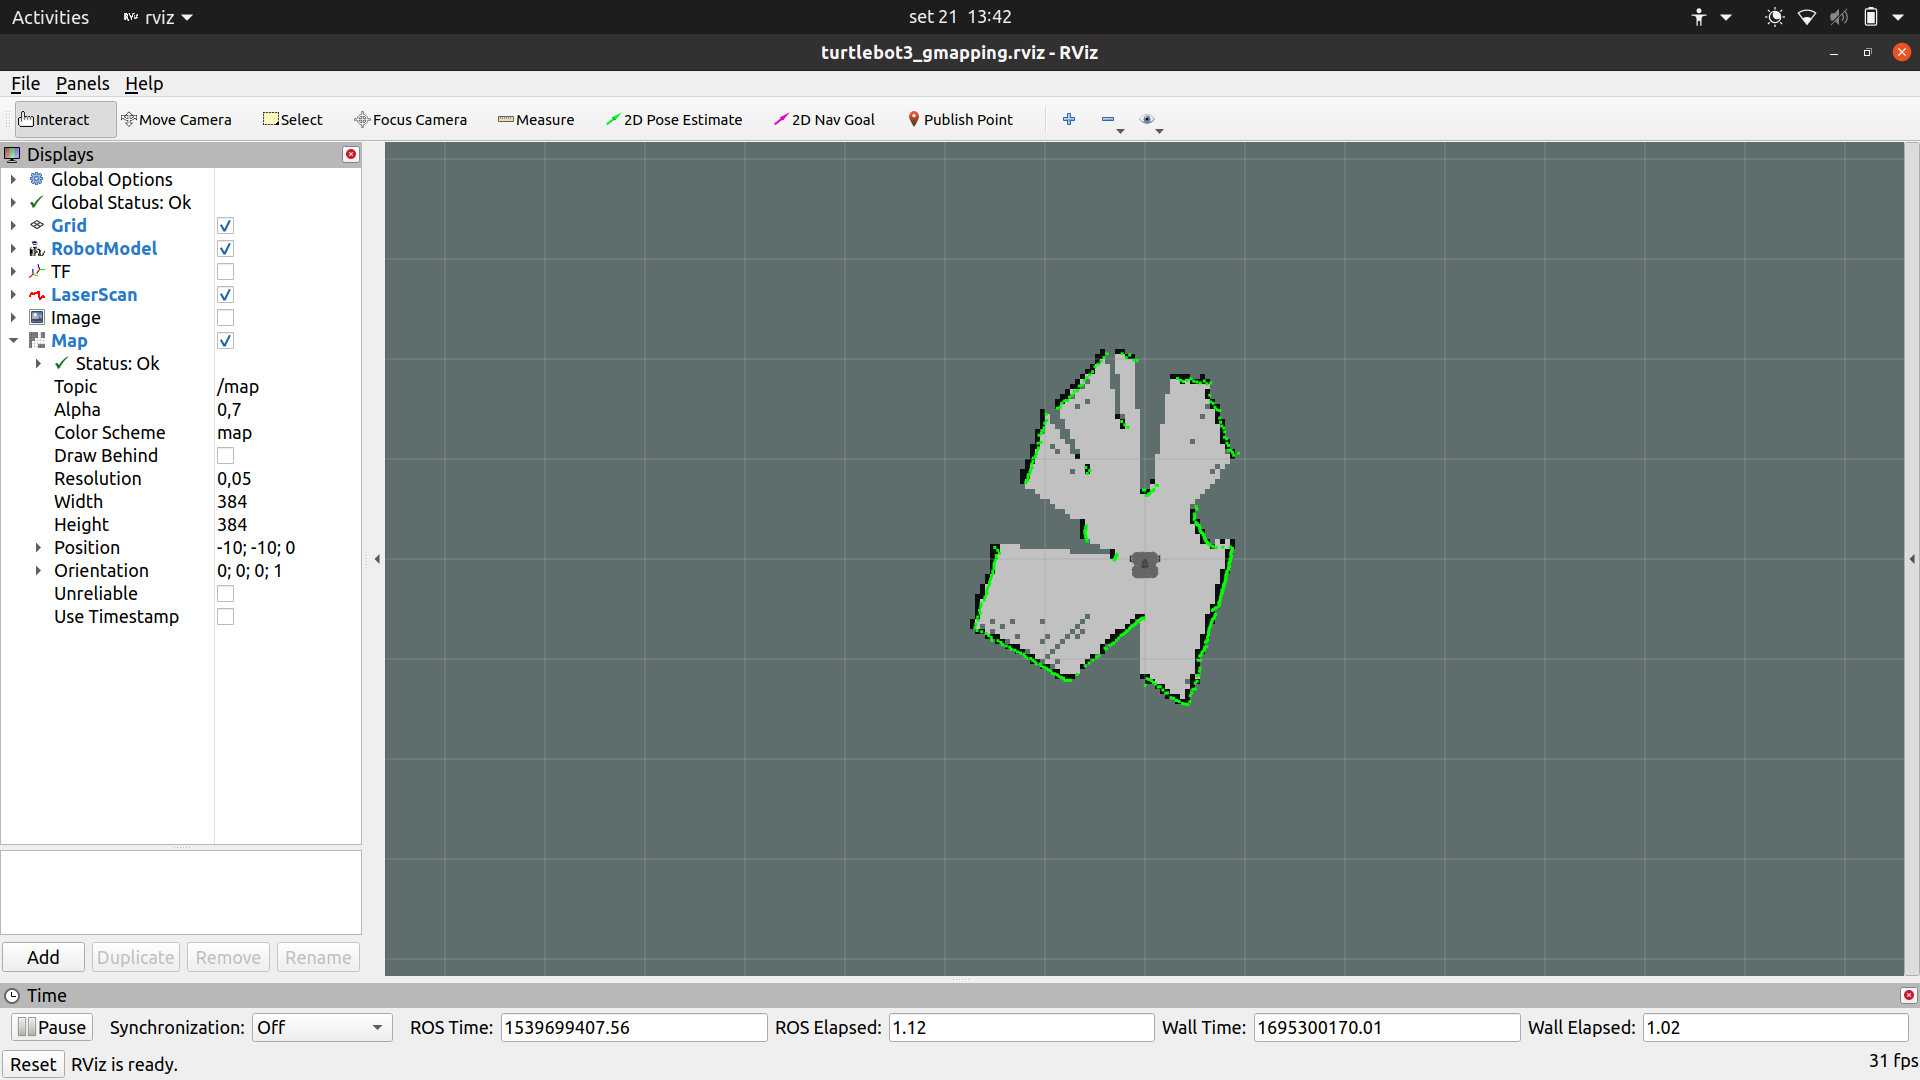
\includegraphics[width=1.0\textwidth]{./Images/dataset_gmapping_initial_map}
\caption{Dataset provided map (still mapping)}
\label{fig:flowchart}
\end{figure}


\begin{figure}[h]
\centering
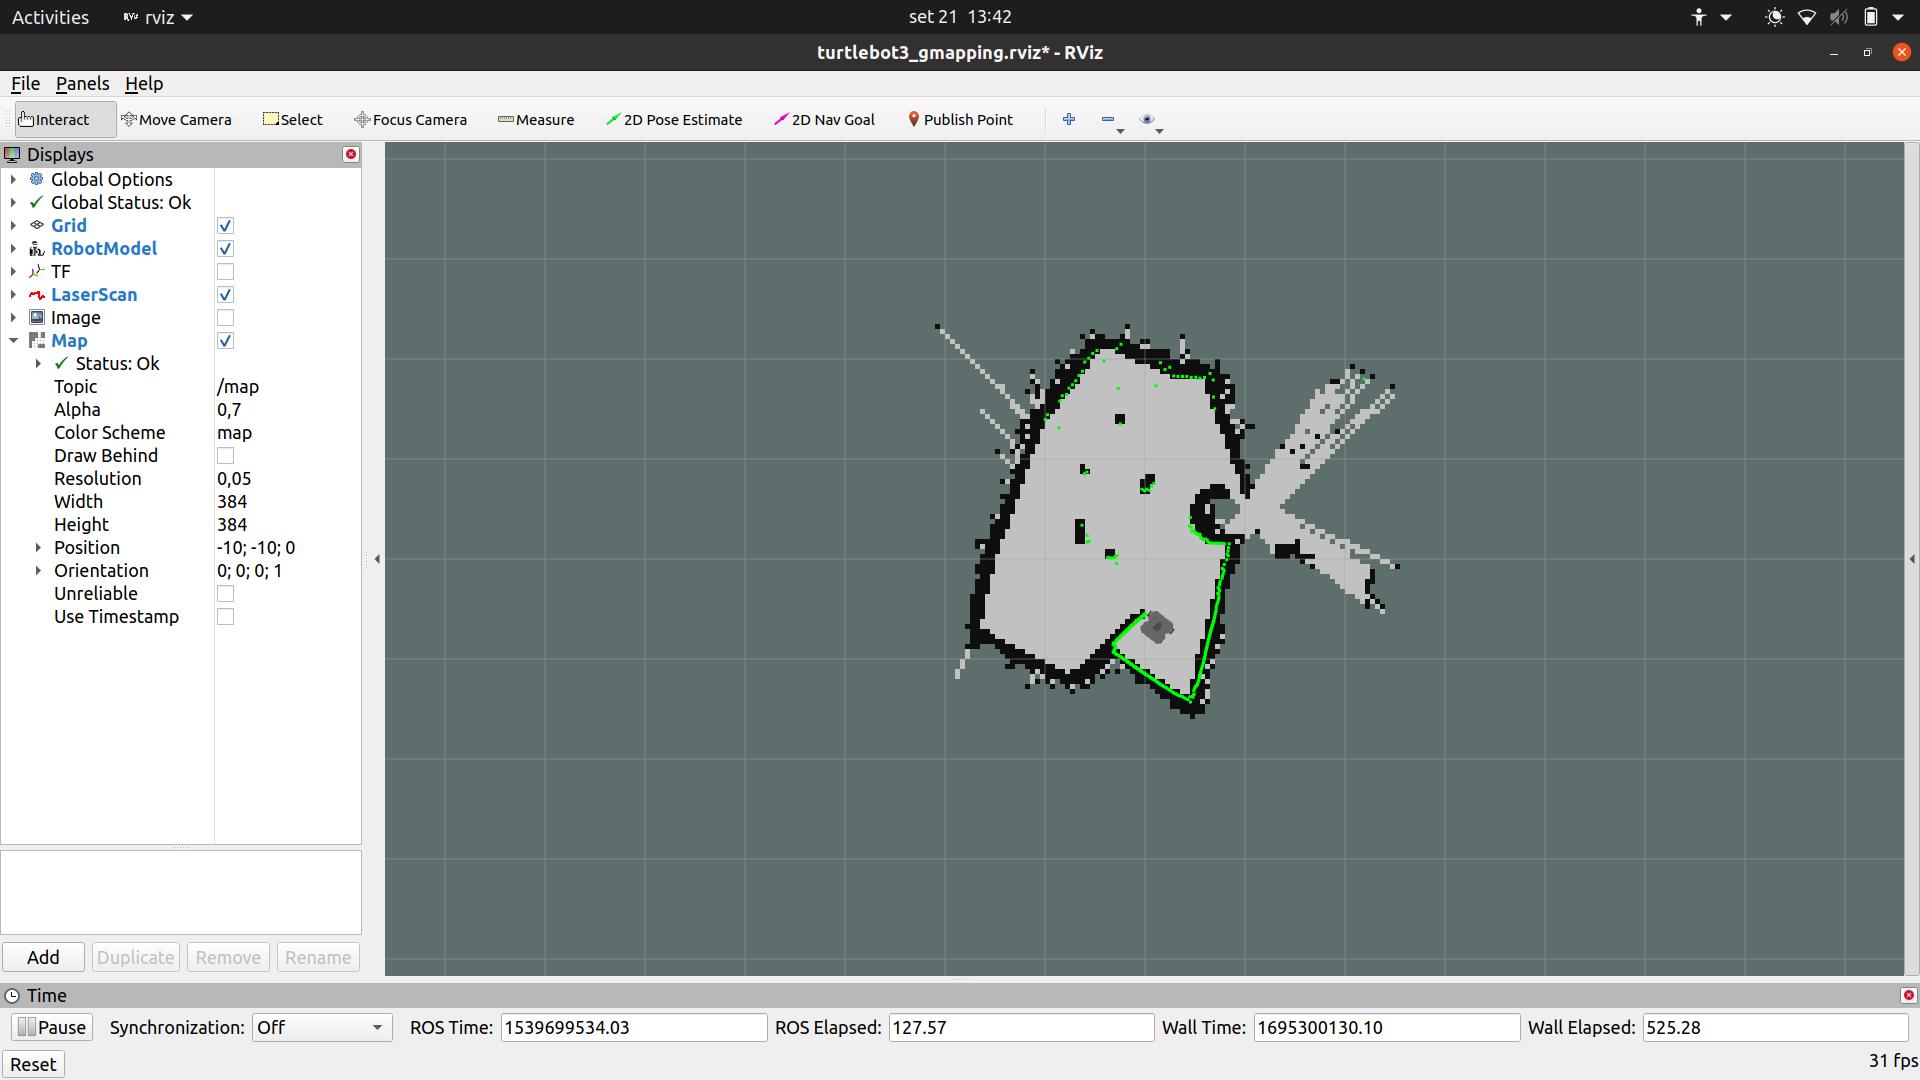
\includegraphics[width=1.0\textwidth]{./Images/dataset_gmapping_final_map}
\caption{Dataset provided map (fully mapped)}
\label{fig:flowchart}
\end{figure}

<Compare gmapping position results with ground thruth>

The same principle was then applied to map the room where we had previously recorded a rosbag. 
The results originated can be visualised in the figure bellow.

\begin{figure}[h]
\centering
\vspace{3pt}
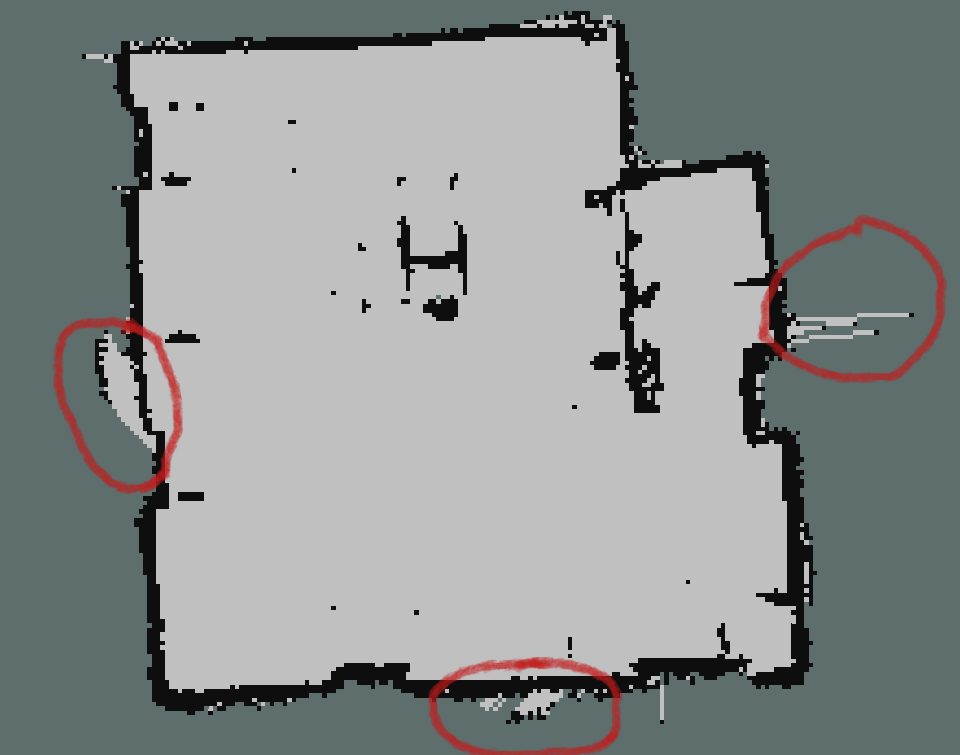
\includegraphics[scale=0.4]{./Images/lsdc4Map}
\caption{LSDC4 room map}
\label{fig:flowchart}
\end{figure}

It is possible to see some noise associated with the image. This can occur due to extent reasons such as: gmapping parameters not being well calibrated; reflections, dynamic objects or other external disturbances; sensor noise and more. The noise is represented in the figure through red circles.
% If Printing on DOUBLE SIDED pages, the second page should be white.
% Otherwise, comment the following command:
\cleardoublepage
%
%Chapter 3
% #############################################################################
% This is Chapter 3
% !TEX root = ../main.tex
% #############################################################################
% Change the Name of the Chapter i the following line
\fancychapter{Localization}
\cleardoublepage
% The following line allows to ref this chapter
\label{chap:architecture}

This chapter explores in detail the comparison between different packages to solve the localization problem. We test three packages, each one using a different approach.
To evaluate the accuracy of each package, we used a provided python script, which computes the difference between the ground truth robot position and the estimated one. This script was adapted to compute the average position error.
% #############################################################################
\section{Ground Truth}

The ground truth is an important piece of data that will let us compare our position estimates with the real robot position in the future. Looking at the github repository where we got the dataset from, it is said the following: `The ground-truth data is provided in the /tf topic, as a transform \(mocap \rightarrow \mathrm{mocap\_laser\_link}\)`.

In order to be able to view the evolution of the ground truth on the map, a script was created. This script, listens to the transformations \(mocap \rightarrow \mathrm{mocap\_laser\_link}\) being published on the /tf topic, retrieves its translation and rotation from the mocap frame and accumulates them on a list. Due to that, it creates a list with all the robot previous positions. It then publishes this list of points on a new topic. Having done so, we can now easily run rviz and add a path that listens to the topic where the accumulated positions are being published. The result of the previous actions can be visualised in the figure ...., where the thin green line represents the real robot path.

\begin{figure}[h]
\centering
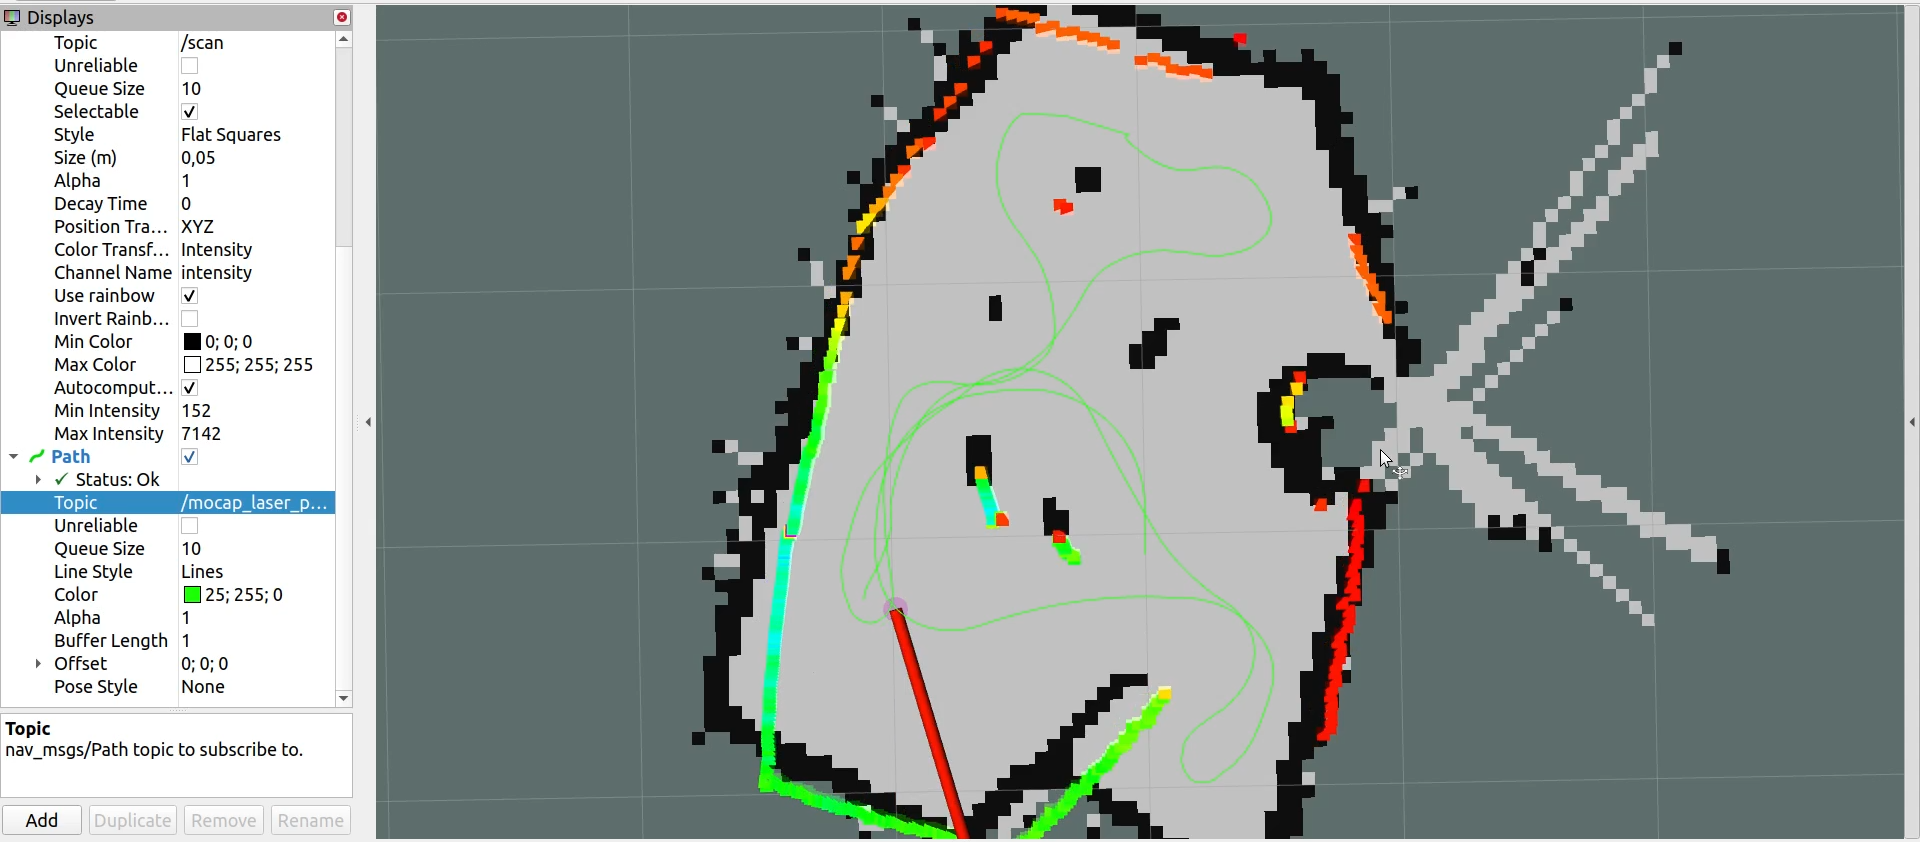
\includegraphics[scale=0.2]{./Images/mocapRviz}
\caption{Robot ground truth path}
\label{fig:flowchart}
\end{figure}

\section{Robot Localization Package}

In this section we will walk you through our progress using the robot localization package, in conjunction with the Extended Karmen Filter algorithm. 

Our first interactions with the ekf algorithm did not go too well. There was a consistent problem of having the robot estimate position outside the map, which can be observed in the figure ....

\begin{figure}[h]
\centering
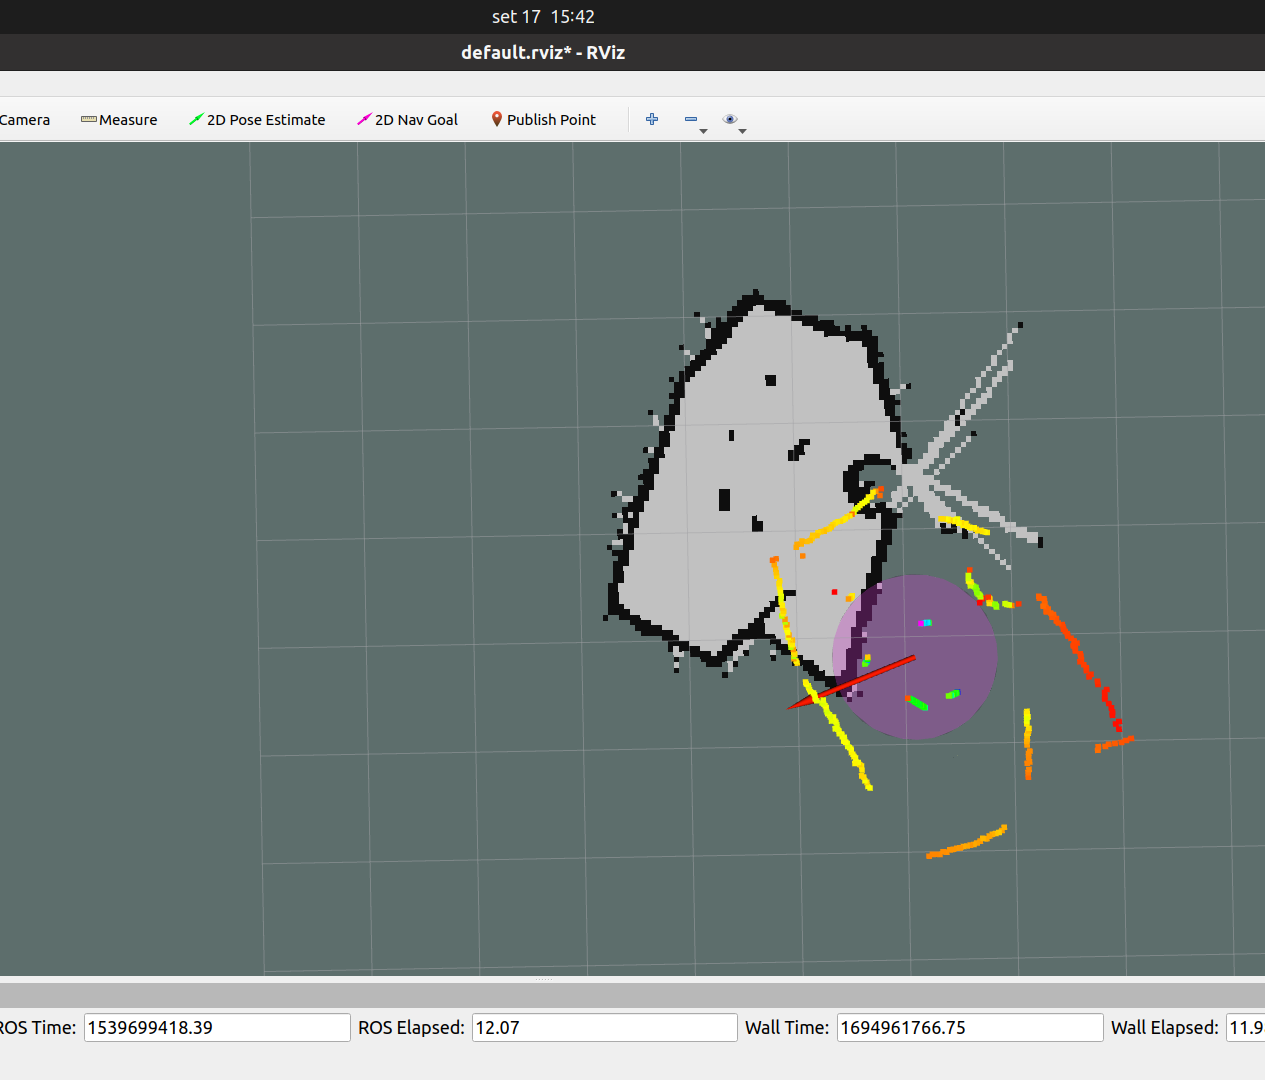
\includegraphics[scale=0.4]{./Images/ekfOutsideMap}
\caption{Using ekf algorithm on the dataset provided map}
\label{fig:flowchart}
\end{figure}

The solution, at first, to this problem was found in the parameters of the robot localization package. There is one particular parameter called "publish\_tf" which when set to false, solved the problem of the laser being readings being outside the map. It also made the error between the robot true position (ground truth) and the robot estimate position, represented by the "base\_scan" frame, smaller than when using the parameter set to true. 

\begin{figure}[h]
\centering
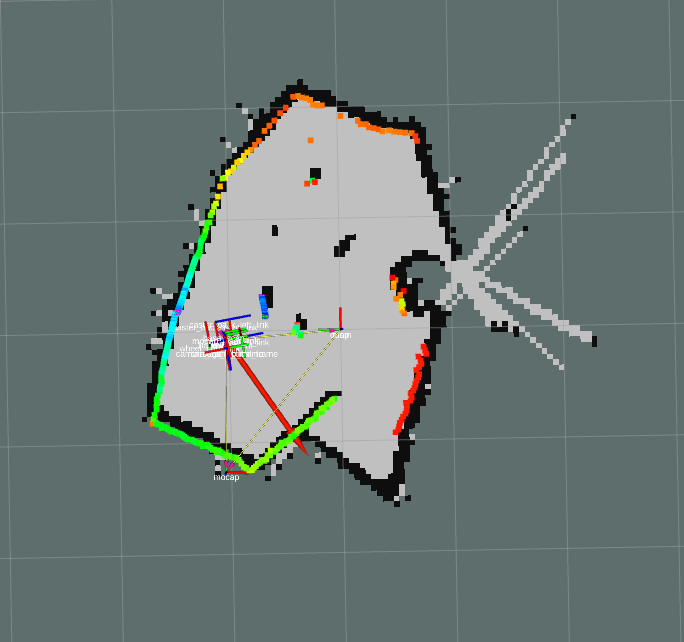
\includegraphics[scale=0.5]{./Images/tfPublishFalse}
\caption{Using the "publish\_tf" parameter set to false}
\label{fig:flowchart}
\end{figure}

Unfortunately, we later found that this could not be the solution to our problem. If we observe the list of topics being published, two of them are relevant to this problem: "/odom" and "/odometry/filtered". They both represent odometry values but their difference is that, while the first one publishes odometry raw data comming from the robot wheel's enconders, the other is the result of using the ekf algorithm with the fused data from the odometry and the imu. In other words, the "/odometry/filtered" topic publishes the position estimated by applying the ekf algorithm, which is what we truly want to test. Returning to the previous solution found, when we set the "publish\_tf" to false, the "base\_scan" frame will represent the raw data from /odom and not the estimated position from /odometry/filtered. Since that, we can not use this solution and must keep the "publish\_tf" parameter set to true.

We will know talk about the final config that we chose for the robot localization package. The parameters that we found more useful were:

\begin{itemize}
    \item Frequency: Increasing the frequency helped reducing the error. This is due to the fact that, since we are making estimates in smaller time intervals, the estimation error will be smaller because the robot traveled less space between estimates and so, it is less uncertain about his current position. Sadly, this technique has some drawbacks. When using greater frequency values some of the message can be lost, making so that when the script to calculate the error was run, it would give different results from run to run. For this reason and after some tests, the value 30 was chosen.
    \item Two D Mode: Since we are operating in an almost totally planar room, for simplicity we set this parameter to true.
    \item Frame: The frame parameters where set up in conformity with the official ros robot localization documentation.
    \item Sensor Config: 
        \begin{itemize}
            \item Odom: 
            \item Imu:
        \end{itemize}
    \item Process Noise Covariance:
    \item Publish Tf: As mentioned before this parameter was set to true.
\end{itemize}

\section{Results On Positioning By Different Algorithms} 

\begin{table}[htb]
\centering
\normalsize
{\footnotesize
    \caption{Position Error Results}
    \label{tab:streamingtech}
    \begin{tabular}{ | c | c | c | c |}
    \hline
    & Gmapping & EKF & AMCL\\
    \hline \hline

    Error (mm) & 37.04 & 64.11 & 43.54 \\
    %\textbf{Protocol} & & & \\ 
    \hline
    
    \end{tabular}
    }
\end{table} 

\section{Changed Parameters} 
\begin{itemize}
    \item imu0\_differential: For each of the sensor messages defined above that contain pose information, users can specify whether the pose variables should be integrated differentially. If a given value is set to true, then for a measurement at time t from the sensor in question, we first subtract the measurement at time t−1, and convert the resulting value to a velocity. This setting is especially useful if your robot has two sources of absolute pose information, e.g., yaw measurements from odometry and an IMU. In that case, if the variances on the input sources are not configured correctly, these measurements may get out of sync with one another and cause oscillations in the filter, but by integrating one or both of them differentially, we avoid this scenario. (EXPLICAR MELHOR ISTO)
\end{itemize}

\section{AMCL}
To estimate/obtain robot localization, it is also possible to use another package: AMCL. This package implements the adaptive (or KLD-sampling) Monte Carlo localization approach (as described by Dieter Fox), which uses a particle filter to track the pose of a robot against a known map. For this experimentation, we also used a recorded rosbag, capture from the IST LAB, using the Turtlebot\_3. The results were observed using the RVIZ programm.

\subsection{Main Principle}
This algorithm, at runtime, will start by spreading the particle number at the initial position (initial robot location estimate). Then, it makes a prediction of the robot location, based on the odometry (maybe IMU too?). Then, it compares the prediction with the laser scan (new mesurements), and updates the particles weights. Next, it resamples the particles, based on the weights, meaning it will discard the particles with lower weights, and will duplicate the particles with higher weights. It repeats the process over and over. 
Overall, with time, the particles will follow a possible robot location.

\subsection{Test Conditions And Expected Results}
For this test, the robot was teleoperated, in the LSD4 LAB, with the map in the image (REFERENCIAR IMAGEM), computed previously. The initial true position is x:0 and y:0. This means that if we already give the correct initial position, the number of particles will meet the true robot position, and the algorithm will quickly converge to the true robot position.
Yet, to test how the number of particles affect this algorithm, we first start to change the initial position to other values, away from the original one. Only after that, we changed the particle number, to try to compensate for the bad initial position.

One important note is that the Ground Thruth is not availbale, and so, the only option to acess how effective the algorithm is progressing, is to observe the estimated path in the RVIZ. (TALVEZ TENTAR ARRANJAR UMA FORMA MELHOR DE PRODUZIR RESULTADOS!)


\begin{figure}[h]
\centering
\vspace{3pt}
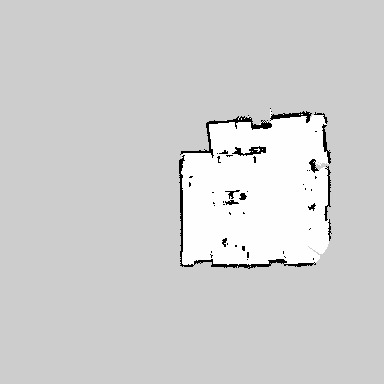
\includegraphics[scale=0.4]{./Images/2023-09-18-10-18-29}
\caption{LSDC4 room map}
\label{fig:flowchart}
\end{figure}


\subsection{Tuning Parameters}
At the moment of writing, the only parameters changed were the MIN and MAX number of particles. We are assuming the number of particles, at runtime, might change between the MIN and MAX set. For instance, if the algorithm is very sure of its estimate, it reduces the particles number. Otherwise, it might increase the particle number. This was not yet confirmed by trustable sources (CONFIRMAR ISTO / TALVEZ NEM SEJA IMPORTANTE).

At first, we started with a conservative number of particles, with particles between 500 and 3000, being the AMCL ROS package default value. We also set the initial algorithm estimate to the true position. The results show that the estimated position seem correct, since the laser readings match the map boundaries \ref{fig:amcl-lab-rosbag-0-0-500-3000}.
\begin{figure}
    \centering
    \includegraphics[width=1\linewidth]{Images/amcl-lab-rosbag-0-0-500-3000.drawio.png}
   \caption{AMCL iteration, with correct initial position (x:0, y:0), and default number of particles ([500-3000])}
    \label{fig:amcl-lab-rosbag-0-0-500-3000}
\end{figure}

Then, we proceed to alter the initial AMCL position (but not the number of particles), a bit to the right. The results show that the AMCL tries to correct the estimated position, a bit to the left \ref{fig:amcl-lab-rosbag--1--1-500-3000}.

\begin{figure}
    \centering
    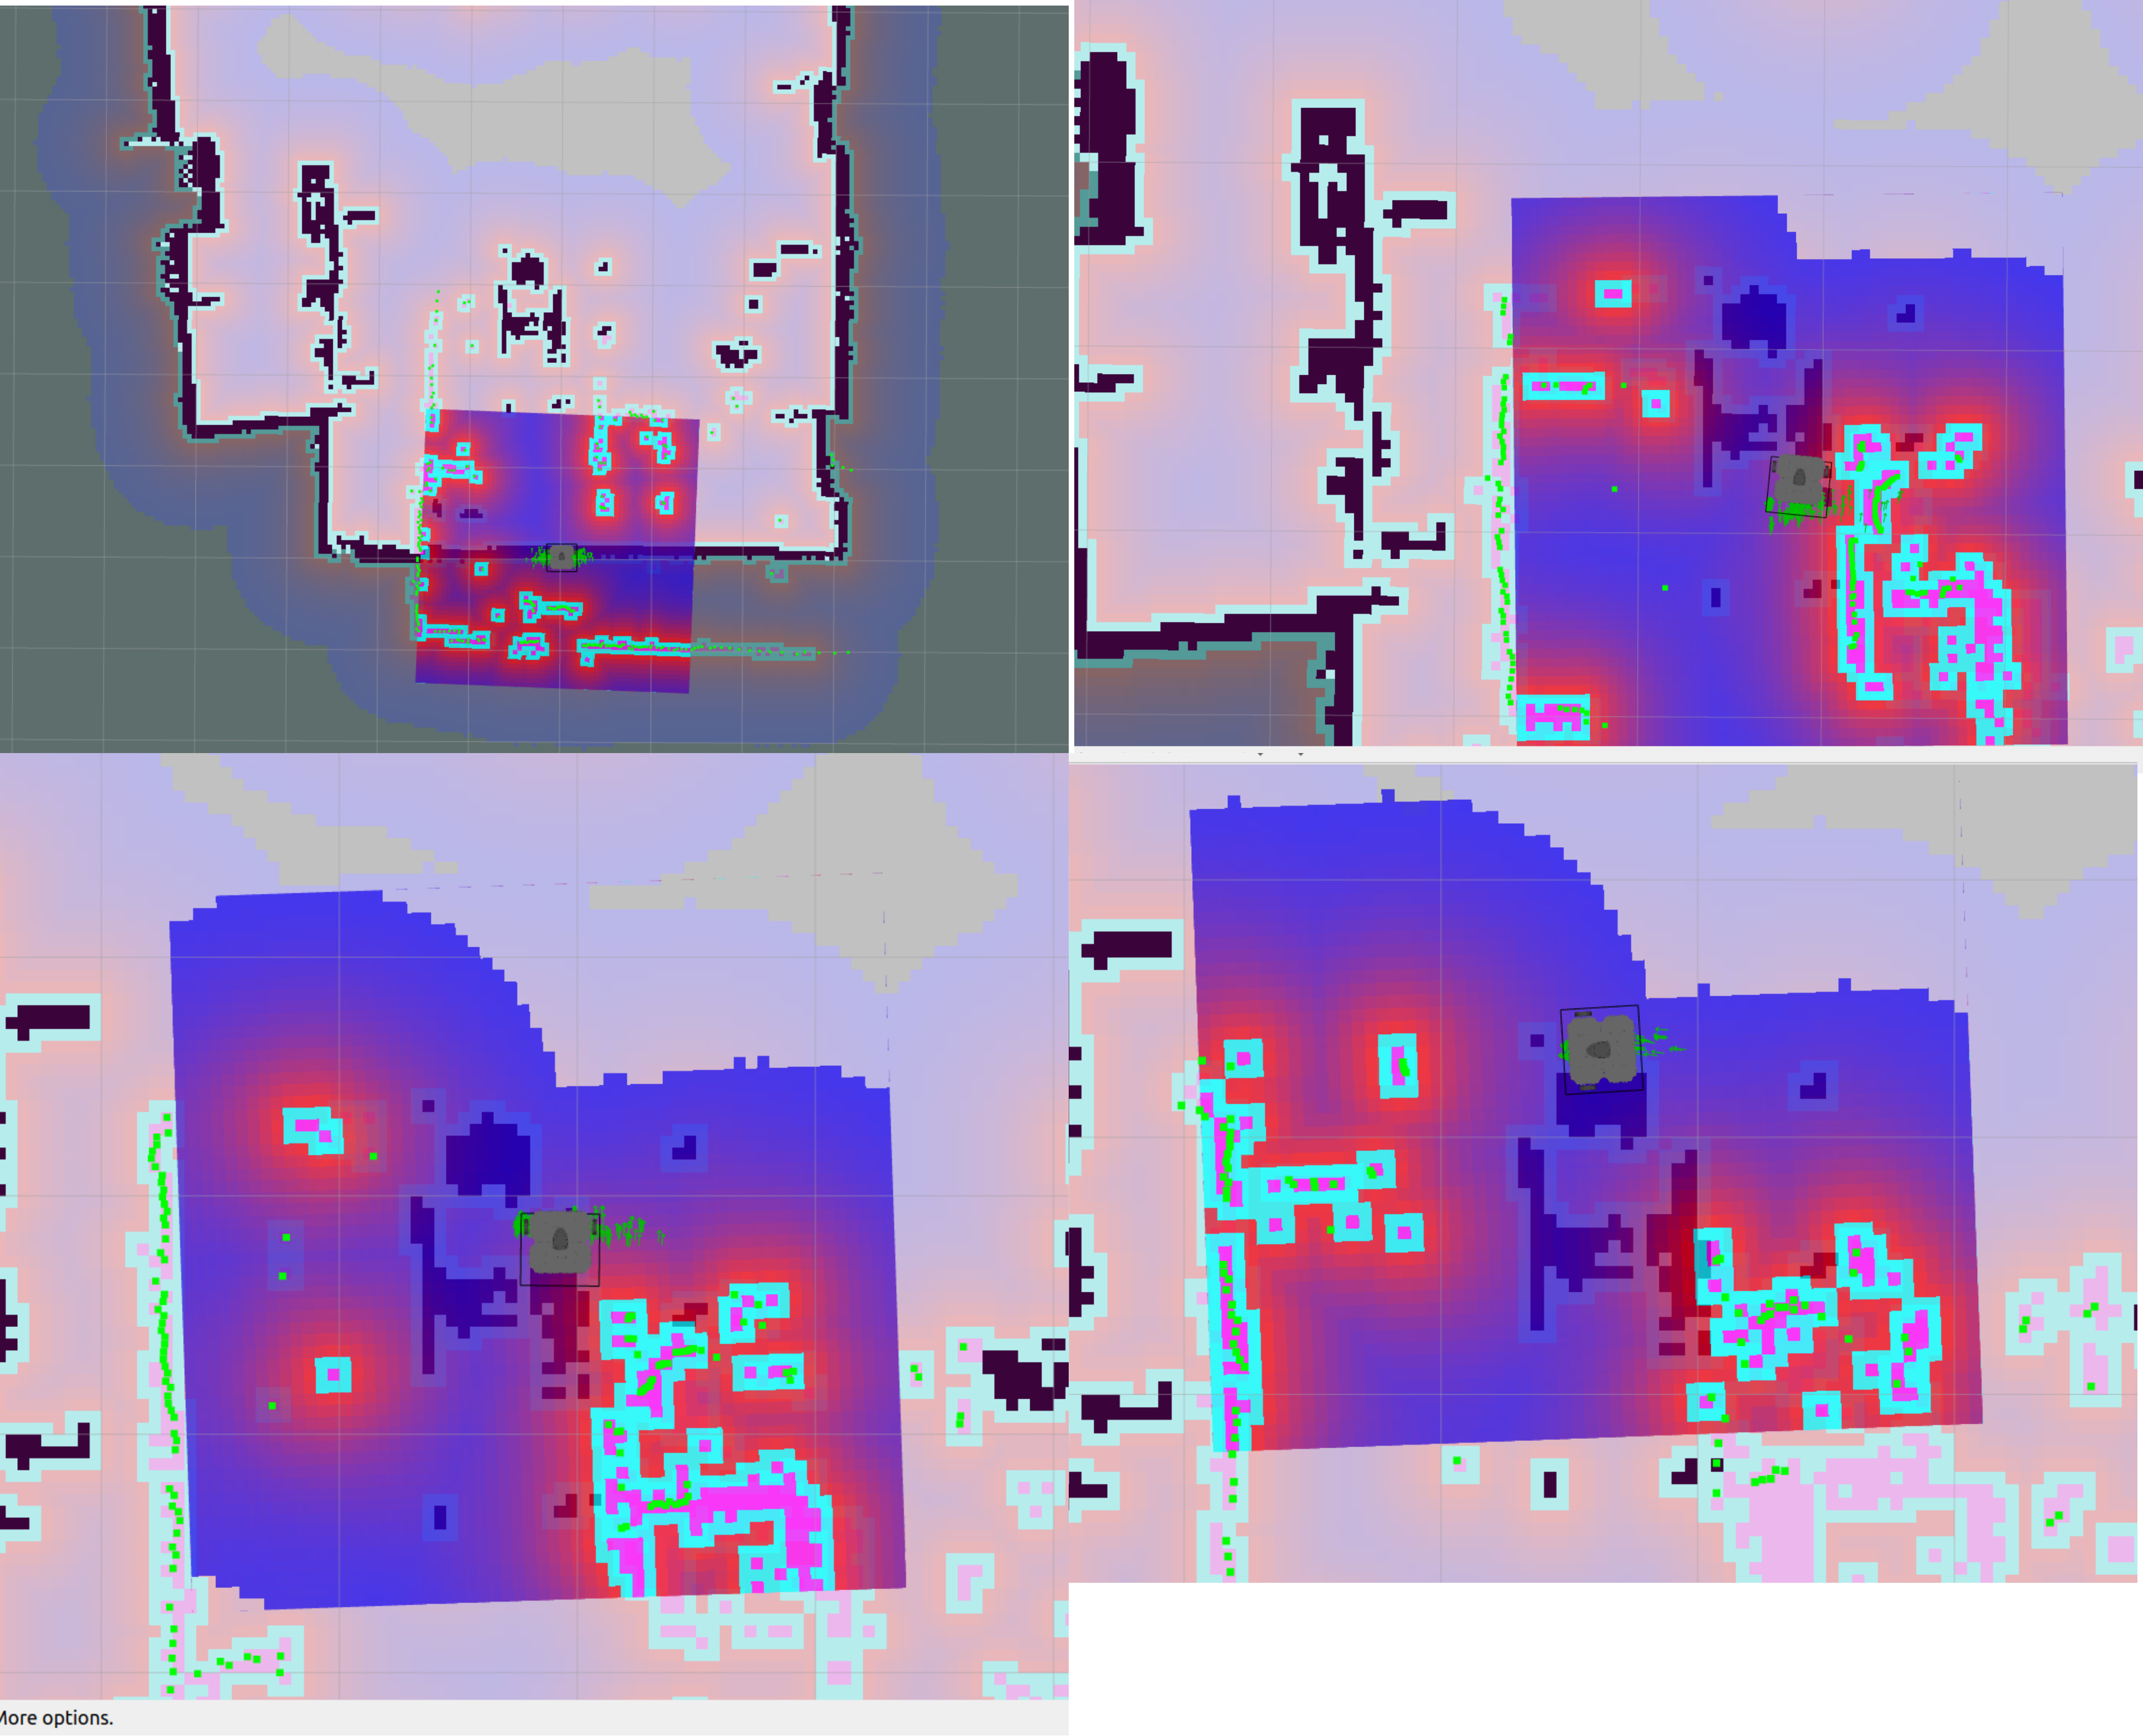
\includegraphics[width=1\linewidth]{AMCL iteration, (x -1, y -1)-([500-3000]).png}
    \caption{AMCL iteration, with wrong initial position (x:-1, y:-1), and default number of particles ([500-3000])}
    \label{fig:amcl-lab-rosbag--1--1-500-3000}
\end{figure}

Yet, this correct is not very noticeable. To allow for a better comparison, the particles were duplicated (from [500-3000] to [1000-6000]). The results show a big increase in the correction shift \ref{fig:amcl-lab-rosbag--1--1-1000-6000 - first iter}.

\begin{figure}
    \centering
    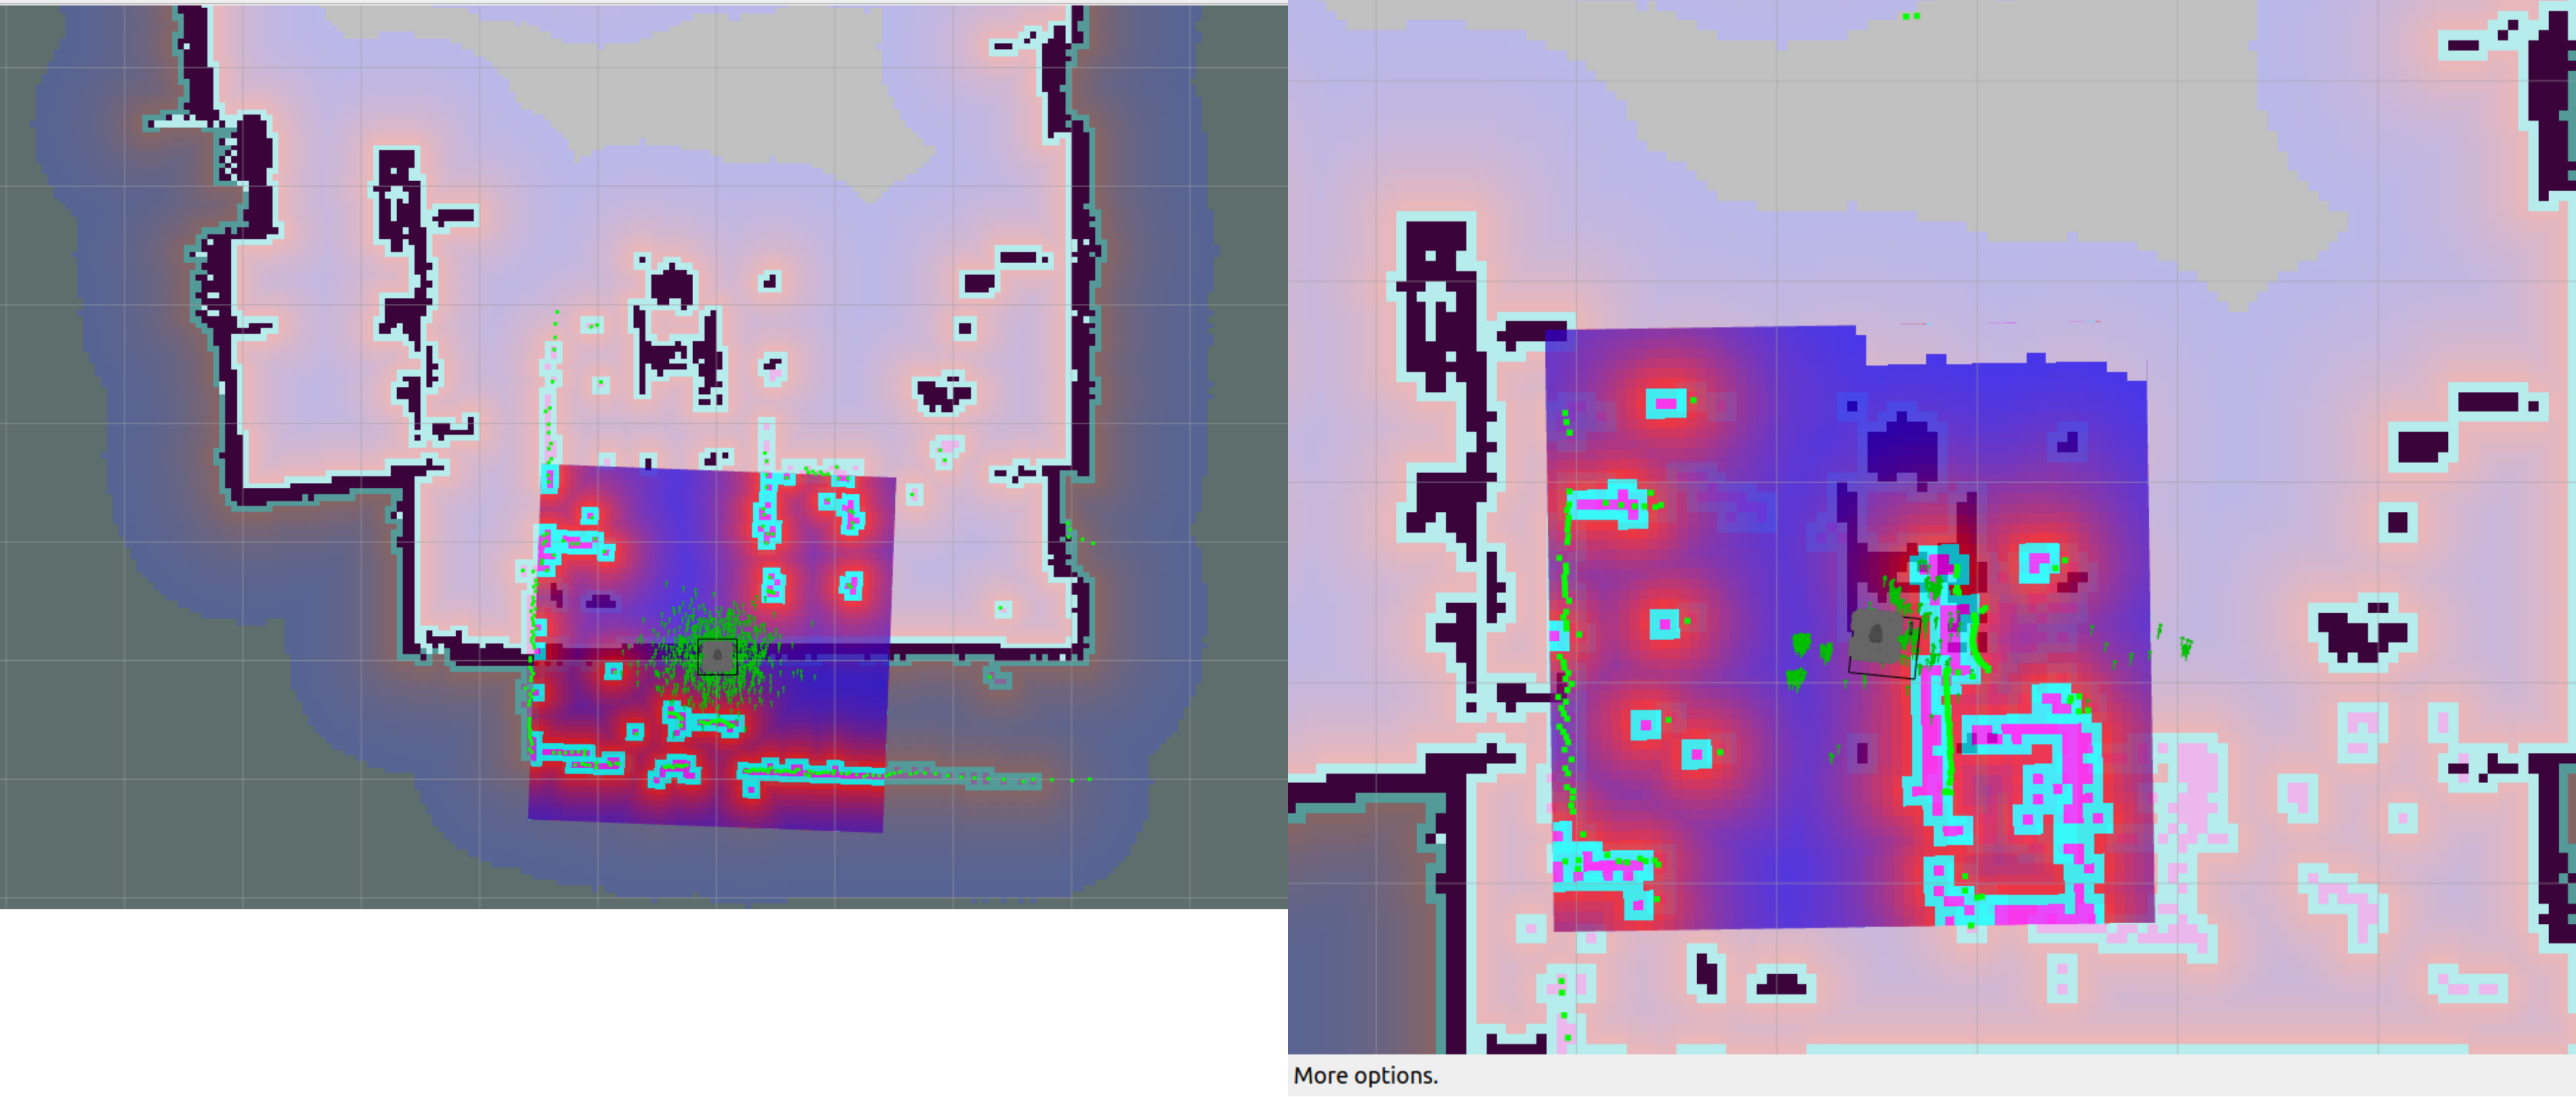
\includegraphics[width=1\linewidth]{AMCL iteration, (x -1, y -1)-([500-3000])(1).png}
    \caption{AMCL iteration, with wrong initial position (x:0, y:0), and default number of particles ([500-3000]) - First Iteration}
    \label{fig:amcl-lab-rosbag--1--1-1000-6000 - first iter}
\end{figure}

This means that the algorithm tends to converge to the correct position much faster when the number of particles is increased. This can be explained duo to the probability of existing particles in the right robot pose being much higher, which will then receive more weights, leading to a faster convergence.

Then, the same test was conducted, exacly with the same parameters as in the last paraghraph. The results continued to show a level of correction shift to the left, but not as accentuated as preveouly \ref{fig:amcl-lab-rosbag--1--1-1000-6000 - second iter}. 
This happens because when the AMCL algorithm starts, the initial destribution of particles is random. In the first iteration, by pure chance, the particle destribution was probably closer to the true robot's pose, leading to a better and faster correction. 

\begin{figure}
    \centering
    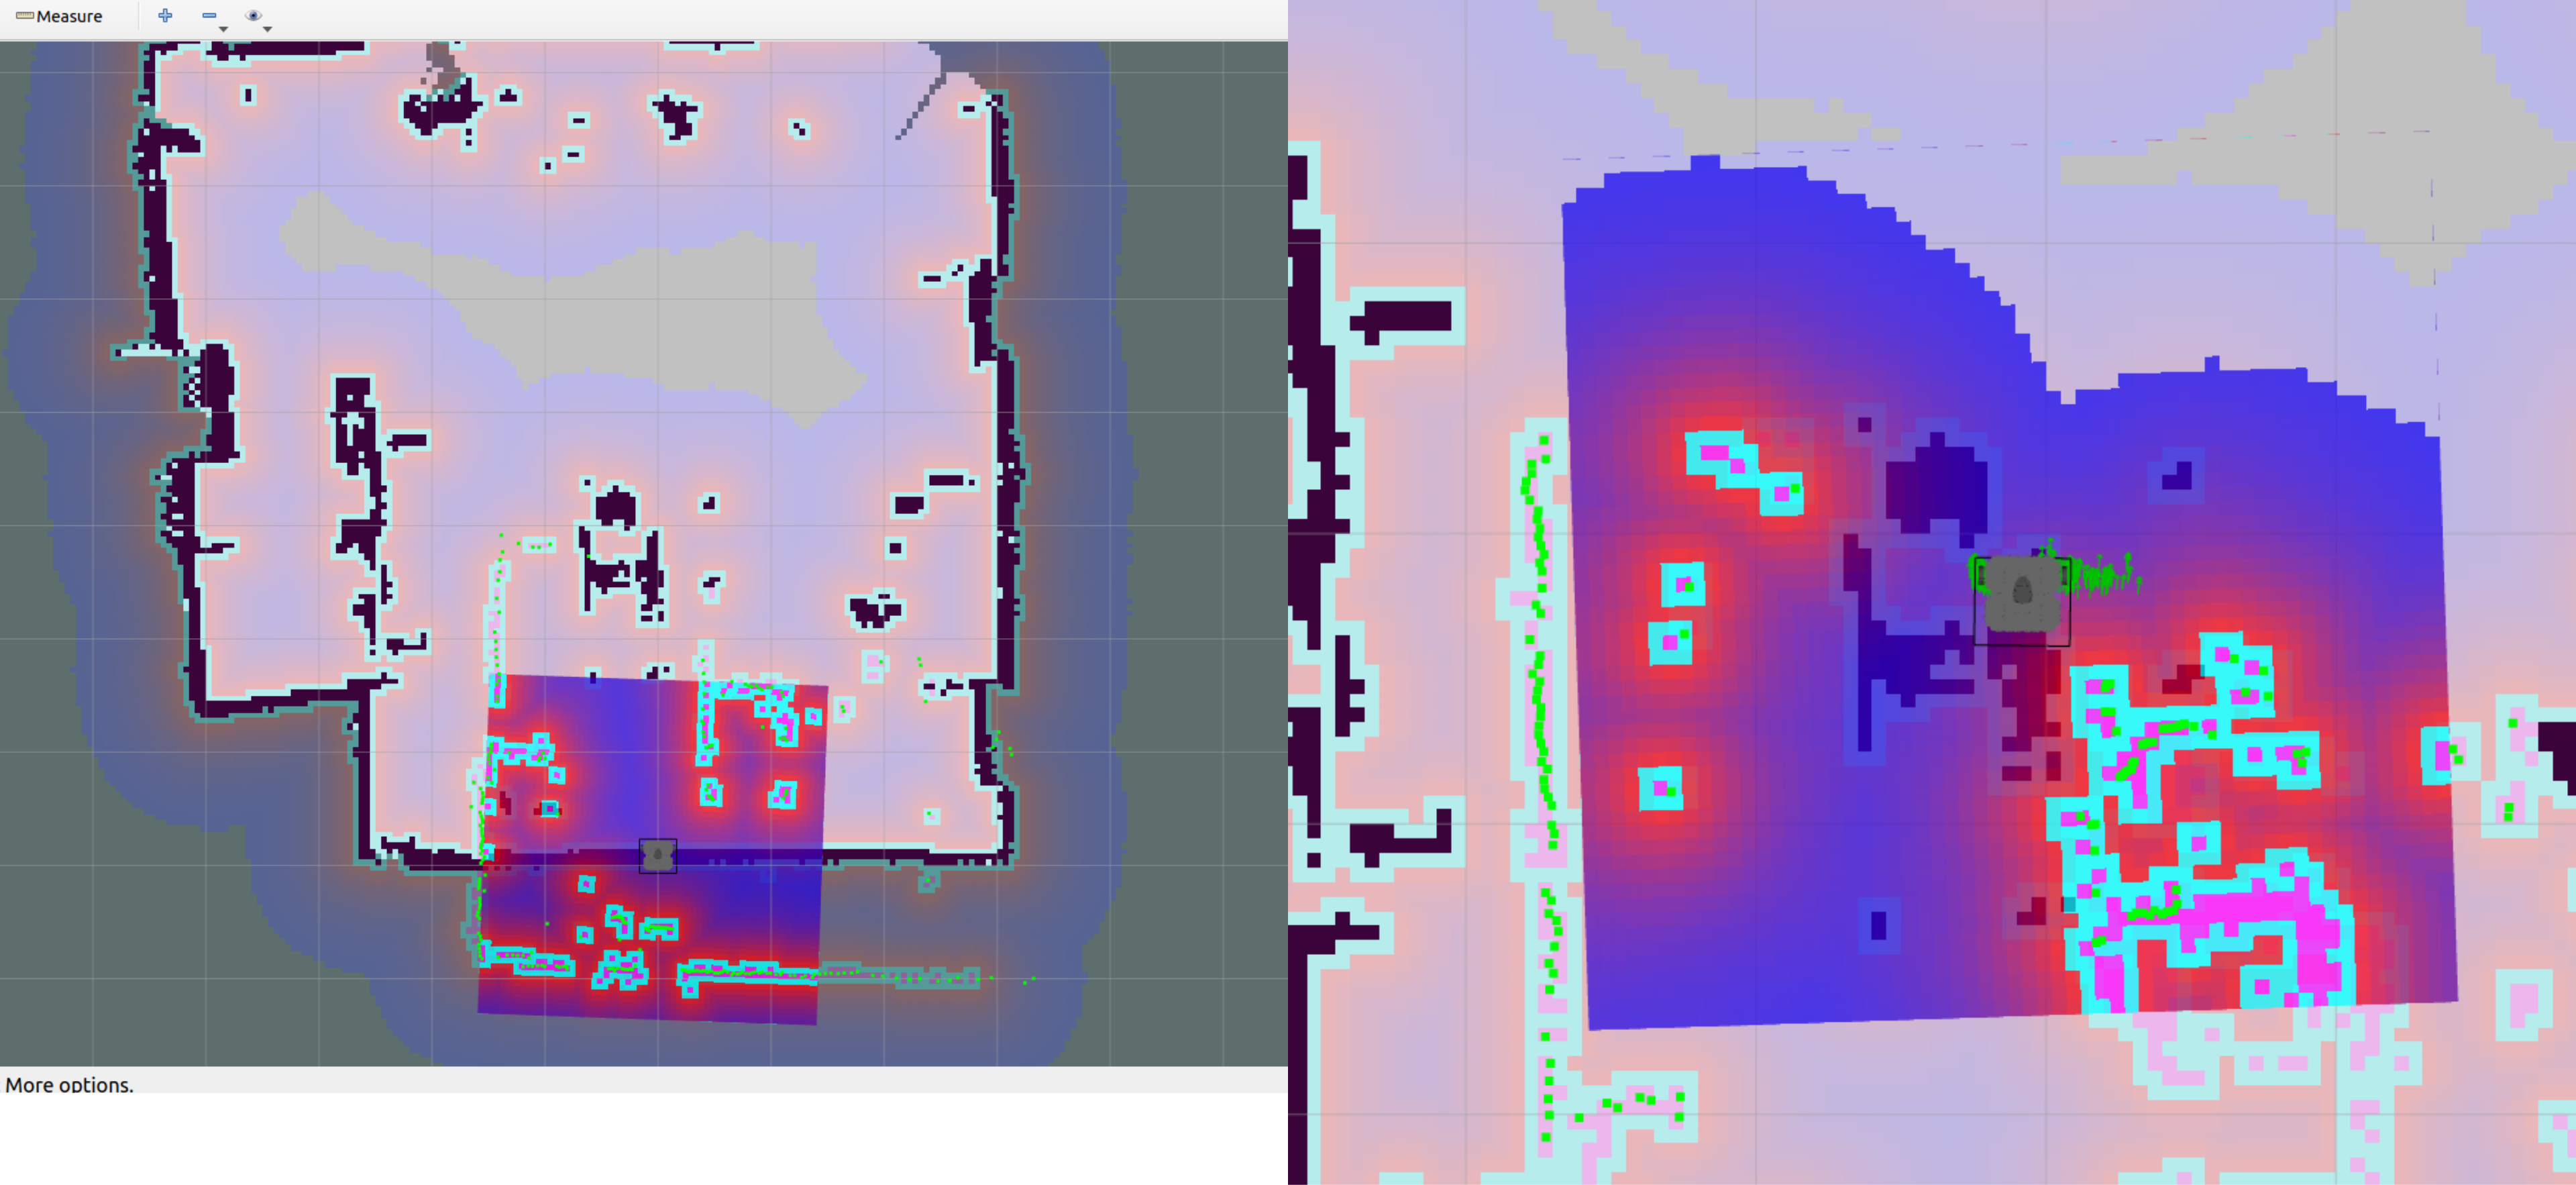
\includegraphics[width=1\linewidth]{amcl-lab-rosbag--1--1-1000-6000.png}
    \caption{AMCL iteration, with wrong initial position (x:0, y:0), and default number of particles ([500-3000]) - Second Iteration}
    \label{fig:amcl-lab-rosbag--1--1-1000-6000 - second iter}
\end{figure}

Finally, and to confirm the effect of the number of particles in the algorithm's performance, this one was lowered to just one particle, \ref{fig:amcl-lab-rosbag--1--1-1-1}. The results showed that no or little correction was made. This can be explained since one particle is not enough to explore the "environment" and thus, the probability of matching the real pose, when the robot receives new sensor measurements, is very low. 

\begin{figure}
    \centering
    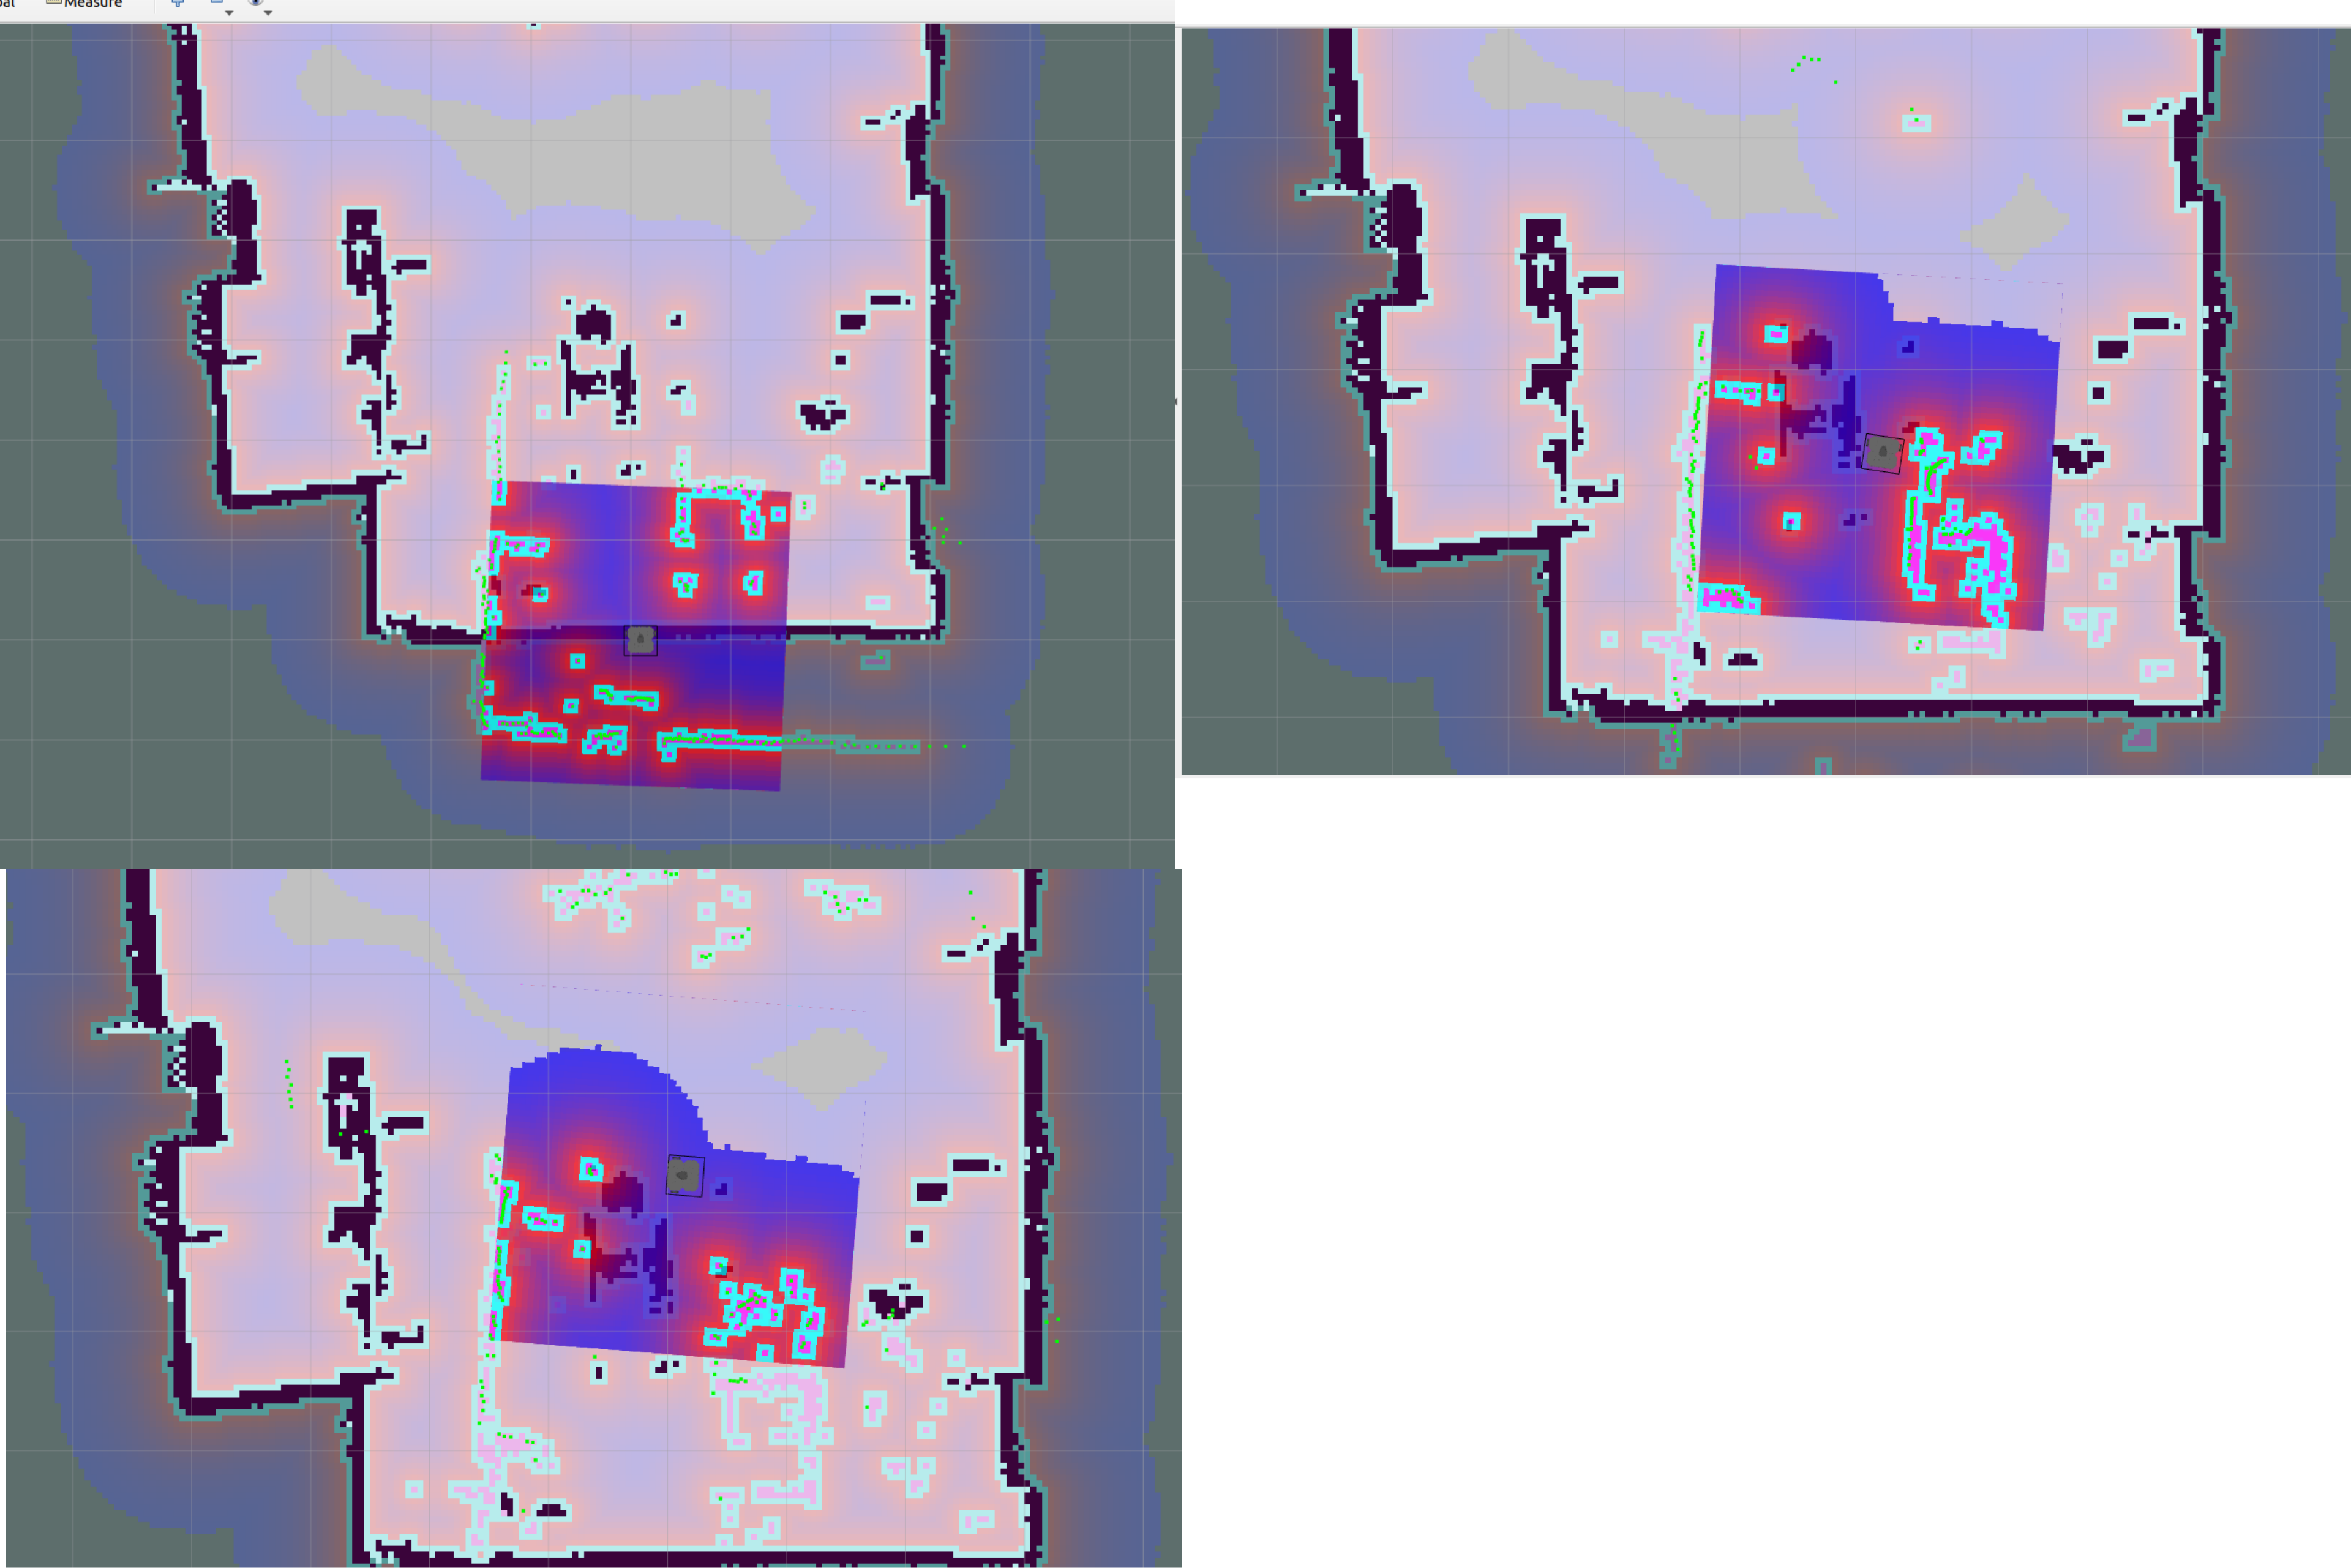
\includegraphics[width=1\linewidth]{amcl-lab-rosbag--1--1-1-1.png}
        \caption{AMCL iteration, with wrong initial position (x:0, y:0), and default number of particles ([1-1])}
    \label{fig:amcl-lab-rosbag--1--1-1-1}
\end{figure}

Now, lets see something interesting... Instead of placing the AMCL initial position shifted to the right, the initial position will be shifted to the left: (x:1, y:1). The number of particles stays the same as the default value: [500-3000]. The results \ref{fig:amcl-lab-rosbag-1-1-500-3000} show that, instead of shifting the robot's position to the right, in order to correct the initial right shifted position, the AMCL is actually shifting the robot to the left. Even when the number of particles is actually raised to 30000, the same thing happens most of the time \ref{fig:amcl-lab-rosbag-1-1-30000-30000}. {AINDA NAO SEI EXPLICAR ISTO}. If the number of particles is raised, the AMCL will use more data from new sensorial measurement to correct the estimated pose. If the corrections are being made in the oposite direction, this means that the particles are matching the wrong sensor mesurements. {SERA ESTA A CAUSA???}

Yet, this doesn't happen if the number of particles is again set to 1 (minimum value) \ref{fig:amcl-lab-rosbag-1-1-1-1}. The reason is because, since there is only one particle, the algorithm is going to use mostly the estimated pose, from the motion and not the measurement model. This explains why there is not left shift, as in the previous example.

\begin{figure}
    \centering
    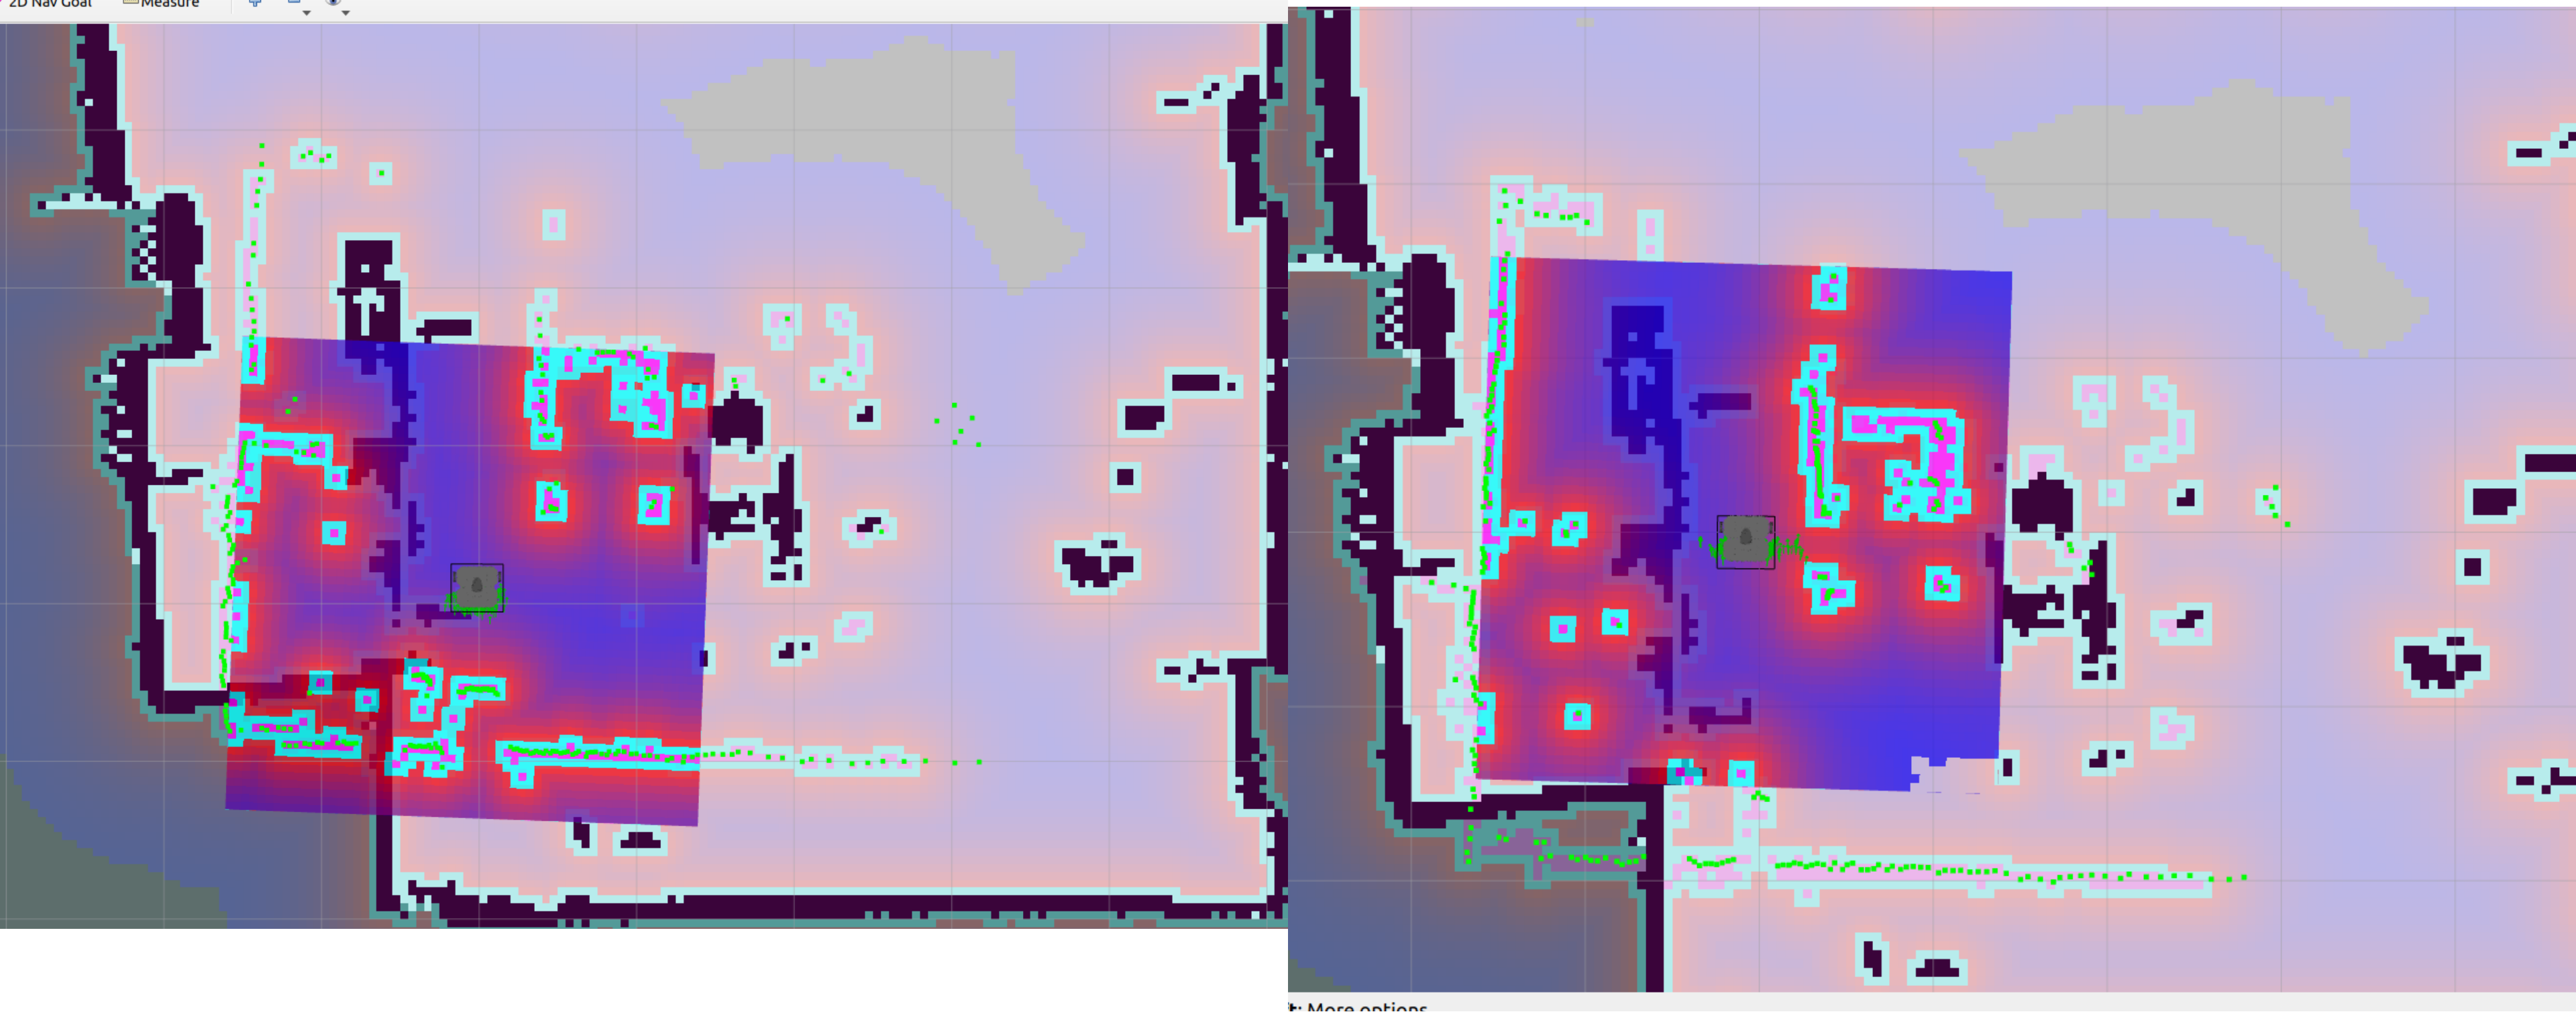
\includegraphics[width=1\linewidth]{amcl-lab-rosbag-1-1-500-3000.png}
    \caption{AMCL iteration, with wrong initial position (x:1, y:1), and default number of particles ([500-3000])}
    \label{fig:amcl-lab-rosbag-1-1-500-3000}
\end{figure}

\begin{figure}
    \centering
    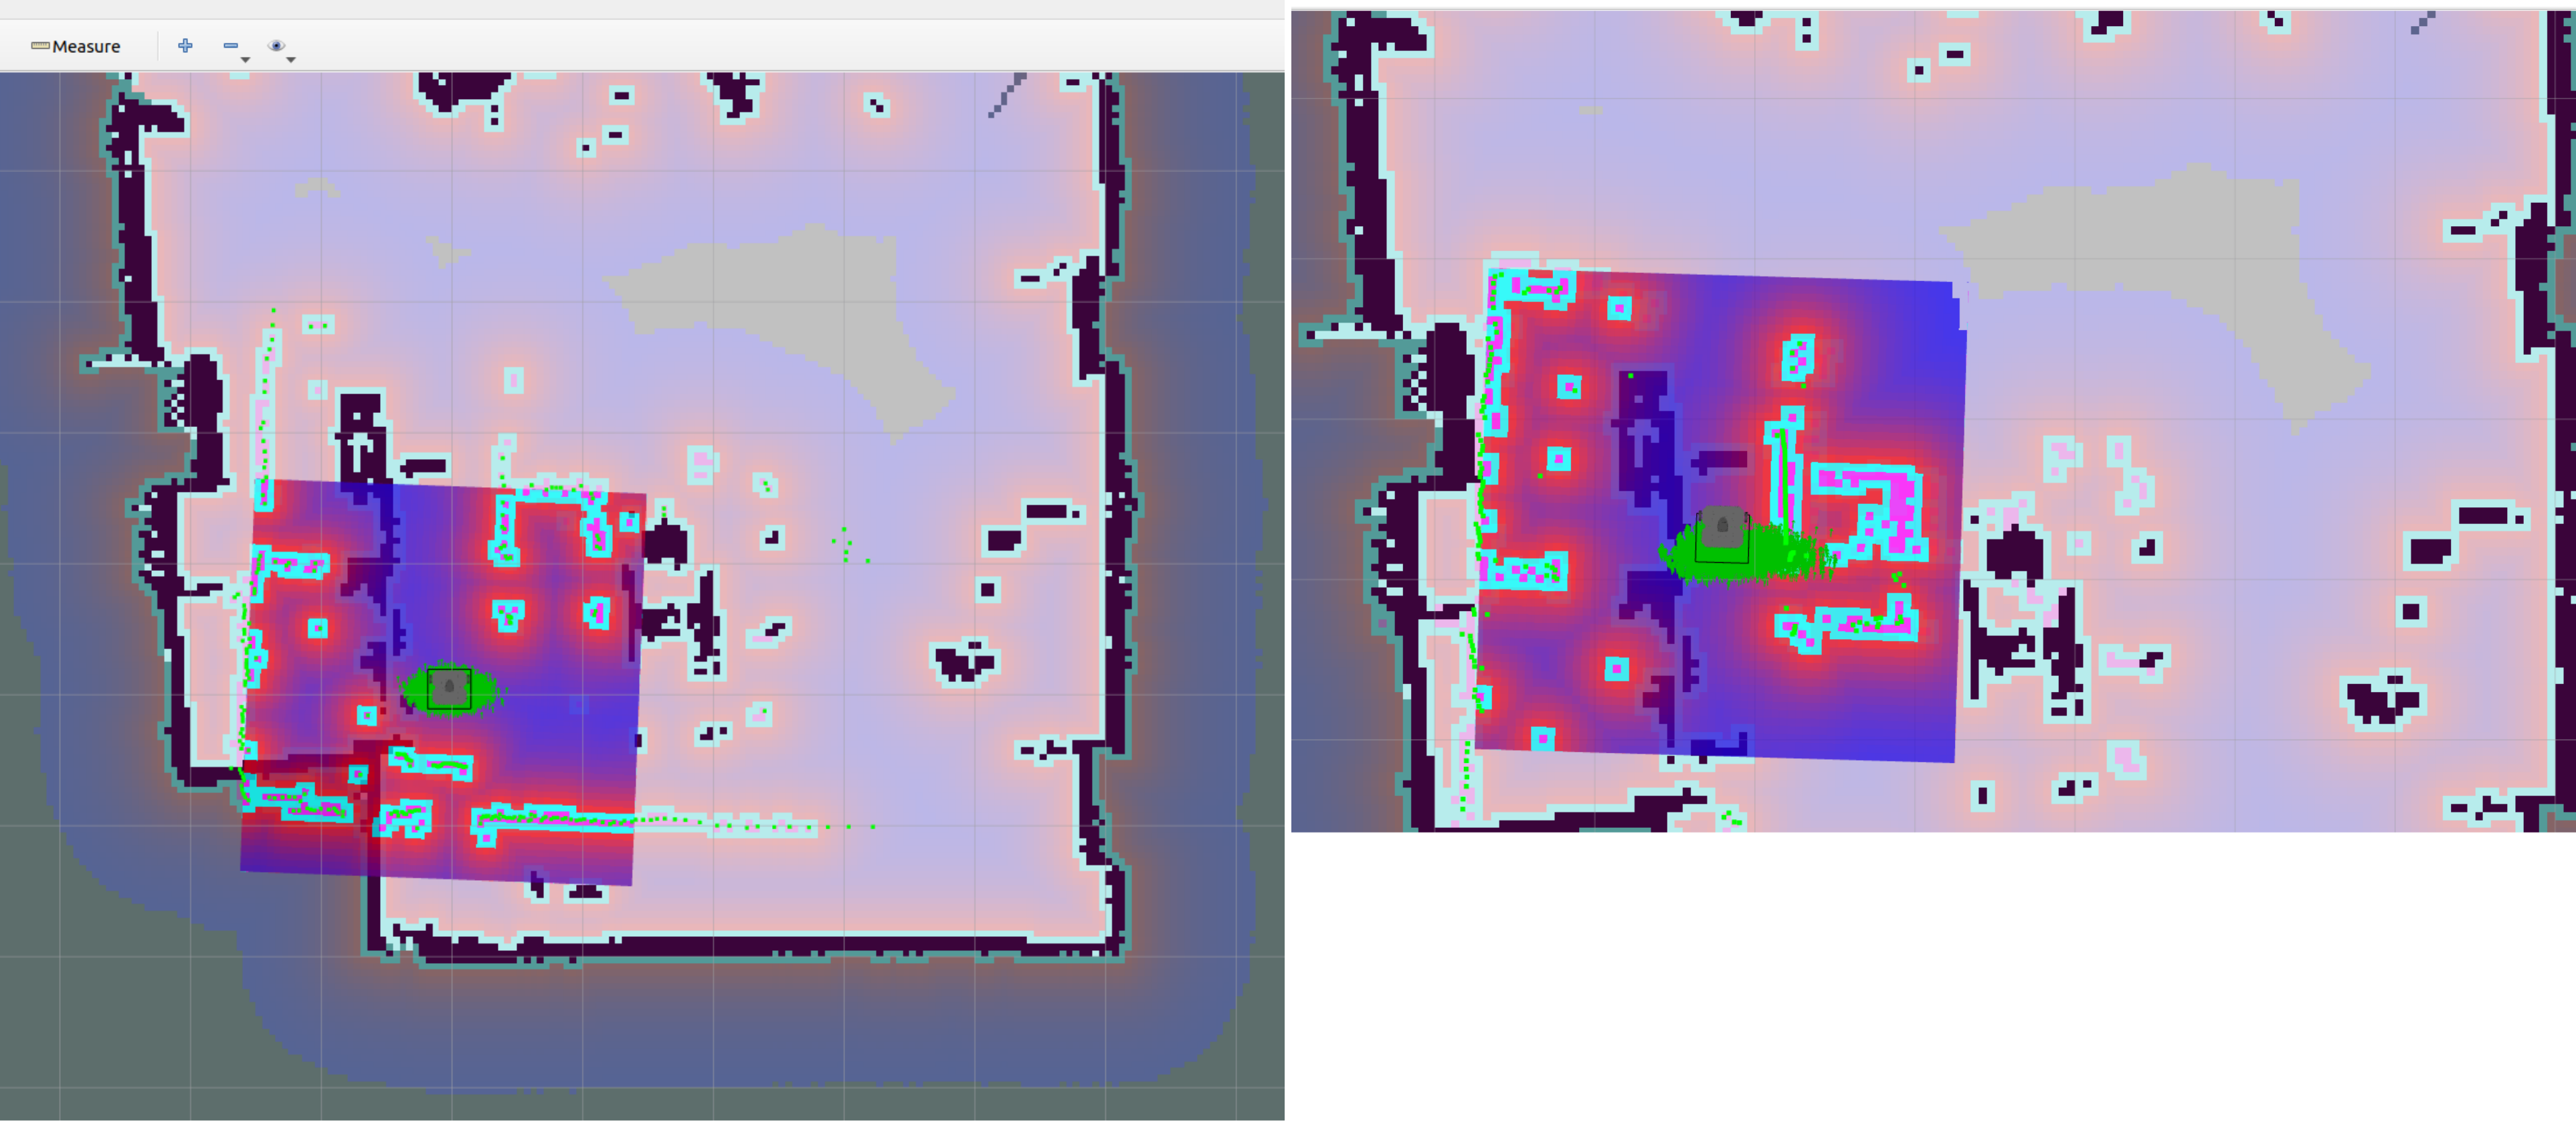
\includegraphics[width=1\linewidth]{amcl-lab-rosbag-1-1-30000-30000.png}
    \caption{AMCL iteration, with wrong initial position (x:1, y:1), and default number of particles ([30000-30000])}
    \label{fig:amcl-lab-rosbag-1-1-30000-30000}
\end{figure}

\begin{figure}
    \centering
    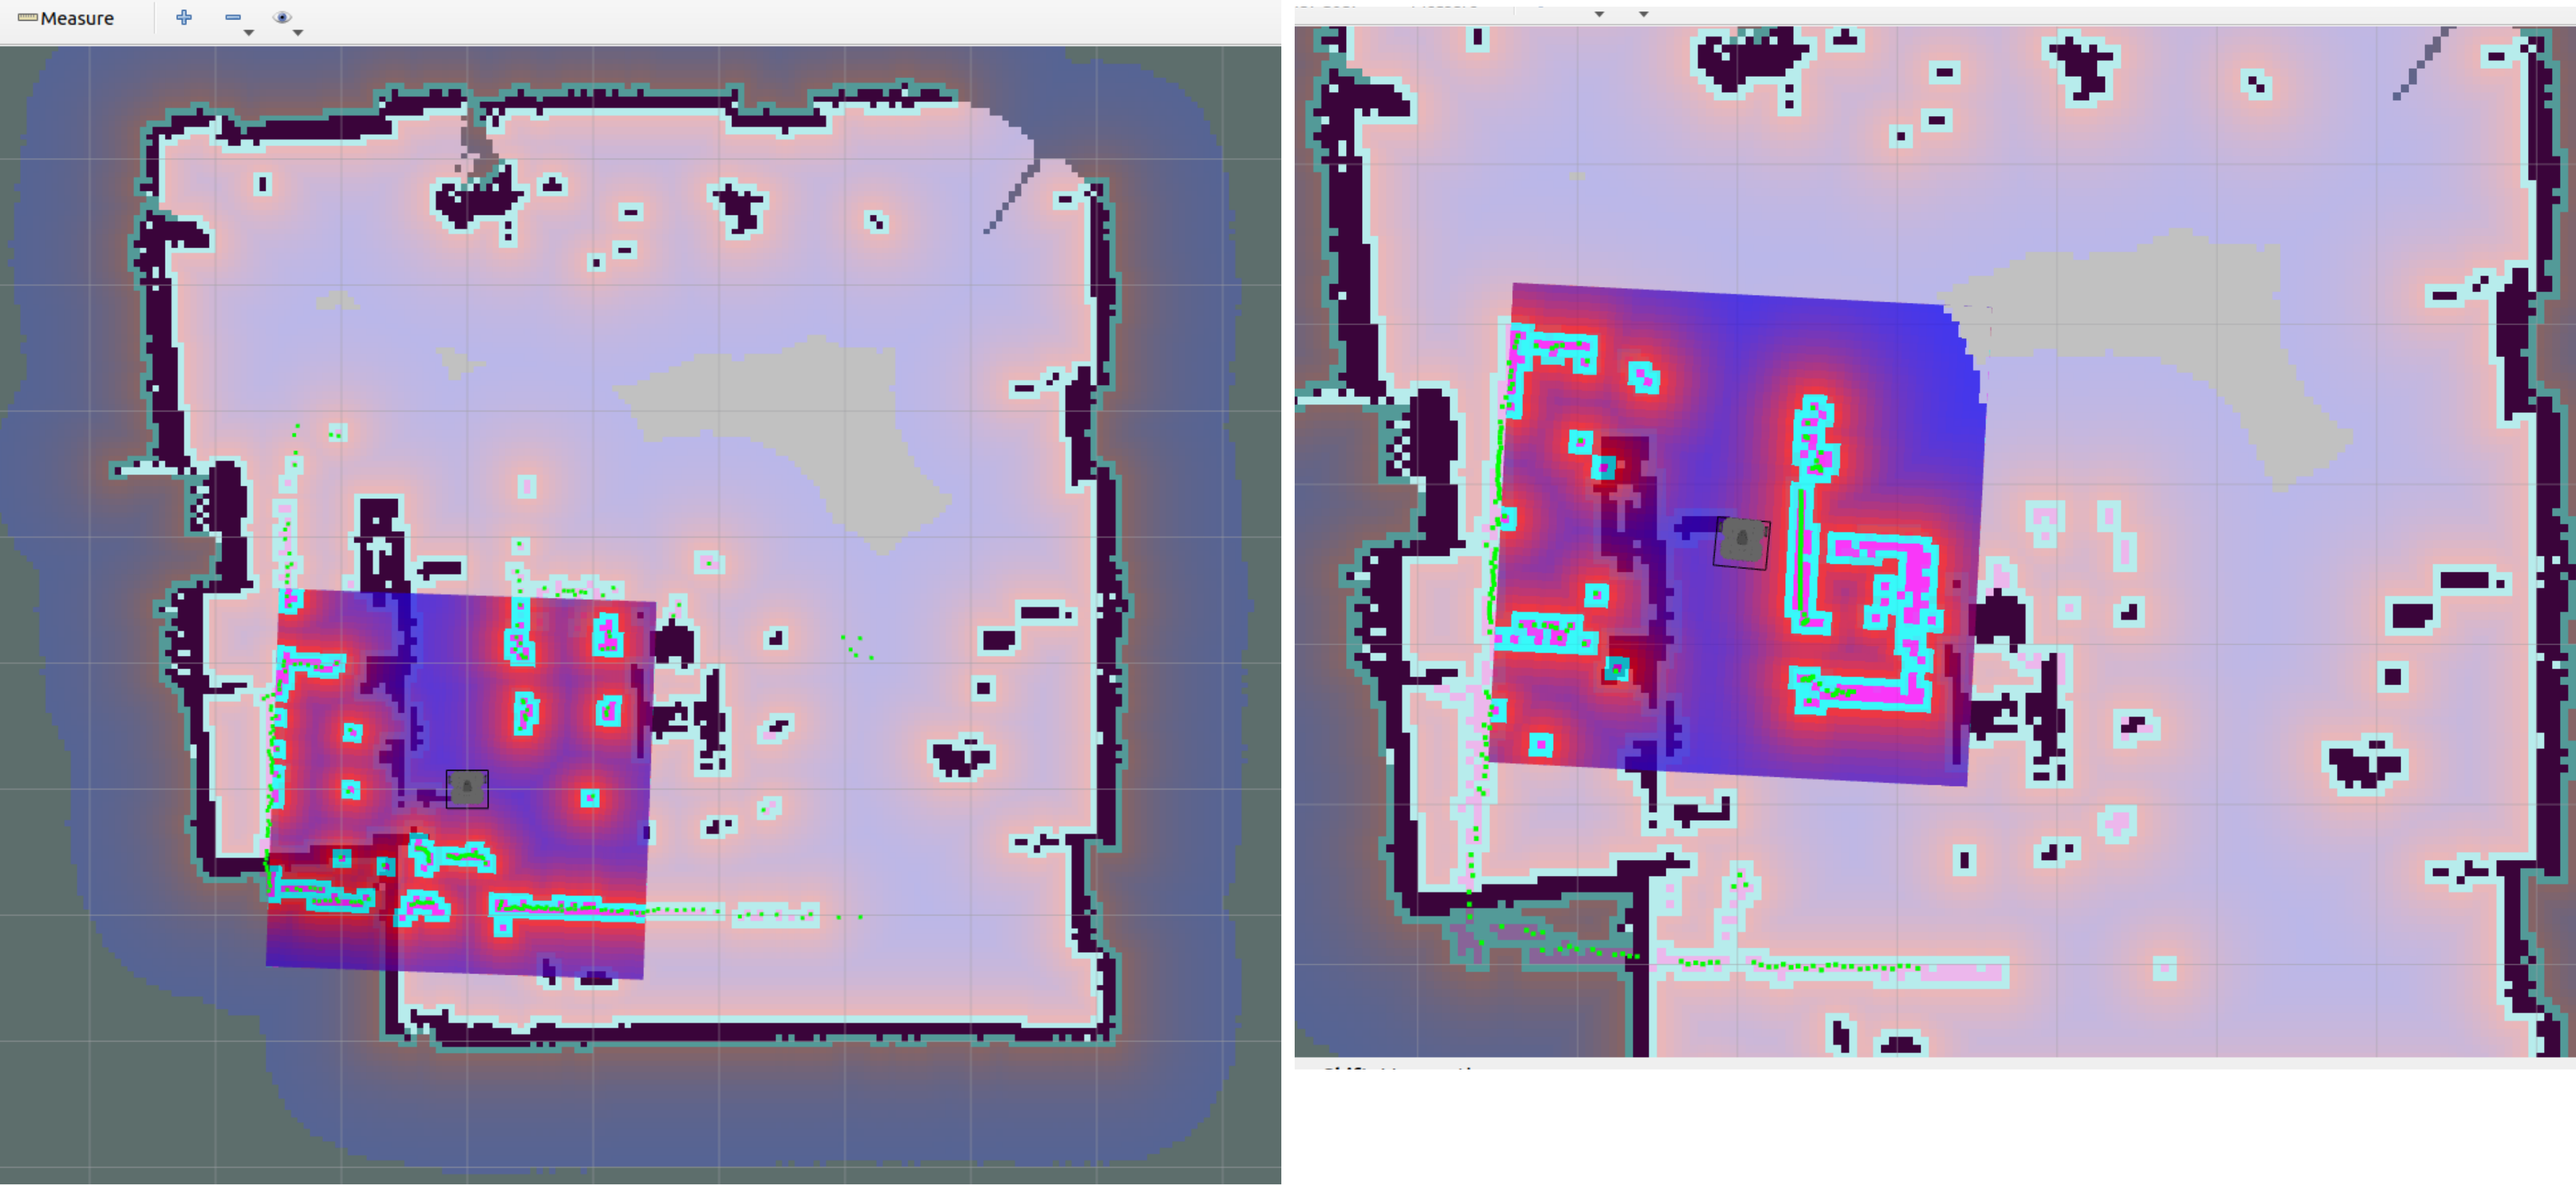
\includegraphics[width=1\linewidth]{amcl-lab-rosbag-1-1-1-1.png}
    \caption{AMCL iteration, with wrong initial position (x:1, y:1), and default number of particles ([1-1])}
    \label{fig:amcl-lab-rosbag-1-1-1-1}
\end{figure}
% If Printing on DOUBLE SIDED pages, the second page should be white.
% Otherwise, comment the following command:
\cleardoublepage
%
%Chapter 4
% #############################################################################
% This is Chapter 4
% !TEX root = ../main.tex
% #############################################################################
% Change the Name of the Chapter i the following line
\fancychapter{This is the Fourth Chapter}
\cleardoublepage
% The following line allows to ref this chapter
\label{chap:implement}

Aliquam aliquet, est a ullamcorper condimentum, tellus nulla fringilla elit, a iaculis nulla turpis sed wisi. Fusce volutpat. Etiam sodales ante id nunc. Proin ornare dignissim lacus. Nunc porttitor nunc a sem. Sed sollicitudin velit eu magna. Aliquam erat volutpat. Vivamus ornare est non wisi. Proin vel quam. Vivamus egestas. Nunc tempor diam vehicula mauris. Nullam sapien eros, facilisis vel, eleifend non, auctor dapibus, pede. 
% #############################################################################
\section{Development Process}
Suspendisse vestibulum dignissim quam. Integer vel augue. Phasellus nulla purus, interdum ac, venenatis non, varius rutrum, leo. Pellentesque habitant morbi tristique senectus et netus et malesuada fames ac turpis egestas. Duis a eros. Class aptent taciti sociosqu ad litora torquent per conubia nostra, per inceptos hymenaeos. Fusce magna mi, porttitor quis, convallis eget, sodales ac, urna. Phasellus luctus venenatis magna. Vivamus eget lacus. Nunc tincidunt convallis tortor. Duis eros mi, dictum vel, fringilla sit amet, fermentum id, sem. Phasellus nunc enim, faucibus ut, laoreet in, consequat id, metus. Vivamus dignissim. Cras lobortis tempor velit. Phasellus nec diam ac nisl lacinia tristique. Nullam nec metus id mi dictum dignissim. Nullam quis wisi non sem lobortis condimentum. Phasellus pulvinar, nulla non aliquam eleifend, tortor wisi scelerisque felis, in sollicitudin arcu ante lacinia leo.:

\begin{itemize}
\item{Technology Research and Related Works}
\item{Requirements Gathering and Study}
\item{Design of the Architecture}
\item{Implementation Process}
\item{Testing and Functional Validation}
\end{itemize}

Pellentesque nibh felis, eleifend id, commodo in, interdum vitae, leo. Praesent eu elit. Ut eu ligula. Class aptent taciti sociosqu ad litora torquent per conubia nostra, per inceptos hymenaeos. Maecenas elementum augue nec nisl. Proin auctor lorem at nibh. Curabitur nulla purus, feugiat id, elementum in, lobortis quis, pede. Vivamus sodales adipiscing sapien. Vestibulum posuere nulla eget wisi. Integer volutpat ligula eget enim. Suspendisse vitae arcu. Quisque pellentesque. Nullam consequat, sem vitae rhoncus tristique, mauris nulla fermentum est, bibendum ullamcorper sapien magna et quam. Sed dapibus vehicula odio. Proin bibendum gravida nisl. Fusce lorem. Phasellus sagittis, nulla in hendrerit laoreet, libero lacus feugiat urna, eget hendrerit pede magna vitae lorem. Praesent mauris.
% #############################################################################
\section{Development Environment}
Cras sed ante. Phasellus in massa. Curabitur dolor eros, gravida et, hendrerit ac, cursus non, massa. Aliquam lorem. In hac habitasse platea dictumst. Cras eu mauris \Cref{time_control_algorithm}\todo[color=cyan!40, author=RC, fancyline]{Notice the reference to the Algorithm construct}{}. Quisque lacus. Donec ipsum. Nullam vitae sem at nunc pharetra ultricies. Vivamus elit eros, ullamcorper a, adipiscing sit amet, porttitor ut, nibh. 

\begin{algorithm}[ht]
\DontPrintSemicolon
\Begin{
$nextBitrate \longleftarrow nextDownloadLevel$\;
$nextBitrate \longleftarrow GetNextBitrate()$\;
$cpuLoad \longleftarrow GetCpuLoad()$\;
$bitrateDelta \longleftarrow getBitrateDelta(currentBitrate, nextBitrate)$\;
\BlankLine
\If{$bitrateDelta > maxThreshold$}{
     $SetBitrate(nextBitrate)$\;
   }
\BlankLine
  \If{$minThreshold < bitrateDelta < maxThreshold$ {\bf and} $numAttemps < 2$}{ 
       $numAttemps \longleftarrow numAttemps + 1$\;
       }{
       \uElseIf{$minThreshold < bitrateDelta < maxThreshold$ {\bf and} $numAttemps = 2$}{
       $numAttemps \longleftarrow 0$\;
       }
       \Else{$SetBitrate(nextBitrate)$}
      }
  \If{$0 < bitrateDelta < minThreshold$ {\bf and} $numAttemps < 3$}{
       $numAttemps \longleftarrow numAttemps + 1$\;
       }{
       \uElseIf{$0 < bitrateDelta < minThreshold$ {\bf and} $numAttemps = 3$}{
       $SetBitrate(nextBitrate)$\;
       }
       }
}
\caption{Time Control Strategy}
\label{time_control_algorithm}
\end{algorithm}


Maecenas adipiscing mollis massa. Nunc ut dui eget nulla venenatis aliquet. Sed luctus posuere justo. Cras vehicula varius turpis. Vivamus eros metus, tristique sit amet, molestie dignissim, malesuada et, urna..
% #############################################################################
\section{Client Application}
Cras sed ante. Phasellus in massa. Curabitur dolor eros, gravida et, hendrerit ac, cursus non, massa. Aliquam lorem. In hac habitasse platea dictumst. Cras eu mauris. Quisque lacus. Donec ipsum. Nullam vitae sem at nunc pharetra ultricies. 

Vivamus elit eros, ullamcorper a, adipiscing sit amet, porttitor ut, nibh. Maecenas adipiscing mollis massa. Nunc ut dui eget nulla venenatis aliquet. Sed luctus posuere justo. Cras vehicula varius turpis. Vivamus eros metus, tristique sit amet, molestie dignissim, malesuada et, urna.

Quisque lacus. Donec ipsum. Nullam vitae sem at nunc pharetra ultricies. Cras vehicula varius turpis.



\begin{minipage}[c]{1.0\textwidth}
%\begin{center}
\centering
\begin{lstlisting}[language = C++, numbers = none, escapechar = !,
    basicstyle = \ttfamily\bfseries, linewidth = .6\linewidth, frame=tb, caption={A listing with a Tikz picture overlayed}, captionpos=b, label=tikzlist] 
 int!
   \tikz[remember picture] \node [] (a) {};
 !puissance!
   \tikz[remember picture] \node [] (b) {};
 !(int x,!
   \tikz[remember picture] \node [] (c){};
 !int n) { 

     int i, p = 1; !\tikz[remember picture] \node [] (d){};!           

     for (i = 1; i <= n; i++) 
       p = p * x; !\tikz[remember picture] \node [inner xsep = 40pt] (e){};! 

     return p; !
       \tikz[remember picture] \node [] (f){};!  
 }
\end{lstlisting}

\begin{tikzpicture}[remember picture, overlay,
    every edge/.append style = { ->, thick, >=stealth,
                                  darkgray, dashed, line width = 1pt },
    every node/.append style = { align = center, minimum height = 10pt,
                                 font = \bfseries, fill= green!20},
                  text width = 2.5cm ]
  \node [above left = .75cm and -.75 cm of a,text width = 2.2cm]
                             (A) {return value type};
  \node [right = 0.25cm of A, text width = 1.9cm]
                             (B) {function name};
  \node [right = 0.5cm of B] (C) {list of formal parameters};
  \node [right = 4.cm of d]  (D) {local variables declaration};
  \node [right = 2.cm of e]  (E) {instructions};
  \node [right = 5.cm of f]  (F) {instruction \texttt{\bfseries return}};  
  \draw (A.south) + (0, 0) coordinate(x1) edge (x1|-a.north);
  \draw (B.south) + (0, 0) coordinate(x2) edge (x2|-b.north);
  \draw (C.south) + (0, 0) coordinate(x3) edge (x3|-c.north);
  \draw (D.west) edge (d.east) ;
  \draw (E.west) edge (e.east) ;  
  \draw (F.west) edge (f.east) ;
\end{tikzpicture}
%\end{center}
\end{minipage}

\textcolor{violet}{And here another method (\Cref{tikzlist}) for mixing (overlay) a picture with a listing of code.}
% #############################################################################
\subsection{User Interface}
Donec semper turpis sed diam. Sed consequat ligula nec tortor. Integer eget sem. Ut vitae enim eu est vehicula gravida. Morbi ipsum ipsum, porta nec, tempor id, auctor vitae, purus. Pellentesque neque. Nulla luctus erat vitae libero. Integer nec enim. Phasellus aliquam enim et tortor. Quisque aliquet, quam elementum condimentum feugiat, tellus odio consectetuer wisi, vel nonummy sem neque in elit. Curabitur eleifend wisi iaculis ipsum. Pellentesque habitant morbi tristique senectus et netus et malesuada fames ac turpis egestas. In non velit non ligula laoreet ultrices. Praesent ultricies facilisis nisl. Vivamus luctus elit sit amet mi. Phasellus pellentesque, erat eget elementum volutpat, dolor nisl porta neque, vitae sodales ipsum nibh in ligula. Maecenas mattis pulvinar diam. Curabitur sed leo..

Cras eu mauris. Quisque lacus. Donec ipsum. Nullam vitae sem at nunc pharetra ultricies. Vivamus elit eros, ullamcorper a, adipiscing sit amet, porttitor ut, nibh. Maecenas adipiscing mollis massa. Nunc ut dui eget nulla venenatis aliquet. Sed luctus posuere justo. Cras vehicula varius turpis. 
% #############################################################################
\subsection{Vivamus luctus elit sit amet mi}
Nulla facilisi. In vel sem. Morbi id urna in diam dignissim feugiat. Proin molestie tortor eu velit. Aliquam erat volutpat. Nullam ultrices, diam tempus vulputate egestas, eros pede varius leo, sed imperdiet lectus est ornare odio. Lorem ipsum dolor sit amet, consectetuer adipiscing elit. Proin consectetuer velit in dui. Phasellus wisi purus, interdum vitae, rutrum accumsan, viverra in, velit. Sed enim risus, congue non, tristique in, commodo eu, metus. Aenean tortor mi, imperdiet id, gravida eu, posuere eu, felis. 

Mauris sollicitudin, turpis in hendrerit sodales, lectus ipsum pellentesque ligula, sit amet scelerisque urna nibh ut arcu. Aliquam in lacus. 

\Cref{fig:ui_playout,fig:ui_loading}\todo[color=cyan!40, author=RC, fancyline]{A figure with Subfigures}{} proin at eros non eros adipiscing mollis.

\begin{figure}[htbp]
	\centering
	\subfigure[Media Loading Window]{\label{fig:ui_loading} 		\includegraphics[width=0.3\textwidth]{./Images/ui_loading}} \qquad
	\subfigure[Play-out Session UI]{\label{fig:ui_playout}
		\includegraphics[width=0.3\textwidth]{./Images/ui_playout}}
	\caption{Complete User Interface}
	\label{fig:user_interface}
\end{figure}

Vestibulum ante ipsum primis in \ac{UI} faucibus orci luctus et ultrices posuere cubilia Curae; Nulla placerat aliquam wisi. Mauris viverra odio. Quisque fermentum pulvinar odio. Proin posuere est vitae ligula. Etiam euismod. Cras a eros.
% If Printing on DOUBLE SIDED pages, the second page should be white.
% Otherwise, comment the following command:
%\cleardoublepage
%
%Chapter 5
% #############################################################################
% This is Chapter 5
% !TEX root = ../main.tex
% #############################################################################
% Change the Name of the Chapter i the following line
\fancychapter{This is the Fifth Chapter}
\cleardoublepage
% The following line allows to ref this chapter
\label{chap:evaluation}

Lorem ipsum dolor sit amet, consectetuer adipiscing elit. Morbi commodo, ipsum sed pharetra gravida, orci magna rhoncus neque, id pulvinar odio lorem non turpis. Nullam sit amet enim. Suspendisse id velit vitae ligula volutpat condimentum. Aliquam erat volutpat. Sed quis velit. Nulla facilisi. Nulla libero. Vivamus pharetra posuere sapien. Nam consectetuer. Sed aliquam, nunc eget euismod ullamcorper, lectus nunc ullamcorper orci, fermentum bibendum enim nibh eget ipsum. Donec porttitor ligula eu dolor. Maecenas vitae nulla consequat libero cursus venenatis. Nam magna enim, accumsan eu, blandit sed, blandit a, eros. 
% #############################################################################
\section{Maecenas vitae nulla consequat} 
Aliquam aliquet, est a ullamcorper condimentum, tellus nulla fringilla elit, a iaculis nulla turpis sed wisi. Fusce volutpat. Etiam sodales ante id nunc. Proin ornare dignissim lacus. Nunc porttitor nunc a sem. Sed sollicitudin velit eu magna. Aliquam erat volutpat. Vivamus ornare est non wisi. Proin vel quam. Vivamus egestas. Nunc tempor diam vehicula mauris. Nullam sapien eros \Cref{fig:test_env}, facilisis vel, eleifend non, auctor dapibus, pede.

\begin{figure}[h]
\centering
\includegraphics[width=0.8\textwidth]{./Images/test_env}
\caption{Test Environment}
\label{fig:test_env}
\end{figure}

Aliquam aliquet, est a ullamcorper condimentum, tellus nulla fringilla elit, a iaculis nulla turpis sed wisi. Fusce volutpat. Etiam sodales ante id nunc. Proin ornare dignissim lacus. Nunc porttitor nunc a sem. Sed sollicitudin velit eu magna. Aliquam erat volutpat. Vivamus egestas. Nunc tempor diam vehicula mauris. Nullam sapien eros, facilisis vel, eleifend non, auctor dapibus, pede \Cref{tab:network_profiles} used in the tests. The Network Link Conditioner allows to force/simulate fluctuations in fixed network segments.

\begin{table}[htb]
\centering
\normalsize
    \caption{Network Link Conditioner Profiles}
    \label{tab:network_profiles}
{\footnotesize
    \begin{tabular}{ | c | c | c | c | }
    \hline 
    \textbf{Network Profile}	& \textbf{Bandwidth} & \textbf{Packets Droped} & \textbf{Delay}\\ \hline \hline
    Wifi  & 40 mbps  &  0\%  &   1 ms \\ \hline
    3G  & 780 kbps  &  0\%  &   100 ms \\ \hline 
    Edge  & 240 kbps  &  0\%  &   400 ms \\ \hline
    \end{tabular}
    }
\end{table}

Aliquam aliquet, est a ullamcorper condimentum, tellus nulla fringilla elit, a iaculis nulla turpis sed wisi. Fusce volutpat. Etiam sodales ante id nunc. Proin ornare dignissim lacus. Nunc porttitor nunc a sem. Sed sollicitudin velit eu magna. Aliquam erat volutpat. Vivamus ornare est non wisi. Proin vel quam. Vivamus egestas. Nunc tempor diam vehicula mauris. Nullam sapien eros, facilisis vel, eleifend non, auctor dapibus, pede.
% #############################################################################
\section{Proin ornare dignissim lacus}
Pellentesque habitant morbi tristique senectus et netus et malesuada fames ac turpis egestas. Vestibulum tortor quam, feugiat vitae, ultricies eget, tempor sit amet, ante. Donec eu libero sit amet quam egestas semper. Aenean ultricies mi vitae est. Mauris placerat eleifend leo. Quisque sit amet est et sapien ullamcorper pharetra. Vestibulum erat wisi, condimentum sed, commodo vitae, ornare sit amet, wisi. Aenean fermentum, elit eget tincidunt condimentum, eros ipsum rutrum orci, sagittis tempus lacus enim ac dui. Donec non enim in turpis pulvinar facilisis. Ut felis.

Et ``optimistic'' nulla dui purus, eleifend vel, consequat non, dictum porta, nulla. Duis ante mi, laoreet ut, commodo eleifend, cursus nec, lorem. Aenean eu est. Etiam imperdiet turpis. Praesent nec augue. Curabitur ligula quam, rutrum id, tempor sed, consequat ac, dui $G_j$, nec ligula et lorem consequat ullamcorper $p$ ut mauris eu mi mollis luctus $j$, porttitor ut, \Cref{unchoke_gain}, uctus posuere justo:

\begin{description}
  \item[$N_j$] Is the number of times peer $j$ has been optimistically unchoked.
  \item[$n_j$] Among the $N_j$ unchokes, the number of times that peer $j$ responded with unchoke or supplied segments to peer $p$.
  \item[$C_{r[j]}$] The cooperation ratio of peer $j$. If peer $j$ never supplied peer $p$, the information of $C_{r[j]}$ may not be available.
  \item[$C_{r (max)}$] The maximum cooperation ratio of peer $p$’s neighbors, i.e., $C_{r (max)} = max(C_r)$.
\end{description}

\begin{equation}
\label{unchoke_gain}
 G_j =
  \begin{dcases}
    \frac{n_j C_{r[j]}}{N_j} &\quad \text{if } n_j > 0\\
    \frac{C_{r (max)}}{N_j + 1} &\quad \text{if } n_j = 0
  \end{dcases}
\end{equation}

Cursus $C_{r (max)}$ conubia nostra, per inceptos hymenaeos $j$ gadipiscing mollis massa $N_j = 0$, unc ut dui eget nulla venenatis aliquet $G_j = C_{r (max)}$.

Vestibulum accumsan eros nec magna. Vestibulum vitae dui. Vestibulum nec ligula et lorem consequat ullamcorper. Class aptent taciti sociosqu ad litora torquent per conubia nostra, per inceptos hymenaeos. Phasellus eget nisl ut elit porta ullamcorper. Maecenas tincidunt velit quis orci. Sed in dui. Nullam ut mauris eu mi mollis luctus. Class aptent taciti sociosqu ad litora torquent per conubia nostra, per inceptos hymenaeos. Sed cursus cursus velit. Sed a massa. 

Both \Cref{fig:tx_layer_4,fig:tx_layer_5} Phasellus eget nisl ut elit porta ``perfect'' tincidunt. Class aptent taciti sociosqu ad litora torquent per conubia nostra.

\begin{figure}[h]
%\centering
       \subfigure[Adaptation System Test 4]{\label{fig:tx_layer_4}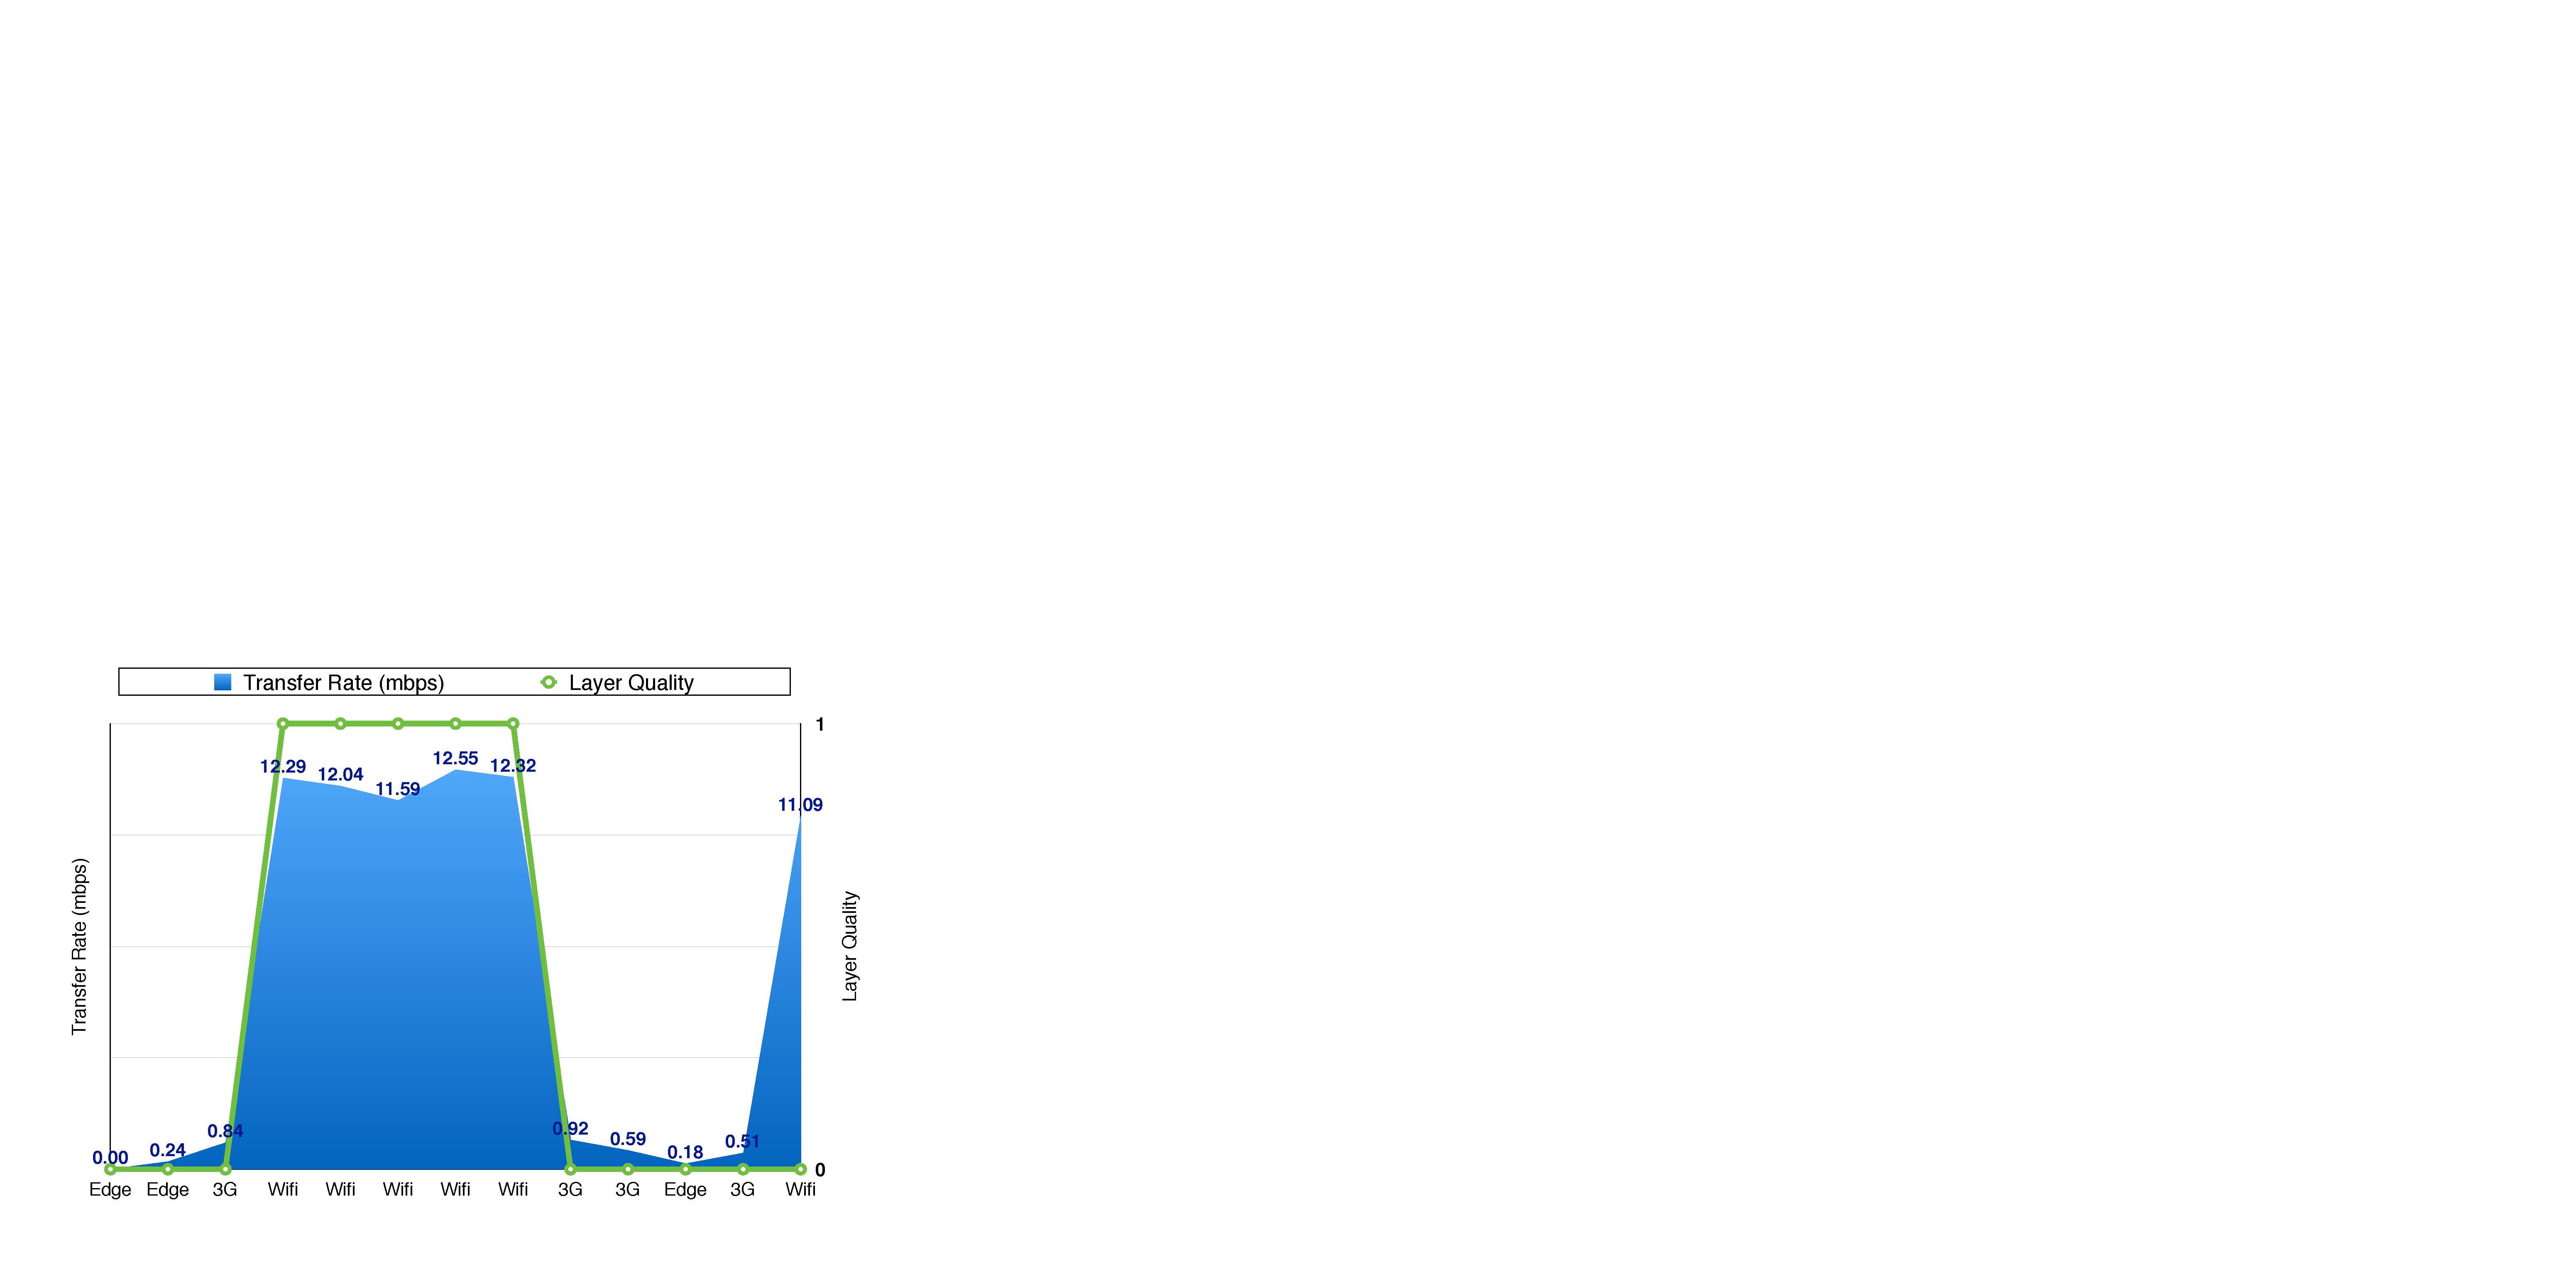
\includegraphics[width=0.5\textwidth]{./Images/tx_layer_4}}  
   %    \centering 
       \subfigure[Adaptation System Test 5]{\label{fig:tx_layer_5}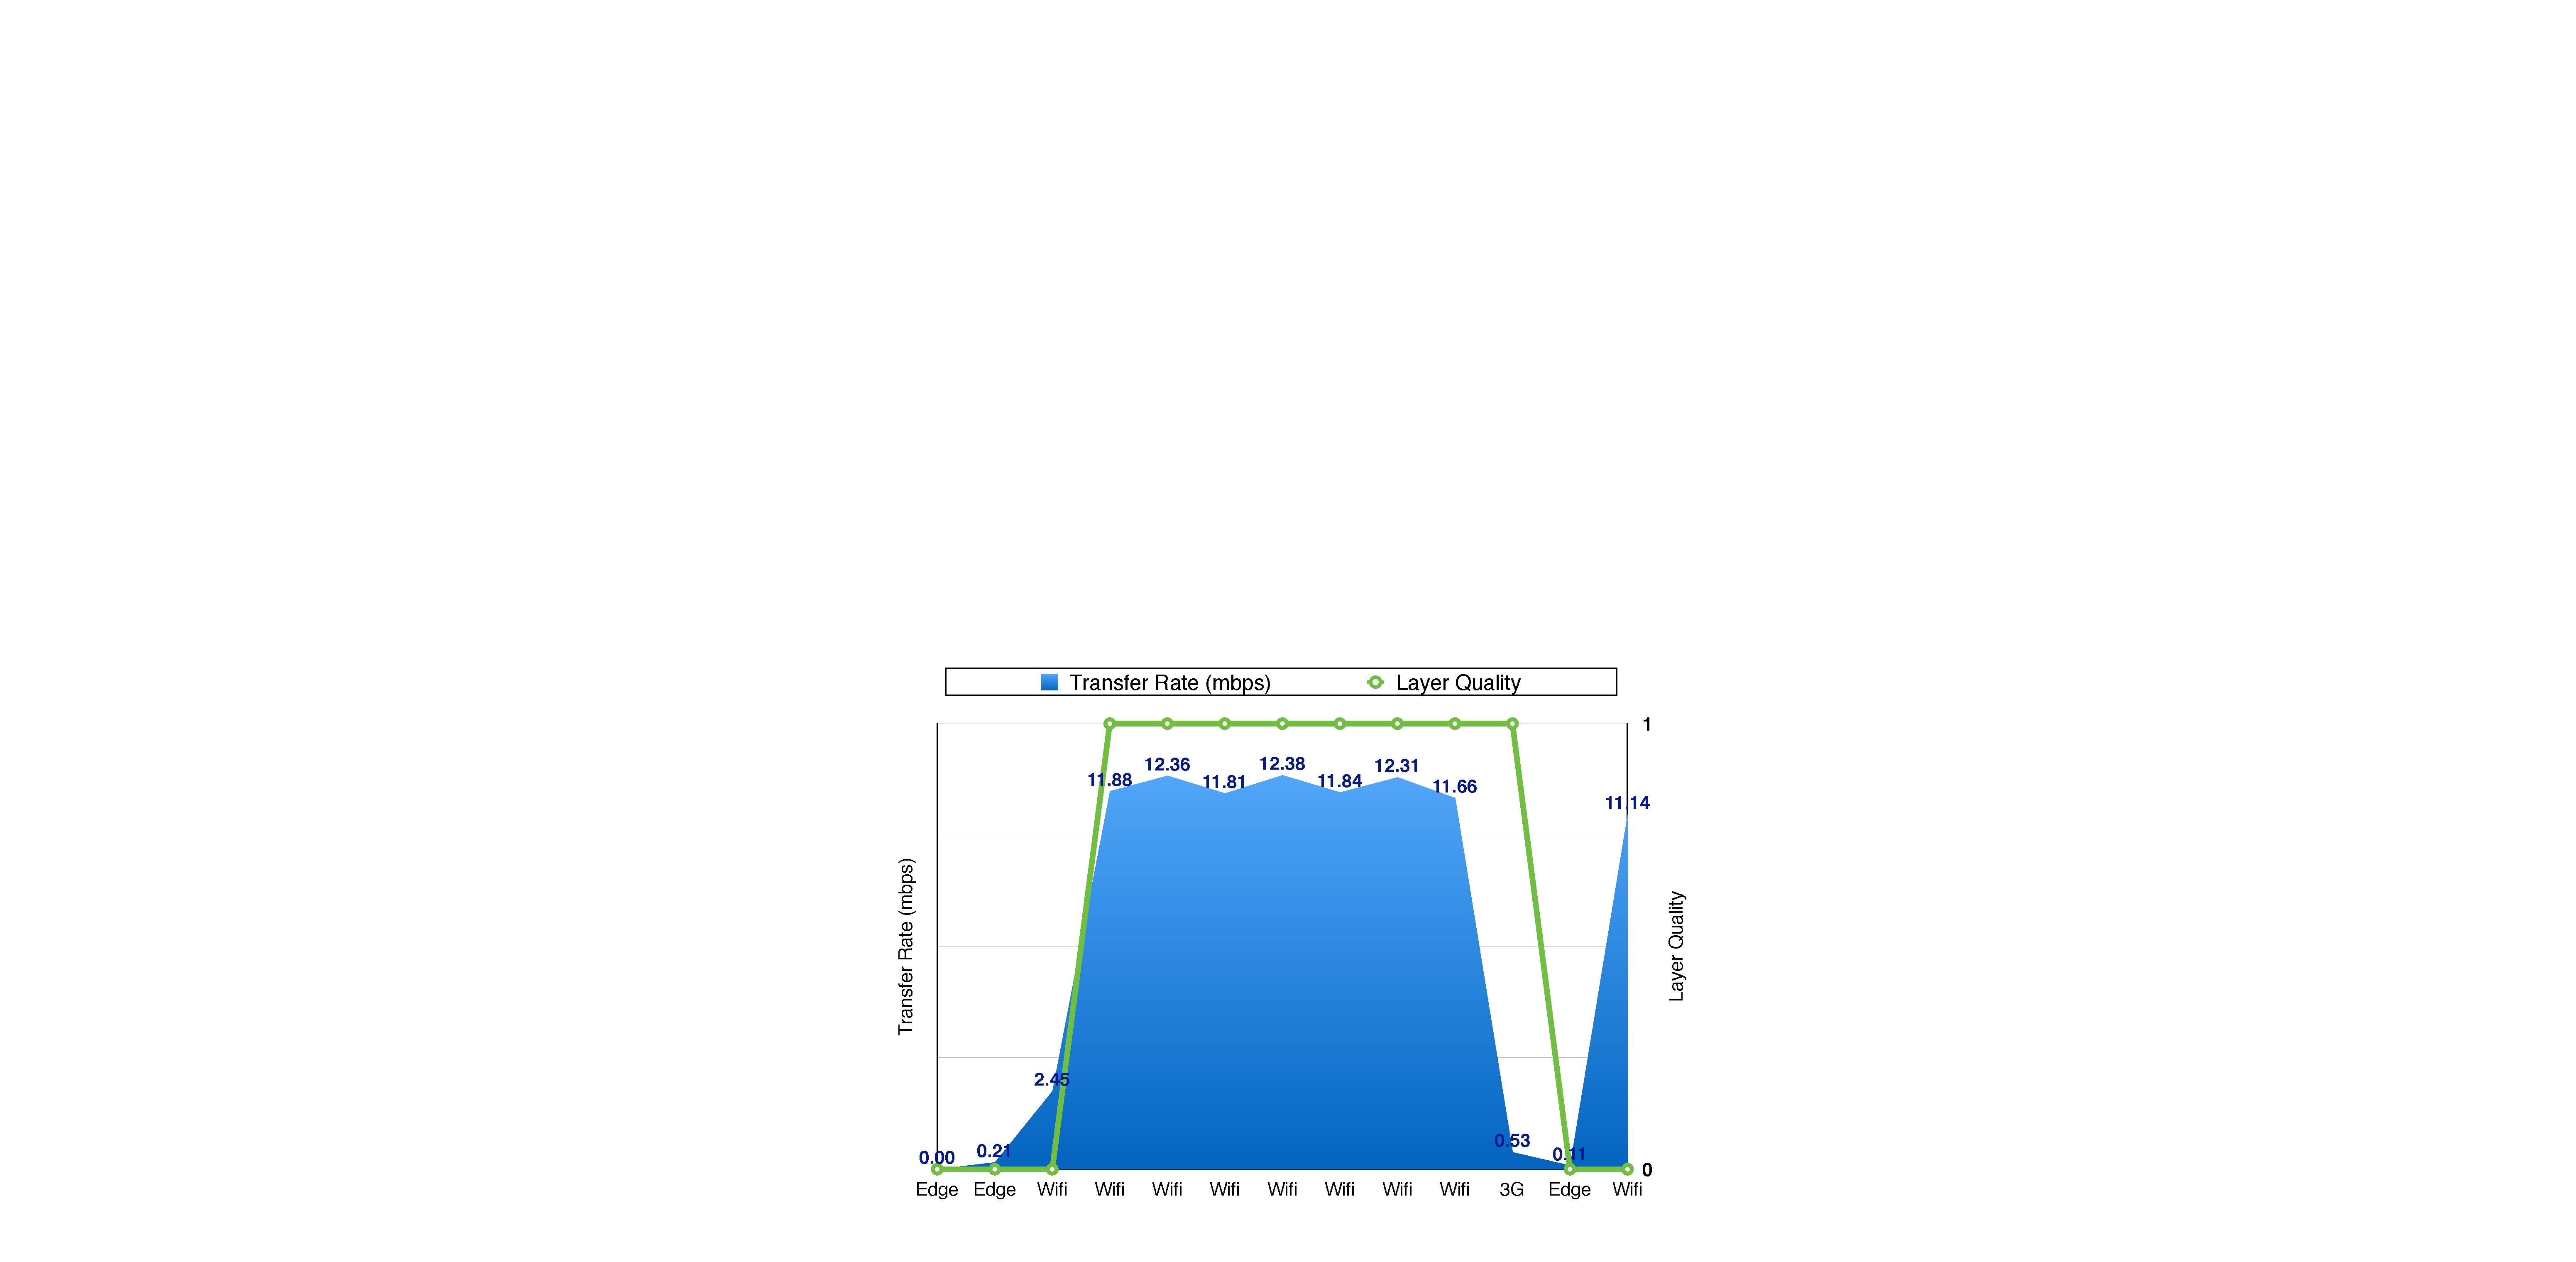
\includegraphics[width=0.5\textwidth]{./Images/tx_layer_5}}   
        \caption{Adaptation System Behavior Test}
        \label{fig:fig:adapt_behave_2}
\end{figure}

Cras sed ante. Phasellus in massa. Curabitur dolor eros, gravida et, hendrerit ac, cursus non, massa. Aliquam lorem. In hac habitasse platea dictumst. Cras eu mauris. Quisque lacus. Donec ipsum. Nullam vitae sem at nunc pharetra ultricies. Vivamus elit eros, ullamcorper a, adipiscing sit amet, porttitor ut, nibh. Maecenas adipiscing mollis massa. Nunc ut dui eget nulla venenatis aliquet. Sed luctus posuere justo. Cras vehicula varius turpis. Vivamus eros metus, tristique sit amet, molestie dignissim, malesuada et, urna.
% If Printing on DOUBLE SIDED pages, the second page should be white.
% Otherwise, comment the following command:
\cleardoublepage
%
%Chapter 6
% #############################################################################
% This is Chapter 6
% !TEX root = ../main.tex
% #############################################################################
% Change the Name of the Chapter i the following line
\fancychapter{Conclusion}
\cleardoublepage
% The following line allows to ref this chapter
\label{chap:conclusion}

 Pellentesque vel dui sed orci faucibus iaculis. Suspendisse dictum magna id purus tincidunt rutrum. Nulla congue. Vivamus sit amet lorem posuere dui vulputate ornare. Phasellus mattis sollicitudin ligula. Duis dignissim felis et urna. Integer adipiscing congue metus\todo[color=green!40, author=Rui Cruz, fancyline]{You should always start a Chapter with an introductory text}{}.
% #############################################################################
\section{Conclusions}
Lorem ipsum dolor sit amet, consectetuer adipiscing elit. Morbi commodo, ipsum sed pharetra gravida, orci magna rhoncus neque, id pulvinar odio lorem non turpis. Nullam sit amet enim. Suspendisse id velit vitae ligula volutpat condimentum. Aliquam erat volutpat. Sed quis velit. Nulla facilisi. Nulla libero. Vivamus pharetra posuere sapien. Nam consectetuer. Sed aliquam, nunc eget euismod ullamcorper, lectus nunc ullamcorper orci, fermentum bibendum enim nibh eget ipsum. Donec porttitor ligula eu dolor. Maecenas vitae nulla consequat libero cursus venenatis. Nam magna enim, accumsan eu, blandit sed, blandit a, eros.

Quisque facilisis erat a dui. Nam malesuada ornare dolor. Cras gravida, diam sit amet rhoncus ornare, erat elit consectetuer erat, id egestas pede nibh eget odio. Proin tincidunt, velit vel porta elementum, magna diam molestie sapien, non aliquet massa pede eu diam. Aliquam iaculis. Fusce et ipsum et nulla tristique facilisis. Donec eget sem sit amet ligula viverra gravida. Etiam vehicula urna vel turpis. Suspendisse sagittis ante a urna. Morbi a est quis orci consequat rutrum. Nullam egestas feugiat felis. Integer adipiscing semper ligula. Nunc molestie, nisl sit amet cursus convallis, sapien lectus pretium metus, vitae pretium enim wisi id lectus. Donec vestibulum. Etiam vel nibh. Nulla facilisi. Mauris pharetra. Donec augue. Fusce ultrices, neque id dignissim ultrices, tellus mauris dictum elit, vel lacinia enim metus eu nunc.

Proin at eros non eros adipiscing mollis. Donec semper turpis sed diam. Sed consequat ligula nec tortor. Integer eget sem. Ut vitae enim eu est vehicula gravida. Morbi ipsum ipsum, porta nec, tempor id, auctor vitae, purus. Pellentesque neque. Nulla luctus erat vitae libero. Integer nec enim. Phasellus aliquam enim et tortor. Quisque aliquet, quam elementum condimentum feugiat, tellus odio consectetuer wisi, vel nonummy sem neque in elit. Curabitur eleifend wisi iaculis ipsum. Pellentesque habitant morbi tristique senectus et netus et malesuada fames ac turpis egestas. In non velit non ligula laoreet ultrices. Praesent ultricies facilisis nisl. Vivamus luctus elit sit amet mi. Phasellus pellentesque, erat eget elementum volutpat, dolor nisl porta neque, vitae sodales ipsum nibh in ligula. Maecenas mattis pulvinar diam. Curabitur sed leo.

Nulla facilisi. In vel sem. Morbi id urna in diam dignissim feugiat. Proin molestie tortor eu velit. Aliquam erat volutpat. Nullam ultrices, diam tempus vulputate egestas, eros pede varius leo, sed imperdiet lectus est ornare odio. Lorem ipsum dolor sit amet, consectetuer adipiscing elit. Proin consectetuer velit in dui. Phasellus wisi purus, interdum vitae, rutrum accumsan, viverra in, velit. Sed enim risus, congue non, tristique in, commodo eu, metus. Aenean tortor mi, imperdiet id, gravida eu, posuere eu, felis. Mauris sollicitudin, turpis in hendrerit sodales, lectus ipsum pellentesque ligula, sit amet scelerisque urna nibh ut arcu. Aliquam in lacus. Vestibulum ante ipsum primis in faucibus orci luctus et ultrices posuere cubilia Curae; Nulla placerat aliquam wisi. Mauris viverra odio. Quisque fermentum pulvinar odio. Proin posuere est vitae ligula. Etiam euismod. Cras a eros.

Nunc auctor bibendum eros. Maecenas porta accumsan mauris. Etiam enim enim, elementum sed, bibendum quis, rhoncus non, metus. Fusce neque dolor, adipiscing sed, consectetuer et, lacinia sit amet, quam.
% #############################################################################
\section{System Limitations and Future Work}
Aliquam aliquet, est a ullamcorper condimentum, tellus nulla fringilla elit, a iaculis nulla turpis sed wisi. Fusce volutpat. Etiam sodales ante id nunc. Proin ornare dignissim lacus. Nunc porttitor nunc a sem. Sed sollicitudin velit eu magna. Aliquam erat volutpat. Vivamus ornare est non wisi. Proin vel quam. Vivamus egestas. Nunc tempor diam vehicula mauris. Nullam sapien eros, facilisis vel, eleifend non, auctor dapibus, pede.
% If Printing on DOUBLE SIDED pages, the second page should be white.
% Otherwise, comment the following command:
\cleardoublepage
%
% -----------------------------------------------------------------------------
% BIBLIOGRAPHY
% Add the Bibliography to the PDF table of contents (not the document table of contents)
%\pdfbookmark[0]{Bibliography}{bib}
\addcontentsline{toc}{chapter}{Bibliography}
% The bibliography style sheet
% Chose your preferences on the format of the entries and the Labels:
% IEEEtran: Used in general (recommended for IST Thesis)
%           Entries are labelled and sorted by appearance in the document
%           Labels are Numeric inside square brackets
\bibliographystyle{IEEEtran}
%
% Apalike:  Entries formatted alphabetically, last name first, with identation
%           Labels with Autor's Name and Year inside square brackets
%\bibliographystyle{apalike}
%
% Alpha:    Entries formatted with Autor's Name and Year, hanging identation
%           Labels with Autor's abbr. Names and Year inside square brackets
%\bibliographystyle{alpha}
%
% Acm:     Entries formatted with Autor's Name (small Caps), hanging identation
%          Labels are Numeric inside square brackets
%\bibliographystyle{acm}
% The following command resets the 'emphasis' style for bibliography entries
\normalem
% Name of your BiBTeX file
\bibliography{./Thesis-MSc-Bibliography} % Put here your own filename
%
% The following command modifies the 'emphasis' style for bibliography entries
\ULforem
% If Printing on DOUBLE SIDED pages, the second page should be white.
% Otherwise, comment the following command:
\cleardoublepage
%
% -----------------------------------------------------------------------------
% HERE GO THE APPENDIXES IF REQUIRED
% If not required just comment the blocks
\appendix
%% First Appendix
%\pdfbookmark[1]{Appendix A}{appendix}
% #############################################################################
% This is Appendix A
% !TEX root = ../main.tex
% #############################################################################
\chapter{Code of Project}
\label{chapter:appendixA}

Nulla dui purus, eleifend vel, consequat non, dictum porta, nulla. Duis ante mi, laoreet ut, commodo eleifend, cursus nec, lorem. Aenean eu est. Etiam imperdiet turpis. Praesent nec augue. Curabitur ligula quam, rutrum id, tempor sed, consequat ac, dui. Vestibulum accumsan eros nec magna. Vestibulum vitae dui. Vestibulum nec ligula et lorem consequat ullamcorper. 

\begin{lstlisting}[frame=lines,style=XML,caption={Example of a XML file.},label=xmlEx]
<?xml version="1.0" encoding="UTF-8"?>
<StreamInfo version="2.0">
    <Clip duration="PT01M0.00S">
        <BaseURL>videos/</BaseURL>
        <Description>svc_1</Description>
        <Representation mimeType="video/SVC" codecs="svc" frameRate="30.00" bandwidth="401.90"
            width="176" height="144" id="L0">
            <BaseURL>svc_1/</BaseURL>
            <SegmentInfo from="0" to="11" duration="PT5.00S">
                <BaseURL>svc_1-L0-</BaseURL>
            </SegmentInfo>
        </Representation>
        <Representation mimeType="video/SVC" codecs="svc" frameRate="30.00" bandwidth="1322.60"
            width="352" height="288" id="L1">
            <BaseURL>svc_1/</BaseURL>
            <SegmentInfo from="0" to="11" duration="PT5.00S">
                <BaseURL>svc_1-L1-</BaseURL>
            </SegmentInfo>
        </Representation>
    </Clip>
</StreamInfo>
\end{lstlisting}

Etiam imperdiet turpis. Praesent nec augue. Curabitur ligula quam, rutrum id, tempor sed, consequat ac, dui. Maecenas tincidunt velit quis orci. Sed in dui. Nullam ut mauris eu mi mollis luctus. Class aptent taciti sociosqu ad litora torquent per conubia nostra, per inceptos hymenaeos. Sed cursus cursus velit. Sed a massa. Duis dignissim euismod quam.

\begin{spacing}{0.5}
\lstinputlisting[style=coloredASM,language=Assembler,numbers=left,caption={Assembler Main Code.},label=code]
{./tables_and_code/example.asm.txt}
\end{spacing}


Class aptent taciti sociosqu ad litora torquent per conubia nostra, per inceptos hymenaeos. Phasellus eget nisl ut elit porta ullamcorper. Maecenas tincidunt velit quis orci. Sed in dui. Nullam ut mauris eu mi mollis luctus. Class aptent taciti sociosqu ad litora torquent per conubia nostra, per inceptos hymenaeos.

This inline MATLAB code \mcode{for i=1:3, disp('cool'); end;} uses the \verb|\mcode{}| command.\footnote{MATLAB Works also in footnotes: \mcodefn{for i=1:3, disp('cool'); end;}}

Nullam ut mauris eu mi mollis luctus. Class aptent taciti sociosqu ad litora torquent per conubia nostra, per inceptos hymenaeos. Sed cursus cursus velit. Sed a massa. Duis dignissim euismod quam. Nullam euismod metus ut orci.

\begin{lstlisting}[language=matlabfloz,caption={\mcode{Matlab Function}}]
for i = 1:3
	if i >= 5 && a ~= b       % literate programming replacement
		disp('cool');         % comment with some §\mcommentfont\LaTeX in it: $\mcommentfont\pi x^2$§
	end
	[:,ind] = max(vec);
	x_last = x(1,end) - 1;
	v(end);
	ylabel('Voltage (µV)');
end
\end{lstlisting}

Nullam ut mauris eu mi mollis luctus. Class aptent taciti sociosqu ad litora torquent per conubia nostra, per inceptos hymenaeos. Sed cursus cursus velit. Sed a massa. Duis dignissim euismod quam. Nullam euismod metus ut orci.

\lstinputlisting[
	label=lst:matlab_code,
	caption={\mcode{function.m}},
	breaklines=true
	]{./tables_and_code/function.m}

Class aptent taciti sociosqu ad litora torquent per conubia nostra, per inceptos hymenaeos. Phasellus eget nisl ut elit porta ullamcorper. Maecenas tincidunt velit quis orci. Sed in dui. Nullam ut mauris eu mi mollis luctus. Class aptent taciti sociosqu ad litora torquent per conubia nostra, per inceptos hymenaeos. Sed cursus cursus velit. Sed a massa. Duis dignissim euismod quam. Nullam euismod metus ut orci. Vestibulum erat libero, scelerisque et, porttitor et, varius a, leo.

\begin{lstlisting}[style=htmlcssjs,caption={HTML with CSS Code}]
<!DOCTYPE html>
<html>
  <head>
    <title>Listings Style Test</title>
    <meta charset="UTF-8">
    <style>
      /* CSS Test */
      * {
        padding: 0;
        border: 0;
        margin: 0;
      }
    </style>
    <link rel="stylesheet" href="css/style.css" />
  </head>
  <header> hey </header>
  <article> this is a article </article>
  <body>
    <!-- Paragraphs are fine -->
    <div id="box">			
			<p>
			  Hello World
			</p>
      <p>Hello World</p>
      <p id="test">Hello World</p>
			<p></p>
    </div>
    <div>Test</div>
    <!-- HTML script is not consistent -->
    <script src="js/benchmark.js"></script>
    <script>
      function createSquare(x, y) {
        // This is a comment.
        var square = document.createElement('div');
        square.style.width = square.style.height = '50px';
        square.style.backgroundColor = 'blue';
        
        /*
         * This is another comment.
         */
        square.style.position = 'absolute';
        square.style.left = x + 'px'; 
        square.style.top = y + 'px';
        
        var body = document.getElementsByTagName('body')[0];
        body.appendChild(square);
      };
      
      // Please take a look at +=
      window.addEventListener('mousedown', function(event) {
        // German umlaut test: Berührungspunkt ermitteln
        var x = event.touches[0].pageX;
        var y = event.touches[0].pageY;
        var lookAtThis += 1;
      });
    </script>
  </body>
</html>
\end{lstlisting}

Nulla dui purus, eleifend vel, consequat non, dictum porta, nulla. Duis ante mi, laoreet ut, commodo eleifend, cursus nec, lorem. Aenean eu est. Etiam imperdiet turpis. Praesent nec augue. Curabitur ligula quam, rutrum id, tempor sed, consequat ac, dui. Vestibulum accumsan eros nec magna. Vestibulum vitae dui. Vestibulum nec ligula et lorem consequat ullamcorper.

\begin{lstlisting}[style=htmlcssjs,caption={HTML CSS Javascript Code}]

@media only screen and (min-width: 768px) and (max-width: 991px) {
	
	#main {
		width: 712px;
		padding: 100px 28px 120px;
	}
	
	/* .mono {
		font-size: 90%;
	} */
	
	.cssbtn a {
		margin-top: 10px;
		margin-bottom: 10px;
		width: 60px;  
		height: 60px;   
		font-size: 28px;
		line-height: 62px;
	}
\end{lstlisting}

Nulla dui purus, eleifend vel, consequat non, dictum porta, nulla. Duis ante mi, laoreet ut, commodo eleifend, cursus nec, lorem. Aenean eu est. Etiam imperdiet turpis. Praesent nec augue. Curabitur ligula quam, rutrum id, tempor sed, consequat ac, dui. Vestibulum accumsan eros nec magna. Vestibulum vitae dui. Vestibulum nec ligula et lorem consequat ullamcorper.

\begin{lstlisting} [style=py,caption={PYTHON Code}]
class TelgramRequestHandler(object):
    def handle(self):
        addr = self.client_address[0]         # Client IP-adress
        telgram = self.request.recv(1024)     # Recieve telgram
        print "From: %s, Received: %s" % (addr, telgram)
        return
\end{lstlisting}
%% If Printing on DOUBLE SIDED pages, the second page should be white.
%% Otherwise, comment the following command:
\cleardoublepage
%% Second Appendix
%\pdfbookmark[1]{Appendix B}{appendix}
% #############################################################################
% This is Appendix B
% !TEX root = ../main.tex
% #############################################################################
\chapter{A Large Table}
\label{chapter:appendixB}

Aliquam et nisl vel ligula consectetuer suscipit. Morbi euismod enim eget neque. Donec sagittis massa. Vestibulum quis augue sit amet ipsum laoreet pretium. Nulla facilisi. Duis tincidunt, felis et luctus placerat, ipsum libero vestibulum sem, vitae elementum wisi ipsum a metus. Nulla a enim sed dui hendrerit lobortis. Donec lacinia vulputate magna. Vivamus suscipit lectus at quam. In lectus est, viverra a, ultricies ut, pulvinar vitae, tellus. Donec et lectus et sem rutrum sodales. Morbi cursus. Aliquam a odio. Sed tortor velit, convallis eget, porta interdum, convallis sed, tortor. Phasellus ac libero a lorem auctor mattis. Lorem ipsum dolor sit amet, consectetuer adipiscing elit.

Nunc auctor bibendum eros. Maecenas porta accumsan mauris. Etiam enim enim, elementum sed, bibendum quis, rhoncus non, metus. Fusce neque dolor, adipiscing sed, consectetuer et, lacinia sit amet, quam. Suspendisse wisi quam, consectetuer in, blandit sed, suscipit eu, eros. Etiam ligula enim, tempor ut, blandit nec, mollis eu, lectus. Nam cursus. Vivamus iaculis. Aenean risus purus, pharetra in, blandit quis, gravida a, turpis. Donec nisl. Aenean eget mi. Fusce mattis est id diam. Phasellus faucibus interdum sapien. Duis quis nunc. Sed enim.
Nunc auctor bibendum eros. Maecenas porta accumsan mauris. Etiam enim enim, elementum sed, bibendum quis, rhoncus non, metus. Fusce neque dolor, adipiscing sed, consectetuer et, lacinia sit amet, quam.

% Table Example
\newcommand{\greyrow}{\rowcolor[rgb]{0.9,0.9,0.9}}
\newcommand{\whiterow}{\rowcolor[rgb]{1,1,1}}
\newcommand{\greycell}[1]{\multicolumn{1}{{>{\columncolor[rgb]{0.9,0.9,0.9}}c}}{#1}}
\newcommand{\lightgreycell}[1]{\multicolumn{1}{{>{\columncolor[rgb]{0.9,0.9,0.9}}c}}{#1}}
\newcommand{\mediumgreycell}[1]{\multicolumn{1}{{>{\columncolor[rgb]{0.8,0.8,0.8}}c}}{#1}}
\newcommand{\darkgreycell}[1]{\multicolumn{1}{{>{\columncolor[rgb]{0.7,0.7,0.7}}c}}{#1}}
\newcommand{\whitecell}[1]{\multicolumn{1}{{>{\columncolor[rgb]{1,1,1}}c}}{#1}}

\newcommand{\cellformatG}[1]{\multicolumn{1}{{>{\columncolor[rgb]{.9,.9,.9}}c}}{#1}}
\newcommand{\cellformatW}[1]{\multicolumn{1}{{>{\columncolor[rgb]{1,1,1}}c}}{#1}}
\newcommand{\cellformatlG}[1]{\multicolumn{1}{{|>{\columncolor[rgb]{.9,.9,.9}}c}}{#1}}
\newcommand{\cellformatlW}[1]{\multicolumn{1}{{|>{\columncolor[rgb]{1,1,1}}c}}{#1}}
\newcommand{\cellformatrG}[1]{\multicolumn{1}{{>{\columncolor[rgb]{.9,.9,.9}}c|}}{#1}}
\newcommand{\cellformatrW}[1]{\multicolumn{1}{{>{\columncolor[rgb]{1,1,1}}c|}}{#1}}
\newcommand{\cellformatlrG}[1]{\multicolumn{1}{{|>{\columncolor[rgb]{.9,.9,.9}}c|}}{#1}}
\newcommand{\cellformatlrW}[1]{\multicolumn{1}{{|>{\columncolor[rgb]{1,1,1}}c|}}{#1}}

\begin{table}[t]
\centering
\caption{Example table}
\label{table:table1}
\begin{tabular}{c c c c c c}
\hline
\cellformatrG{}&\cellformatlG{}&\cellformatrG{}&\cellformatlG{}&\cellformatrG{}&\cellformatlG{}\\
\cellformatrG{}&
\cellformatlG{\multirow{-2}{*}{\centering\bf \#Layers}} & 
\cellformatrG{\multirow{-2}{*}{\centering\bf \#Nets}} & 
\cellformatlG{\multirow{-2}{*}{\centering \#Nodes\Mark1}} & 
\cellformatrG{\multirow{-2}{1.8cm}{\centering Critical path}}&
\cellformatlG{\multirow{-2}{2cm}{\centering\bf Latency ($T_{iter}$)}}\\
\cellformatrG{\multirow{-3}{2.2cm}{\centering Benchmark: ANN}} &
\cellformatlG{\footnotesize $(1)$} & 
\cellformatrG{\footnotesize$(2)$} & 
\cellformatlG{\footnotesize$(3)=8\cdot(1)\cdot(2)$} & 
\cellformatrG{\footnotesize$(4)=4\cdot(1)$} & 
\cellformatlG{\footnotesize$(5)$}\\
\hline
\cellformatrW{A1} & \cellformatlW{\bf 3--1501} & \cellformatrW{       1   } & \cellformatlW{\bf 24--12008}  & \cellformatrW{\bf 12--6004} & \cellformatlW{    4}\\
\cellformatrW{A2} & \cellformatlW{    501    } & \cellformatrW{       1   } & \cellformatlW{     4008    }  & \cellformatrW{  2004      } & \cellformatlW{\bf 2--2000 }\\
\cellformatrW{A3} & \cellformatlW{     10    } & \cellformatrW{\bf 2--1024} & \cellformatlW{\bf 160--81920} & \cellformatrW{    40      } & \cellformatlW{   60\Mark2 }\\
\cellformatrW{A4} & \cellformatlW{     10    } & \cellformatrW{      50   } & \cellformatlW{     4000    }  & \cellformatrW{    40      } & \cellformatlW{\bf 80--1200}\\
\hline
\multicolumn{6}{c}{\vspace*{-0.3cm}}\\
%%%%%%%%%%%%% SECOND PART OF THE TABLE %%%%%%%%%%%%%%%%%%%%%%%%
\hline
\cellformatrG{}&\cellformatlG{}&\cellformatrG{}&\cellformatlG{}&\cellformatrG{}&\cellformatlG{}\\
\cellformatrG{}&
\cellformatlG{\multirow{-2}{1.6cm}{\centering\bf FFT size\Mark3}} & 
\cellformatrG{\multirow{-2}{*}{\centering\it\#Inputs}} & 
\cellformatlG{\multirow{-2}{*}{\centering\it \#Nodes\Mark1}} & 
\cellformatrG{\multirow{-2}{1.8cm}{\centering\it Critical path}}&
\cellformatlG{\multirow{-2}{2cm}{\centering\bf Latency ($T_{iter}$)}}\\
\cellformatrG{\multirow{-3}{2.2cm}{\centering Benchmark: FFT}}& 
\cellformatlG{\footnotesize$(1)$} & 
\cellformatrG{\footnotesize$(2)=2^{(1)}$} & 
\cellformatlG{\footnotesize$(3)=10\cdot(1)\cdot (2)$} & 
\cellformatrG{\footnotesize$(4)=4\cdot (1)$} & 
\cellformatlG{\footnotesize$(5)$}\\
\hline
\cellformatrW{F1} & \cellformatlW{\bf 1--10} & \cellformatrW{2--1024} & \cellformatlW{\bf 20--102400} &  \cellformatrW{4--40} & \cellformatlW{6--60\Mark2}\\
\cellformatrW{F2} & \cellformatlW{\bf 5} & \cellformatrW{32} & \cellformatlW{1600} & \cellformatrW{20} & \cellformatlW{\bf 40 -- 1500}\\
\hline
\multicolumn{6}{c}{\vspace*{-0.3cm}}\\
% THIRD AND LAST TABLE!!!
\hline
\cellformatrG{}&\cellformatlG{}&\cellformatrG{}&\cellformatlG{}&\cellformatrG{}&\cellformatlG{}\\
\cellformatrG{}&
\cellformatlG{\multirow{-2}{*}{\centering\bf\#Types}} & 
\cellformatrG{\multirow{-2}{*}{\centering\bf \#Nodes}} & 
\cellformatlG{\multirow{-2}{*}{\centering\it \#Networks}} & 
\cellformatrG{\multirow{-2}{1.8cm}{\centering\it Critical path}}&
\cellformatlG{\multirow{-2}{2cm}{\centering\bf Latency ($T_{iter}$)}}\\
\cellformatrG{\multirow{-3}{2.2cm}{\centering Benchmark: Random networks}}& 
\cellformatlG{\footnotesize$(1)$} & 
\cellformatrG{\footnotesize$(2)$} & 
\cellformatlG{\footnotesize$(3)$} &
\cellformatrG{\footnotesize$(4)$} & 
\cellformatlG{\footnotesize$(5)$}\\
\hline
\cellformatrW{R1} & \cellformatlW{3} & \cellformatrW{10--2000} & \cellformatlW{500} &  \cellformatrW{\it variable} & \cellformatlW{\footnotesize$(4)$}\\
\cellformatrW{R2} & \cellformatlW{3} & \cellformatrW{  50    } & \cellformatlW{500} &  \cellformatrW{\it variable} & \cellformatlW{\footnotesize$(4)\times [1;\cdots;20]$}\\
\hline
\multicolumn{6}{c}{\vspace*{-0.3cm}}\\
\multicolumn{6}{l}{\it\Mark1 Excluding constant nodes.}\\
\multicolumn{6}{l}{\it\Mark2 Value kept proportional to the critical path: $(5)=(4)*1.5$.}\\
\multicolumn{6}{l}{\it\Mark3 A size of $x$ corresponds to a $2^x$ point FFT.}\\
\multicolumn{6}{l}{\it Values in bold indicate the parameter being varied.}
\end{tabular}
\end{table}

\textcolor{violet}{As \Cref{table:table1} shows, the data can be inserted from a file, in the case of a somehow complex structure. Notice the Table footnotes.}	

Lorem ipsum dolor sit amet, consectetuer adipiscing elit. Morbi commodo, ipsum sed pharetra gravida, orci magna rhoncus neque, id pulvinar odio lorem non turpis. Nullam sit amet enim. Suspendisse id velit vitae ligula volutpat condimentum. Aliquam erat volutpat. Sed quis velit. Nulla facilisi. Nulla libero. Vivamus pharetra posuere sapien. Nam consectetuer. Sed aliquam, nunc eget euismod ullamcorper, lectus nunc ullamcorper orci, fermentum bibendum enim nibh eget ipsum. Donec porttitor ligula eu dolor. Maecenas vitae nulla consequat libero cursus venenatis. Nam magna enim, accumsan eu, blandit sed, blandit a, eros. 

\textcolor{violet}{And now an example (\Cref{tab:lon_table}) of a table that extends to more than one page. Notice the repetition of the Caption (with indication that is continued) and of the Header, as well as the continuation text at the bottom.}

\begin{center}
\begin{longtable}{|l|l|l|}
\caption[Example of a very long table spreading in several pages]{Example of a very long table spreading in several pages} \label{tab:lon_table} \\

\hline \multicolumn{1}{|c|}{\textbf{Time (s)}} & \multicolumn{1}{c|}{\textbf{Triple chosen}} & \multicolumn{1}{c|}{\textbf{Other feasible triples}} \\ \hline 
\endfirsthead

\multicolumn{3}{c}%
{{\bfseries \tablename\ \thetable{} -- continued from previous page}} \\
\hline \multicolumn{1}{|c|}{\textbf{Time (s)}} &
\multicolumn{1}{c|}{\textbf{Triple chosen}} &
\multicolumn{1}{c|}{\textbf{Other feasible triples}} \\ \hline 
\endhead

\hline \multicolumn{3}{|r|}{{Continued on next page}} \\ \hline
\endfoot

\hline \hline
\endlastfoot
0 & (1, 11, 13725) & (1, 12, 10980), (1, 13, 8235), (2, 2, 0), (3, 1, 0) \\
2745 & (1, 12, 10980) & (1, 13, 8235), (2, 2, 0), (2, 3, 0), (3, 1, 0) \\
5490 & (1, 12, 13725) & (2, 2, 2745), (2, 3, 0), (3, 1, 0) \\
8235 & (1, 12, 16470) & (1, 13, 13725), (2, 2, 2745), (2, 3, 0), (3, 1, 0) \\
10980 & (1, 12, 16470) & (1, 13, 13725), (2, 2, 2745), (2, 3, 0), (3, 1, 0) \\
13725 & (1, 12, 16470) & (1, 13, 13725), (2, 2, 2745), (2, 3, 0), (3, 1, 0) \\
16470 & (1, 13, 16470) & (2, 2, 2745), (2, 3, 0), (3, 1, 0) \\
19215 & (1, 12, 16470) & (1, 13, 13725), (2, 2, 2745), (2, 3, 0), (3, 1, 0) \\
21960 & (1, 12, 16470) & (1, 13, 13725), (2, 2, 2745), (2, 3, 0), (3, 1, 0) \\
24705 & (1, 12, 16470) & (1, 13, 13725), (2, 2, 2745), (2, 3, 0), (3, 1, 0) \\
27450 & (1, 12, 16470) & (1, 13, 13725), (2, 2, 2745), (2, 3, 0), (3, 1, 0) \\
30195 & (2, 2, 2745) & (2, 3, 0), (3, 1, 0) \\
32940 & (1, 13, 16470) & (2, 2, 2745), (2, 3, 0), (3, 1, 0) \\
35685 & (1, 13, 13725) & (2, 2, 2745), (2, 3, 0), (3, 1, 0) \\
38430 & (1, 13, 10980) & (2, 2, 2745), (2, 3, 0), (3, 1, 0) \\
41175 & (1, 12, 13725) & (1, 13, 10980), (2, 2, 2745), (2, 3, 0), (3, 1, 0) \\
43920 & (1, 13, 10980) & (2, 2, 2745), (2, 3, 0), (3, 1, 0) \\
46665 & (2, 2, 2745) & (2, 3, 0), (3, 1, 0) \\
49410 & (2, 2, 2745) & (2, 3, 0), (3, 1, 0) \\
52155 & (1, 12, 16470) & (1, 13, 13725), (2, 2, 2745), (2, 3, 0), (3, 1, 0) \\
54900 & (1, 13, 13725) & (2, 2, 2745), (2, 3, 0), (3, 1, 0) \\
57645 & (1, 13, 13725) & (2, 2, 2745), (2, 3, 0), (3, 1, 0) \\
60390 & (1, 12, 13725) & (2, 2, 2745), (2, 3, 0), (3, 1, 0) \\
63135 & (1, 13, 16470) & (2, 2, 2745), (2, 3, 0), (3, 1, 0) \\
65880 & (1, 13, 16470) & (2, 2, 2745), (2, 3, 0), (3, 1, 0) \\
68625 & (2, 2, 2745) & (2, 3, 0), (3, 1, 0) \\
71370 & (1, 13, 13725) & (2, 2, 2745), (2, 3, 0), (3, 1, 0) \\
74115 & (1, 12, 13725) & (2, 2, 2745), (2, 3, 0), (3, 1, 0) \\
76860 & (1, 13, 13725) & (2, 2, 2745), (2, 3, 0), (3, 1, 0) \\
79605 & (1, 13, 13725) & (2, 2, 2745), (2, 3, 0), (3, 1, 0) \\
82350 & (1, 12, 13725) & (2, 2, 2745), (2, 3, 0), (3, 1, 0) \\
85095 & (1, 12, 13725) & (1, 13, 10980), (2, 2, 2745), (2, 3, 0), (3, 1, 0) \\
87840 & (1, 13, 16470) & (2, 2, 2745), (2, 3, 0), (3, 1, 0) \\
90585 & (1, 13, 16470) & (2, 2, 2745), (2, 3, 0), (3, 1, 0) \\
93330 & (1, 13, 13725) & (2, 2, 2745), (2, 3, 0), (3, 1, 0) \\
96075 & (1, 13, 16470) & (2, 2, 2745), (2, 3, 0), (3, 1, 0) \\
98820 & (1, 13, 16470) & (2, 2, 2745), (2, 3, 0), (3, 1, 0) \\
101565 & (1, 13, 13725) & (2, 2, 2745), (2, 3, 0), (3, 1, 0) \\
104310 & (1, 13, 16470) & (2, 2, 2745), (2, 3, 0), (3, 1, 0) \\
107055 & (1, 13, 13725) & (2, 2, 2745), (2, 3, 0), (3, 1, 0) \\
109800 & (1, 13, 13725) & (2, 2, 2745), (2, 3, 0), (3, 1, 0) \\
112545 & (1, 12, 16470) & (1, 13, 13725), (2, 2, 2745), (2, 3, 0), (3, 1, 0) \\
115290 & (1, 13, 16470) & (2, 2, 2745), (2, 3, 0), (3, 1, 0) \\
118035 & (1, 13, 13725) & (2, 2, 2745), (2, 3, 0), (3, 1, 0) \\
120780 & (1, 13, 16470) & (2, 2, 2745), (2, 3, 0), (3, 1, 0) \\
123525 & (1, 13, 13725) & (2, 2, 2745), (2, 3, 0), (3, 1, 0) \\
126270 & (1, 12, 16470) & (1, 13, 13725), (2, 2, 2745), (2, 3, 0), (3, 1, 0) \\
129015 & (2, 2, 2745) & (2, 3, 0), (3, 1, 0) \\
131760 & (2, 2, 2745) & (2, 3, 0), (3, 1, 0) \\
134505 & (1, 13, 16470) & (2, 2, 2745), (2, 3, 0), (3, 1, 0) \\
137250 & (1, 13, 13725) & (2, 2, 2745), (2, 3, 0), (3, 1, 0) \\
139995 & (2, 2, 2745) & (2, 3, 0), (3, 1, 0) \\
142740 & (2, 2, 2745) & (2, 3, 0), (3, 1, 0) \\
145485 & (1, 12, 16470) & (1, 13, 13725), (2, 2, 2745), (2, 3, 0), (3, 1, 0) \\
148230 & (2, 2, 2745) & (2, 3, 0), (3, 1, 0) \\
150975 & (1, 13, 16470) & (2, 2, 2745), (2, 3, 0), (3, 1, 0) \\
153720 & (1, 12, 13725) & (2, 2, 2745), (2, 3, 0), (3, 1, 0) \\
156465 & (1, 13, 13725) & (2, 2, 2745), (2, 3, 0), (3, 1, 0) \\
159210 & (1, 13, 13725) & (2, 2, 2745), (2, 3, 0), (3, 1, 0) \\
161955 & (1, 13, 16470) & (2, 2, 2745), (2, 3, 0), (3, 1, 0) \\
164700 & (1, 13, 13725) & (2, 2, 2745), (2, 3, 0), (3, 1, 0) \\
\end{longtable}
\end{center}

An example of a large Table that autofits the size to the page margins is illustrated in \Cref{tab:very-widetab}. Please notice the text size that is shrunken in order fot the table to adjust to the page:

\begin{table}[htbp]
\caption{Sample Table.}\label{tab:very-widetab}
\resizebox{\columnwidth}{!}{\begin{tabular}{|l|l|l|l|l|l|}
\hline
URL &  First Time Visit & Last Time Visit & URL Counts & Value & Reference\\
\hline
https://web.facebook.com/ & 1521241972 & 1522351859 & 177 & 56640 & [facebook-2021]\\
http://localhost/phpmyadmin/ & 1518413861 & 1522075694 & 24 & 39312 & database-management\\
https://mail.google.com/mail/u/ & 1516596003 & 1522352010 & 36 & 33264 & Google-Gmail-2021\\
https://github.com/shawon100& 1517215489 & 1522352266 & 37 & 27528 & Code-Repository\\
https://www.youtube.com/ & 1517229227 & 1521978502 & 24 & 14792 & Youtube-video-2021\\
\hline
\end{tabular}}
\end{table}
%% If Printing on DOUBLE SIDED pages, the second page should be white.
%% Otherwise, comment the following command:
\cleardoublepage

% -----------------------------------------------------------------------------
% And this is THE END of the IST Thesis Document
\end{document}